% ============================================================
% plantilla.tex — root file (preamble + structure only)
%
% Chapter content lives in:
%   chapters/00_resumen.tex       Resumen + Abstract
%   chapters/01_introduccion.tex  Cap. 1 Introducción
%   chapters/02_estado_arte.tex   Cap. 2 Contexto y estado del arte
%   chapters/03_objetivos.tex     Cap. 3 Objetivos concretos y metodología de trabajo
%   chapters/04_requisitos.tex    Cap. 4 Identificación de requisitos
%   chapters/05_herramienta.tex   Cap. 5 Descripción de la herramienta software desarrollada
%   chapters/06_evaluacion.tex    Cap. 6 Evaluación
%   chapters/07_conclusiones.tex  Cap. 7 Conclusiones y trabajo futuro
%   appendix/repositorio.tex      Anexo A: Código fuente y datos analizados
%   appendix/guia_uso.tex         Anexo B: Guía de uso y reproducción
%   appendix/acronimos.tex        Anexo C: Acrónimos y abreviaturas
%
% To compile only selected chapters during editing, uncomment \includeonly:
%   \includeonly{chapters/06_evaluacion,chapters/07_conclusiones}
% ============================================================

\documentclass[12pt,a4paper,spanish,oneside]{book}
\usepackage{estilo_unir-1}
\usepackage[natbibapa]{apacite}  % natbibapa enables \citep, \citet etc.
\usepackage{hyperref}
\usepackage{bookmark}
\hypersetup{hidelinks}  % enlaces navegables sin recuadros de color (aspecto elegante)
\usepackage{booktabs}
\usepackage{multirow}
\usepackage{amsmath}
\usepackage{graphicx}
\usepackage{acronym}  % definitions only; list built manually below
\usepackage{tocloft}
\graphicspath{{../figures/}}
% Márgenes y altura de cabecera los fija estilo_unir-1 (vmargin/setmarginsrb).
\raggedbottom
\emergencystretch=3em
\newcommand{\safeincludegraphics}[2][]{%
  \includegraphics[#1]{#2}%
}
% La plantilla numera figuras, tablas y ecuaciones de forma continua
% («Figura 1», «Tabla 1», «(1)»), no por capítulo.
\counterwithout{equation}{chapter}
\counterwithout{figure}{chapter}
\counterwithout{table}{chapter}
% Títulos de los índices con el estilo «Título Índices» de la plantilla:
% 18 pt, redonda, azul UNIR, sin numerar.
\newcommand{\estilotituloindice}{\fontsize{18pt}{22pt}\selectfont\calibrilight\color{azulunir}}
\renewcommand{\cfttoctitlefont}{\estilotituloindice}
\renewcommand{\cftloftitlefont}{\estilotituloindice}
\renewcommand{\cftlottitlefont}{\estilotituloindice}
% Numeración con punto final en los índices («1.», «1.1.»), como la plantilla.
\renewcommand{\cftchapaftersnum}{.}
\renewcommand{\cftsecaftersnum}{.}
\renewcommand{\cftsubsecaftersnum}{.}
% Las entradas de los índices de figuras/tablas llevan la etiqueta completa,
% como en la plantilla: «Figura 1. …», «Tabla 1. …».
\renewcommand{\cftfigpresnum}{Figura }
\renewcommand{\cftfigaftersnum}{.}
\setlength{\cftfignumwidth}{5.5em}
\renewcommand{\cfttabpresnum}{Tabla }
\renewcommand{\cfttabaftersnum}{.}
\setlength{\cfttabnumwidth}{5em}
\newlistof{ecuaciones}{loe}{Índice de ecuaciones}
\renewcommand{\cftloetitlefont}{\estilotituloindice}
\renewcommand{\cftecuacionespresnum}{Ecuación }
\renewcommand{\cftecuacionesaftersnum}{.}
\setlength{\cftecuacionesnumwidth}{7em}
% Los títulos de índice comienzan en el margen superior, como los capítulos.
\setlength{\cftbeforetoctitleskip}{0pt}
\setlength{\cftbeforeloftitleskip}{0pt}
\setlength{\cftbeforelottitleskip}{0pt}
\setlength{\cftbeforeloetitleskip}{0pt}
\cftsetindents{ecuaciones}{1.5em}{7em}
\newcommand{\addequationtoindex}[1]{%
  \addcontentsline{loe}{ecuaciones}{\protect\numberline{\theequation}#1}%
}
\newcommand{\startchapter}{\addtocontents{loe}{\protect\addvspace{10pt}}}
% «Fuente:» según el estilo «Pie de foto-tabla» de la plantilla:
% centrado, 9,5 pt, gris (#595959), redonda.
\definecolor{grisfuente}{rgb}{0.349,0.349,0.349}
\newcommand{\notafuente}[1]{\par\begin{center}{\fontsize{9.5pt}{11pt}\selectfont\color{grisfuente}Fuente: #1}\end{center}}
\newcommand{\fuentepropia}{\notafuente{elaboración propia.}}

%---------------------------
% Metadatos del trabajo
%---------------------------
\title{Predicción de Cadenas de Ataque en Infraestructuras
       Kubernetes mediante Graph Neural Networks}
\titulacion{Máster Universitario en Inteligencia Artificial}
\author{Milton Obed Rayo Viana}
\date{Septiembre de 2026}
\director{Pedro León Millán}
\tipotrabajo{Desarrollo de software}
\nombreciudad{Medellín}

% Uncomment to speed up compilation while editing a single chapter:
%\includeonly{chapters/05_resultados}

\begin{document}
\renewcommand{\listfigurename}{Índice de figuras}
\renewcommand{\listtablename}{Índice de tablas}
\renewcommand{\contentsname}{Índice de contenidos}
\renewcommand{\figurename}{Figura}
\renewcommand{\tablename}{Tabla}

\maketitle

% ---- Front matter ----------------------------------------
% Orden mandado por las instrucciones del TFE: el resumen/abstract precede a
% los índices numerados.
\frontmatter
% La plantilla 2026 pagina la parte preliminar en números romanos en mayúscula.
\renewcommand{\thepage}{\Roman{page}}
% ============================================================
\chapter{Resumen}

Este trabajo presenta \textit{kubescan}, un sistema de detección automática de
cadenas de ataque en infraestructuras \textit{Kubernetes} que combina un clasificador
\textit{Random Forest} (Capa~1) con una \textit{Graph Attention Network}
(\acs{GAT}) (Capa~2) y optimización de pesos mediante Algoritmo Genético (Capa~3).

A partir de 2.827 manifiestos de \textit{Kubernetes} procedentes de cinco fuentes
públicas complementarias, se construyen 599 grafos de clúster originales (1.154
tras aumentación de datos) con aristas que representan relaciones de privilegio,
movimiento lateral, proximidad, espacio de nombres y \acs{RBAC}. La Capa~1
alcanza una F1 macro de 0,9946 en la clasificación de manifiestos individuales, con
\acs{AUC}\,=\,0,9986 y cero falsos negativos en el conjunto de test. La Capa~2,
basada en \acs{GAT} de 3 capas con \textit{embedding} de tipos de arista, logra
F1~macro\,=\,0,803\,\(\pm\)\,0,137
y Precisión@5\,=\,0,720\,\(\pm\)\,0,160 en validación cruzada de 5~pliegues con un
protocolo de particionado consciente de grupos y de familias de plantilla,
superando el objetivo de diseño de P@5\,>\,0,70.

En el conjunto de test independiente —86~grafos con 5~cadenas de ataque de
repositorios reales— el sistema completo, con una
restricción de viabilidad estructural, alcanza Precisión@1\,=\,1,00 y
Precisión@3\,=\,1,00, recupera 4 de las 5~cadenas en las primeras 5~posiciones
(Precisión@5\,=\,0,80) y no produce falsos positivos de clústeres limpios
(\acs{FPR}\_clean\,=\,0\,\%). Una evaluación de usabilidad con tres expertos
otorga una puntuación \acs{SUS} media de 88,3 («excelente»).

El trabajo aporta además una contribución metodológica: la detección y
corrección de una fuga de información por familias de plantilla, junto con la
ablación que la explica. Esta corrección documenta un riesgo relevante para
trabajos futuros con datasets de variantes casi duplicadas. Los resultados
confirman la viabilidad de \textit{kubescan} como control de seguridad
preventivo integrable en \acs{CICD}.

\medskip
\noindent\textbf{Palabras clave:} Kubernetes, Graph Neural Networks, Random Forest,
cadenas de ataque, infraestructura como código.

% ============================================================
\chapter{Abstract}
% ============================================================

This work presents \textit{kubescan}, an automatic attack-chain detection system
for \textit{Kubernetes} infrastructures that combines a Random Forest classifier
(Layer~1) with a \textit{Graph Attention Network} (\acs{GAT}) (Layer~2) and
Genetic Algorithm ensemble weight optimisation (Layer~3).

From 2,827 Kubernetes manifests drawn from five complementary public sources, 599
original cluster graphs are built (1,154 after data augmentation), with edges
representing privilege-escalation, lateral-movement, proximity, namespace, and
\acs{RBAC} relationships. Layer~1 achieves macro-F1\,=\,0.9946, \acs{AUC}\,=\,0.9986,
and zero false negatives on the test set. Layer~2, a 3-layer \acs{GAT} with
edge-type embeddings, achieves
macro-F1\,=\,0.803\,\(\pm\)\,0.137 and Precision@5\,=\,0.720\,\(\pm\)\,0.160 under a
5-fold cross-validation protocol that is group- and template-family-aware,
exceeding the P@5\,>\,0.70 design target.

On the independent test set —
86~graphs containing 5~attack chains from real-world repositories — the full
system, with a structural feasibility constraint,
achieves Precision@1\,=\,1.00 and Precision@3\,=\,1.00, recovers 4 of the
5~attack chains within the top-5 ranking (Precision@5\,=\,0.80), and produces
no false positives on clean clusters (FPR\_clean\,=\,0). A usability
evaluation with three experts yields a mean \acs{SUS} score of 88.3
(``excellent'' rating).

The work additionally contributes a methodological
finding: the detection and correction of template-family information leakage,
together with the ablation that explains it. This
correction documents a risk relevant to future work with datasets of
near-duplicate variants. The results confirm the viability of \textit{kubescan}
as a preventive security control integrable into \acs{CICD}.

\medskip
\noindent\textbf{Keywords:} Kubernetes, Graph Neural Networks, Random Forest,
attack chains, infrastructure as code.

\tableofcontents
\clearpage
\listoffigures
\clearpage
\listoftables
\clearpage
\listofecuaciones
\clearpage

% ---- Main chapters ----------------------------------------
\mainmatter
\startchapter% ============================================================
\chapter{Introducción}
\label{cap:introduccion}
% ============================================================

La seguridad de una infraestructura Kubernetes queda determinada, en
buena medida, antes de que el clúster llegue a existir: son los manifiestos
declarativos —los ficheros \ac{YAML} que describen el estado deseado de cada
recurso— los que fijan los privilegios de cada carga de trabajo, los
montajes que expone al nodo anfitrión y las relaciones de acceso entre recursos.
Esa configuración se revisa habitualmente recurso a recurso, comprobando cada
manifiesto contra un catálogo de reglas de buenas prácticas. El resultado es una
visión fragmentada del riesgo, porque un compromiso real rara vez depende de una
única configuración incorrecta y sí de la manera en que varias debilidades
menores se encadenan a través de la estructura del clúster.

\section{Motivación}

La adopción masiva de Kubernetes como plataforma de orquestación de
contenedores ha transformado la manera en que las organizaciones despliegan y
gestionan sus aplicaciones. La encuesta anual de 2021 de la \ac{CNCF} recoge que
el 96\,\% de las organizaciones utilizan o evalúan Kubernetes \citep{CNCF2022}.
El informe sectorial \textit{State of Kubernetes Security} de Red Hat de 2024
documenta, por su parte, que el 89\,\% de las organizaciones sufrió al menos un
incidente de seguridad relacionado con Kubernetes durante el último año
\citep{RedHat2024}. Esa proliferación ha ampliado considerablemente la
superficie de ataque: una sola configuración insegura en un manifiesto \ac{YAML} puede habilitar
la escalada de privilegios desde un contenedor comprometido hasta el nodo anfitrión
del clúster o, en casos extremos, hasta la infraestructura subyacente completa
\citep{NSA2022}.

Los enfoques de análisis estático tradicionales —herramientas como Checkov
\citep{Checkov2021} o kube-linter \citep{KubeLinter2021}— detectan
configuraciones incorrectas aisladas en manifiestos individuales. Checkov
incorpora además comprobaciones basadas en grafos sobre las dependencias entre recursos,
pero se trata de reglas declarativas escritas manualmente: ninguna de estas herramientas
dispone de un modelo aprendido de la estructura del clúster ni predice de forma
supervisada la existencia de una cadena de ataque.
Un único indicador de privilegio en un pod —la unidad mínima de despliegue de
Kubernetes, que agrupa uno o varios contenedores— no es suficiente para
determinar si existe una cadena de ataque viable. Lo que habilita rutas de
explotación completas es la combinación de nodos con capacidad de escape, esto
es, de salir del contenedor hacia el nodo anfitrión, con recursos que permiten el
movimiento lateral hacia otras cargas de trabajo del clúster. Esa combinación
sigue la lógica de encadenamiento de etapas del modelo de \textit{kill chain} de
Hutchins, Cloppert y Amin (\citeyear{Hutchins2011}). Las técnicas concretas de
escalada de privilegios en contenedores están catalogadas en el marco MITRE
ATT\&CK for Containers \citep{MITRE2021Containers}.

Herramientas más recientes como KubeHound \citep{KubeHound2023} e
IceKube \citep{IceKube2023} abordan este problema construyendo grafos de
ataque sobre clústeres activos. Requieren, sin embargo, recolectar el estado del
clúster mediante acceso de lectura amplio a su servidor \acs{API} de Kubernetes.
Esa exigencia limita su aplicabilidad como control preventivo en el proceso de
\acs{CICD}, conforme al principio de \textit{shift-left security}, que adelanta
los controles de seguridad a las etapas más tempranas del desarrollo. Este
trabajo aborda ese vacío: construir
un sistema capaz de razonar sobre la \emph{estructura} del clúster a partir de
manifiestos \acs{YAML} estáticos, sin requerir un clúster activo, para identificar
automáticamente cadenas de ataque potenciales antes de que sean desplegadas.

\section{Planteamiento del trabajo}

Formalmente, dado un conjunto de manifiestos \acs{YAML} que describen un clúster
Kubernetes, el problema consiste en:

\begin{enumerate}
  \item Clasificar cada manifiesto individual como seguro o mal configurado (Capa~1).
  \item Modelar el clúster como un grafo heterogéneo y clasificarlo en una de tres
        categorías: \textit{clean} (sin configuraciones erróneas relevantes),
        \textit{isolated} (configuraciones erróneas sin cadena viable) o \textit{attack\_chain}
        (existe una ruta de escalada de privilegios hasta movimiento lateral) (Capa~2).
  \item Combinar las señales de ambas capas, junto con una señal binaria de escape
        derivada de las características de nodo, mediante una función de puntuación
        con pesos optimizados por Algoritmo Genético. El criterio de optimización es
        maximizar la Precisión@5 —la fracción de clústeres de cadena de ataque en el
        top-5 del \textit{ranking}— minimizando los falsos positivos. Sobre el
        \textit{ranking} final se aplica además una restricción de viabilidad
        estructural (Capa~3).
\end{enumerate}

La capacidad de operar sobre manifiestos \acs{YAML} estáticos —sin requerir acceso al
clúster activo— es un requisito de diseño explícito que diferencia el presente trabajo
de las soluciones de grafo de ataque existentes y lo posiciona como un control de
seguridad integrable en \textit{pipelines} \acs{CICD}. En términos generales, el
objetivo es diseñar, implementar y evaluar un sistema de detección de cadenas de
ataque en Kubernetes que complemente los enfoques de análisis estático por
manifiesto individual con el contexto estructural del clúster, mediante la
combinación de aprendizaje automático clásico y aprendizaje sobre grafos. El
sistema opera principalmente sobre manifiestos \acs{YAML} estáticos, si bien
incorpora de forma opcional una vía de consulta directa a un clúster activo. Los
objetivos específicos que
concretan este planteamiento general, junto con la metodología de seis etapas
seguida para alcanzarlos, se detallan en el Capítulo~\ref{cap:objetivos}.

\section{Estructura del trabajo}

El trabajo se organiza en siete capítulos. El Capítulo~\ref{cap:estado} revisa el
estado del arte en seguridad de Kubernetes, herramientas de análisis
estático y grafos de ataque, redes neuronales de grafos y detección de cadenas
de ataque; incluye una tabla comparativa de las herramientas más relevantes y un
análisis del posicionamiento de kubescan. El
Capítulo~\ref{cap:objetivos} define los objetivos específicos y la metodología
de seis etapas. El Capítulo~\ref{cap:requisitos} identifica y justifica los
requisitos funcionales y no funcionales del sistema, delimita su alcance y
describe la estrategia de partición de datos y las métricas de evaluación que
esos requisitos determinan. El Capítulo~\ref{cap:herramienta} describe la
herramienta desarrollada: la arquitectura de tres capas, la construcción del
conjunto de datos y el grafo, el diseño de cada capa, la implementación de kubescan
como herramienta de línea de comandos, la tabla completa de las
28~características del clasificador y la calidad de software y el proceso de
desarrollo seguidos. El Capítulo~\ref{cap:evaluacion} evalúa el
sistema frente a una línea de base del estado del arte, presenta los resultados
de cada capa, sintetiza la métrica de proceso completo y verifica el
cumplimiento de los requisitos, incluida la evaluación de usabilidad con
usuarios expertos. El Capítulo~\ref{cap:conclusiones} recoge las conclusiones
vinculadas a cada objetivo, las limitaciones, las consideraciones éticas y las
líneas de trabajo futuro.

\startchapter% ============================================================
\chapter{Contexto y estado del arte}
\label{cap:estado}
% ============================================================

La detección automática de vulnerabilidades en infraestructuras \textit{Kubernetes}
se encuentra en la intersección de cuatro áreas de investigación activa: el análisis
de seguridad en infraestructura como código (\textit{Infrastructure as Code}, \acs{IaC}),
el aprendizaje automático aplicado a la ciberseguridad, las redes neuronales de grafos
para razonamiento estructural, y la construcción de grafos de ataque para la
identificación de rutas de explotación. A continuación se revisan los trabajos y
herramientas más relevantes en cada área, y se posiciona la contribución de este
trabajo respecto a ellos.

% -----------------------------------------------------------
\section{Contexto del problema: seguridad en infraestructuras Kubernetes}
% -----------------------------------------------------------

\textit{Kubernetes} es la plataforma de orquestación de contenedores dominante en
entornos de producción empresariales, con un 96\,\% de organizaciones que la utilizan
o evalúan según la encuesta anual de 2021 de la \ac{CNCF}
\citep{CNCF2022}. A pesar de su adopción generalizada, la seguridad sigue siendo uno
de los principales retos operacionales: el informe \textit{State of Kubernetes Security}
de Red Hat 2024 \citep{RedHat2024} revela que el 89\,\% de las organizaciones sufrió
al menos un incidente de seguridad relacionado con \textit{Kubernetes} en el último
año, y que el 67\,\% retrasó despliegues a producción por preocupaciones de seguridad.
El 46\,\% reportó pérdidas de clientes o ingresos directamente atribuibles a incidentes
en entornos de contenedores. Entre los riesgos más temidos, las vulnerabilidades
representan el 33\,\% de las preocupaciones de los equipos, mientras que las
misconfiguraciones y exposiciones alcanzan el 27\,\%.

Su modelo declarativo, basado en ficheros \acs{YAML} que especifican el estado deseado del
clúster, ofrece grandes ventajas en reproducibilidad y automatización, pero también
introduce una amplia superficie de ataque: un fichero mal configurado desplegado en
producción puede conceder privilegios excesivos a un contenedor o exponer secretos
en texto plano. La flexibilidad de \textit{Kubernetes} —que permite configurar desde
el sistema de ficheros del anfitrión hasta los permisos de red a nivel de pod— implica
que el número de vectores de ataque crece proporcionalmente con la riqueza del modelo
de configuración.

La Agencia de Seguridad Nacional de Estados Unidos (\acs{NSA}) y la Agencia de
Ciberseguridad e Infraestructura (\acs{CISA}) publicaron en 2022 una guía técnica
\citep{NSA2022} que enumera las misconfiguraciones más críticas: uso de
\texttt{privileged: true}, montaje del socket de Docker, compartición del espacio de
nombres de proceso del anfitrión (\textit{hostPID}), y automontaje de tokens de cuenta
de servicio con permisos excesivos. Estos vectores son precisamente los que este trabajo
modeliza como nodos de escape en el grafo del clúster.

Los trabajos de BishopFox \citep{BishopFox2021} demostraron empíricamente que un
único pod con configuración \textit{everything-allowed} puede comprometer el nodo
anfitrión en segundos y pivotar lateralmente a través del clúster. La plataforma
educativa \textit{Kubernetes Goat} \citep{KubernetesGoat} sistematiza más de
veinte escenarios de vulnerabilidad con los que se pueden reproducir rutas de
explotación completas en un entorno controlado. Ambas fuentes son la base de las etiquetas de cadena de ataque
del presente trabajo.

El marco taxonómico de referencia para los ataques en entornos de contenedores y
\textit{Kubernetes} es \textit{MITRE ATT\&CK for Containers}
\citep{MITRE2021Containers}, incorporado en la versión~9 de la base de conocimiento
ATT\&CK. Este marco describe las tácticas y técnicas empleadas por adversarios
a nivel de orquestador (\textit{Kubernetes}) y a nivel de contenedor (\textit{Docker}),
incluyendo las que este trabajo detecta directamente: escape de contenedor hacia el
nodo anfitrión (T1611, \textit{Escape to Host}), movimiento lateral mediante el uso
de \textit{tokens} de cuentas de servicio (T1550.001, \textit{Use Alternate
Authentication Material: Application Access Token}) y abuso de cuentas válidas
(T1078, \textit{Valid Accounts}). La alineación
entre las \textit{escape flags} del presente sistema y las técnicas ATT\&CK valida que
el espacio de detección cubre los vectores de ataque documentados y más explotados en
la industria.

% -----------------------------------------------------------
\section{Análisis estático de \acs{IaC}}
% -----------------------------------------------------------

El análisis estático de manifiestos \ac{IaC} cuenta con una larga trayectoria en la
literatura. Rahman et~al.\ \citep{Rahman2022} construyeron un conjunto de datos
de referencia para manifiestos \textit{Kubernetes} extraídos de repositorios
públicos, con 2.039 manifiestos de 92 repositorios etiquetados en 11 categorías de
\textit{misconfiguration} identificadas mediante análisis cualitativo y cuantificadas
con su herramienta de análisis estático (SLI-KUBE). De
ese trabajo, el presente sistema recupera y codifica 1.906 manifiestos de GitHub y
GitLab como vectores de características binarias que indican la presencia o ausencia
de cada patrón.

Las herramientas industriales actuales más utilizadas son \textit{Checkov}
\citep{Checkov2021}, que verifica más de mil políticas de seguridad predefinidas, y
\textit{kube-linter} \citep{KubeLinter2021}, especializado en buenas prácticas de
\textit{Kubernetes}. \textit{kube-linter} opera al nivel de manifiesto individual,
mientras que \textit{Checkov} incorpora además comprobaciones basadas en grafos sobre
las dependencias entre recursos (por ejemplo, escalada de privilegios a través de un
\textit{RoleBinding}); no obstante, se trata de reglas declarativas escritas manualmente,
sin un modelo aprendido de la estructura del clúster ni predicción supervisada de
cadenas de ataque. También destaca
\textit{Kubescape} \citep{Kubescape2021}, una plataforma de seguridad de código
abierto integrada en la \ac{CNCF} que combina
análisis estático con validación de cumplimiento contra los marcos \ac{NSA}, MITRE ATT\&CK
y \acs{CIS} \textit{Benchmarks}. Al igual que Checkov y kube-linter, sin embargo, Kubescape
evalúa recursos de forma independiente y no construye ningún modelo del clúster como
estructura relacional.

La noción de \textit{Unified Misconfiguration Index} (\acs{UMI}), propuesta por
\citeauthor{Malul2024} (\citeyear{Malul2024}) en \textit{GenKubeSec}, normaliza y
unifica las etiquetas de múltiples herramientas de análisis basadas en reglas para
poder compararlas, un problema afín al de generar un \textit{risk\_score} unificado
como el de la Capa~1 del presente sistema. Su propuesta, que incorpora un modelo de
lenguaje de gran escala (\acs{LLM}) para la clasificación, es complementaria a la de
este trabajo, aunque opera en el mismo nivel de manifiesto individual.

La limitación estructural común a estas herramientas es que ninguna aprende ni predice
cadenas de ataque a partir de la estructura del clúster: incluso las comprobaciones de
grafo de \textit{Checkov} son reglas fijas sobre dependencias conocidas, no un modelo
entrenado. Estas herramientas detectan que un pod tiene \texttt{privileged: true}, pero no infieren
si ese pod encadena con el acceso de red a los recursos críticos del clúster para formar
una ruta de ataque completa. La detección de cadenas de ataque requiere, inevitablemente,
razonar sobre la estructura del clúster como un todo.

% -----------------------------------------------------------
\section{Aprendizaje automático para detección de vulnerabilidades}
% -----------------------------------------------------------

El aprendizaje automático se ha aplicado a la detección de vulnerabilidades en
código fuente y configuraciones desde hace más de una década. Los clasificadores
basados en \textit{Random Forest} \citep{Breiman2001} —que combinan múltiples árboles
de decisión mediante \textit{bagging} y selección aleatoria de características— han
demostrado resultados robustos en escenarios de alta dimensionalidad y clases
desbalanceadas, características típicas de los conjuntos de datos de seguridad; el
desequilibrio se aborda además mediante la ponderación de clases que ofrece su
implementación en \textit{scikit-learn} \citep{Pedregosa2011}. El ajuste de
hiperparámetros suele realizarse mediante búsqueda en rejilla (\textit{grid search})
con validación cruzada estratificada sobre parámetros como \texttt{n\_estimators},
\texttt{max\_depth} y \texttt{min\_samples\_leaf}; los valores concretos explorados en
este trabajo se detallan en el Capítulo~\ref{cap:diseno}.

En el dominio de la detección de intrusiones en red, el conjunto de datos UNSW-NB15
\citep{Moustafa2015} se ha convertido en un referente de evaluación para clasificadores
supervisados. El conjunto de manifiestos de este trabajo presenta un desequilibrio
de clases moderado (56,3\,\% seguros vs.\ 43,7\,\% mal configurados); el
desafío de desequilibrio más severo se concentra en las \textit{flags} de escape
individuales, algunas presentes en menos del 1\,\% de los manifiestos reales.
El desequilibrio de clases es un problema generalizado
en los conjuntos de datos de seguridad: las misconfiguraciones críticas son rarísimas en
repositorios reales, lo que obliga a adoptar estrategias explícitas de compensación.
La alternativa más común es asignar pesos de clase inversamente proporcionales a su
frecuencia (\textit{class\_weight=balanced} en \textit{scikit-learn}), que es la
estrategia adoptada en este trabajo \citep{Pedregosa2011}. Otras alternativas como
\acs{SMOTE} (\textit{Synthetic Minority Over-sampling Technique}) no se consideraron
apropiadas dado que las características son binarias, y la interpolación lineal
entre muestras binarias puede generar vectores fuera del espacio semántico válido.

Trabajos más recientes han explorado el uso de modelos de lenguaje de gran escala
(\acs{LLM}) para la detección y remediación de misconfiguraciones en
\textit{Kubernetes} \citep{Malul2024}. Si bien los \acs{LLM}s ofrecen
capacidades de razonamiento semántico
superiores, requieren recursos computacionales sustancialmente mayores, producen
salidas no deterministas y son más opacos que los clasificadores clásicos, lo que
dificulta su interpretación en auditorías de seguridad donde la trazabilidad de las
reglas de detección es un requisito normativo. Para entornos de producción donde el
operador de seguridad debe poder justificar ante una auditoría por qué un clúster
fue marcado como de alto riesgo, la interpretabilidad del \textit{Random Forest}
—mediante importancia de características y reglas de árbol legibles— representa una
ventaja operacional significativa sobre los modelos de caja negra.

La elección de \textit{Random Forest} sobre otros algoritmos clásicos para la
clasificación de manifiestos \ac{IaC} responde a tres criterios documentados en la
literatura de aprendizaje automático aplicado a la seguridad:

\begin{enumerate}
\raggedright
  \item \textbf{Robustez ante datos binarios y escasos.} Las características del
    presente trabajo son en su mayoría binarias (presencia/ausencia de una
    misconfiguration), con alta proporción de ceros. Los \textit{Random Forests}
    manejan este tipo de datos de forma nativa sin requerir normalización, a diferencia
    de las Máquinas de Vectores Soporte (\acs{SVM}) o las Redes Neuronales, sensibles
    a la escala de las características.

  \item \textbf{Gestión intrínseca del desequilibrio de clases.} El parámetro
    \texttt{class\_weight=balanced} de \textit{scikit-learn} implementa una estrategia
    de ponderación inversamente proporcional a la frecuencia de clase, lo que eleva
    efectivamente el coste de clasificar erróneamente las muestras de la clase
    minoritaria (misconfiguraciones críticas) sin modificar la función de pérdida
    subyacente \citep{Pedregosa2011}.

  \item \textbf{Generación de probabilidades calibradas.} El promedio de los votos
    del \textit{ensemble} de árboles produce probabilidades suaves en \([0,1]\) que
    pueden utilizarse directamente como características continuas (\textit{risk\_scores})
    en el grafo de la Capa~2. Algoritmos como los Árboles de Decisión individuales o
    los \textit{k}-Nearest Neighbours producen probabilidades menos calibradas en
    presencia de desequilibrio de clases.
\end{enumerate}

La Tabla~\ref{tab:ml_comparison} resume esta comparativa entre algoritmos
candidatos para la Capa~1.

\begin{table}[htbp]
\centering\small
\caption{Comparativa de algoritmos de \acs{ML} para clasificación de manifiestos \ac{IaC}}
\label{tab:ml_comparison}
\begin{tabular}{@{}p{2.7cm}cp{2.1cm}p{2cm}p{4.1cm}@{}}
\toprule
Algoritmo & Binario & Desequilibrio & Prob.\ calibrada & Observación \\
\midrule
Random Forest & \checkmark & \checkmark & Buena & Adoptado (Capa~1) \\
Árbol de Decisión & \checkmark & Parcial & Pobre & Alta varianza en grafos \\
\ac{SVM} (RBF) & \checkmark & Parcial & Requiere Platt & Entrenamiento O(n\textsuperscript{2})--O(n\textsuperscript{3}); viable pero menos eficiente \\
Red Neuronal (\acs{MLP}) & \checkmark & Con pesos & Variable & Requiere normalización \\
\textit{k}-NN & \checkmark & No & Estimada & Costoso en inferencia \\
\bottomrule
\end{tabular}
\fuentepropia
\end{table}

La aplicación de técnicas de \ac{ML} a la predicción de vulnerabilidades en software
es un enfoque consolidado que supera de forma consistente a los modelos estadísticos
clásicos \citep{Jabeen2022}. Dentro de este espacio, el \textit{Random Forest} resulta
especialmente adecuado para el problema de la Capa~1 por sus propiedades sobre
características binarias de alta dimensión con clases desbalanceadas —manejo nativo de
datos dispersos, gestión intrínseca del desequilibrio y salidas probabilísticas
utilizables como \textit{risk\_score}— que se detallan a continuación. Estas
propiedades, combinadas con sus ventajas de interpretabilidad para auditorías de
seguridad, motivaron su adopción como componente de Capa~1 de \textit{kubescan}.

% -----------------------------------------------------------
\section{Redes neuronales de grafos}
% -----------------------------------------------------------

Las redes neuronales de grafos (\acs{GNN}) han emergido como la herramienta principal para
aprendizaje en datos con estructura relacional \citep{Zhou2020, Hamilton2020}. A
diferencia de los clasificadores tabulares clásicos, las \acs{GNN}s operan directamente
sobre la topología del grafo, propagando información entre vecinos mediante operaciones
de paso de mensajes (\textit{message passing}). Formalmente, en una capa \ac{GNN} la
representación del nodo \(v\) se actualiza como:

\begin{equation}
  \mathbf{h}_v^{(l+1)} = \sigma\!\left(
    \mathbf{W}^{(l)} \cdot \text{AGGREGATE}\!\left(
      \left\{ \mathbf{h}_u^{(l)} : u \in \mathcal{N}(v) \right\}
    \right) + \mathbf{b}^{(l)}
  \right)
  \label{eq:gnn_update}
\end{equation}
\addequationtoindex{Actualización de la representación de un nodo en una capa GNN}

donde \(\mathcal{N}(v)\) es el conjunto de vecinos de \(v\), \(\mathbf{W}^{(l)}\) y
\(\mathbf{b}^{(l)}\) son parámetros entrenables de la capa \(l\), y \(\sigma\) es una
función de activación no lineal. La elección de la función AGGREGATE diferencia las
principales arquitecturas.

Las arquitecturas más relevantes para este trabajo son:

\textbf{Graph Convolutional Networks (\acs{GCN})} \citep{Kipf2017}: implementan AGGREGATE
como la media ponderada de los estados de los vecinos normalizada por sus grados.
Son eficientes, pero los pesos quedan fijados por la estructura del grafo (los grados
de los nodos) y no se aprenden, sin distinción entre tipos de arista.

\textbf{GraphSAGE} \citep{Hamilton2017}: extensión inductiva que permite aplicar el
modelo a grafos no vistos durante el entrenamiento, relevante en escenarios donde
aparecen nuevos clústeres en producción. La inducción se logra aprendiendo funciones
de agregación en lugar de \textit{embeddings} fijos.

\textbf{Graph Attention Networks (\acs{GAT})} \citep{Velickovic2018}: sustituyen la
normalización fija de \ac{GCN} por coeficientes de atención aprendidos. Para cada par
de nodos \((v, u)\) el coeficiente de atención es:

\begin{equation}
  \alpha_{vu} = \frac{
    \exp\!\left( \text{LeakyReLU}\!\left(
      \mathbf{a}^\top [\mathbf{W}\mathbf{h}_v \,\|\, \mathbf{W}\mathbf{h}_u]
    \right) \right)
  }{
    \sum_{k \in \mathcal{N}(v)} \exp\!\left( \text{LeakyReLU}\!\left(
      \mathbf{a}^\top [\mathbf{W}\mathbf{h}_v \,\|\, \mathbf{W}\mathbf{h}_k]
    \right) \right)
  }
  \label{eq:gat_attn}
\end{equation}
\addequationtoindex{Coeficiente de atención en Graph Attention Networks}

donde \(\mathbf{a}\) es un vector de parámetros de atención y \(\|\) denota
concatenación. Este diseño es especialmente apropiado para grafos de clúster
\textit{Kubernetes}, donde una arista de privilegio (\textit{privilege\_reach})
debe pesar más que una arista de proximidad de directorio (\textit{dir\_proximity}).
El modelo \textit{How Powerful are \acs{GNN}s?} de \citeauthor{Xu2019} (\citeyear{Xu2019})
establece que la capacidad discriminativa de las \acs{GNN}s está acotada por el test de
isomorfismo de Weisfeiler-Lehman, y que la suma de vecinos maximiza el poder
expresivo frente a la media o el máximo. En este trabajo se adopta un
\textit{pooling} combinado de media y máximo por su robustez ante grafos de tamaño
muy variable, aceptando explícitamente ese compromiso de expresividad.

% -----------------------------------------------------------
\section{\acs{GNN}s aplicadas a ciberseguridad}
% -----------------------------------------------------------

La aplicación de \acs{GNN}s a la detección de amenazas es un campo emergente con rápido
crecimiento. \citeauthor{Bilot2023} (\citeyear{Bilot2023}) proporcionan una
revisión exhaustiva de los enfoques basados en \ac{GNN} para la detección de
intrusiones en red, organizada en torno a enfoques basados en red (grafos de flujo) y
basados en host (grafos de procedencia). Una segunda revisión publicada
en \textit{Computers and Security} en 2024 \citep{GNNSurvey2024} amplía esta
taxonomía y documenta un crecimiento sostenido de la investigación en el área en
los últimos años.

\textit{E-GraphSAGE} \citep{Lo2022} propone representar flujos de red como grafos de
transacción para clasificación de intrusiones en \acs{IoT}, alcanzando tasas de detección
superiores a los clasificadores tabulares clásicos en el conjunto de datos UNSW-NB15. La
analogía con el presente trabajo es directa: los manifiestos \textit{Kubernetes}
son los nodos y las relaciones de privilegio y movimiento lateral son las aristas del
grafo de amenaza. Una diferencia clave es que \textit{E-GraphSAGE} modela flujos de
tráfico en tiempo real, mientras que este trabajo modela configuraciones declarativas
estáticas, lo que permite operar antes del despliegue.

\citeauthor{Li2022} (\citeyear{Li2022}) construyen grafos de conocimiento de técnicas
de ataque a partir de informes de inteligencia de amenazas (\acs{CTI}) y demuestran que el
razonamiento estructural sobre relaciones entre técnicas mejora la predicción de
campañas de ataque. Este enfoque comparte con el presente trabajo la intuición central
de que el grafo de relaciones entre recursos es más informativo que la suma de sus
nodos individuales. Aunque opera sobre conocimiento de ataques pasados (retrospectivo)
y no sobre configuraciones declarativas (preventivo), la arquitectura basada en grafos
de conocimiento inspiró el diseño de los tipos de arista semánticamente diferenciados
del presente sistema.

Una limitación reconocida en la literatura es la escasez de conjuntos de datos de
grafos etiquetados de alta calidad para ciberseguridad. Tanto \citeauthor{Bilot2023}
(\citeyear{Bilot2023}) como \citeauthor{GNNSurvey2024} (\citeyear{GNNSurvey2024})
señalan la escasez de conjuntos de datos etiquetados y de benchmarks estandarizados
entre los principales obstáculos para el avance del área, lo que refuerza la contribución del presente trabajo al
generar un conjunto de datos original de 599 grafos de clúster (1.154 tras
aumentación de datos) con etiquetas de cadena de ataque.

% -----------------------------------------------------------
\section{Detección de cadenas de ataque y grafos de ataque en Kubernetes}
% -----------------------------------------------------------

La noción de cadena de ataque (\textit{kill chain}) fue formalizada originalmente
por \citeauthor{Hutchins2011} (\citeyear{Hutchins2011}) para describir las fases
secuenciales de una intrusión avanzada: reconocimiento, weaponización, entrega,
explotación, instalación, comando y control, y acción. En el contexto de
\textit{Kubernetes}, esta cadena se concreta de forma más compacta: requiere como
mínimo (1) un pod con capacidad de escape al anfitrión (\textit{TRUE\_HOST\_PID},
\textit{privileged: true}, \textit{hostPath} montado, etc.) y (2) un mecanismo de
movimiento lateral hacia otros recursos del clúster (token de cuenta de servicio con
permisos excesivos, montaje de secretos en el manifiesto, etc.).

En los últimos años han surgido dos herramientas de código abierto que abordan la
detección de rutas de ataque en \textit{Kubernetes} mediante grafos:
\textit{KubeHound} \citep{KubeHound2023} e \textit{IceKube} \citep{IceKube2023}.

\textbf{KubeHound} (Datadog, 2023) construye un grafo de ataque del clúster a partir
de la consulta directa al servidor \ac{API} de \textit{Kubernetes}, almacena el resultado
en JanusGraph y permite explorar las rutas de ataque más cortas mediante el lenguaje
de consulta Gremlin. El proyecto fue motivado por la misma intuición que subyace al
presente trabajo, formulada por John Lambert y citada en su documentación:
\textit{«los defensores piensan en listas, los atacantes piensan en grafos»}
\citep{KubeHound2023}. KubeHound cubre un
amplio conjunto de ataques y ha sido adoptado por equipos de seguridad en producción.

\textbf{IceKube} \citep{IceKube2023} sigue un enfoque análogo, basado
en Neo4j, y permite definir rutas de ataque mediante consultas Cypher. Modela un
amplio conjunto de técnicas de ataque como relaciones en el grafo y puede encontrar
rutas desde cualquier identidad de bajo privilegio hasta \textit{cluster-admin}.

La diferencia fundamental entre estas herramientas y \textit{kubescan} es de
paradigma: KubeHound e IceKube operan sobre un \textbf{clúster activo}, requiriendo
acceso con privilegios elevados a \texttt{kubectl}. \textit{kubescan}, en cambio,
opera sobre \textbf{manifiestos \acs{YAML} estáticos} antes del despliegue, integrándose
en el pipeline \acs{CICD} como un control de seguridad \textit{shift-left}. Además, ambas
herramientas utilizan búsqueda de rutas mediante consultas ad-hoc en bases de datos
de grafos, sin componente de aprendizaje automático supervisado; \textit{kubescan}
es el primer sistema, según la revisión bibliográfica realizada en este trabajo (Sección~\ref{sec:sintesis}), que combina análisis estático
de manifiestos con \acs{GNN}s para la predicción de cadenas de ataque como tarea de
clasificación supervisada.

% -----------------------------------------------------------
\section{Conclusiones del estado del arte}
\label{sec:sintesis}
% -----------------------------------------------------------

El análisis de la literatura permite identificar tres carencias fundamentales que
motivan el presente trabajo. En primer lugar, las herramientas de análisis estático
existentes (Checkov, kube-linter, Kubescape) no aprenden ni predicen cadenas de ataque
a partir de la estructura del clúster; aunque Checkov incorpora comprobaciones de grafo
basadas en reglas declarativas sobre dependencias entre recursos, ninguna emplea un
modelo supervisado que razone sobre las relaciones que habilitan dichas cadenas. En segundo lugar, los conjuntos de datos de referencia para
seguridad de \textit{Kubernetes} son escasos, de pequeño tamaño y desequilibrados
hacia las clases de riesgo bajo, lo que dificulta el entrenamiento de clasificadores
de clúster: el análisis del corpus de manifiestos reales recopilado en este trabajo
(Capítulo~\ref{cap:diseno}) confirma que \texttt{TRUE\_HOST\_PID} —la flag de escape
más peligrosa— aparece en sólo el 0,3\,\% de las filas antes de incorporar fuentes
especializadas. En tercer lugar, las herramientas de grafo de
ataque más avanzadas (KubeHound, IceKube) requieren un clúster activo, lo que impide
su uso como control preventivo en el pipeline \acs{CICD}.

La Tabla~\ref{tab:comparativa} resume el posicionamiento de \textit{kubescan} frente
a las principales herramientas del estado del arte.

\begin{table}[htbp]
\centering\small
\caption{Comparativa de herramientas de seguridad para Kubernetes}
\label{tab:comparativa}
\begin{tabular}{@{}lcccc@{}}
\toprule
Herramienta & \shortstack{Análisis\\estático} & \shortstack{Requiere\\clúster} & Grafos & \shortstack{\ac{ML}\\supervisado} \\
\midrule
Checkov \citep{Checkov2021} & \checkmark & No & Parcial & No \\
kube-linter \citep{KubeLinter2021} & \checkmark & No & No & No \\
Kubescape \citep{Kubescape2021} & \checkmark & Opcional & No & No \\
KubeHound \citep{KubeHound2023} & No & Sí & \checkmark & No \\
IceKube \citep{IceKube2023} & No & Sí & \checkmark & No \\
\midrule
\textbf{kubescan} & \checkmark & \textbf{No} & \checkmark & \checkmark \\
\bottomrule
\end{tabular}
\fuentepropia
\end{table}

El sistema \textit{kubescan} presentado en este trabajo responde a las tres carencias
identificadas: adopta una arquitectura de grafo heterogéneo con tipos de arista
semánticamente significativos para el dominio \textit{Kubernetes}, combina el análisis
estático (Capa~1) con el razonamiento estructural (Capa~2) en un \textit{ensemble}
optimizado (Capa~3), y contribuye un conjunto de datos de 599~grafos de clúster
originales con etiquetas de cadena de ataque derivadas de reglas de seguridad
explícitas y auditables. Al operar sobre manifiestos \acs{YAML} sin requerir acceso
al clúster, \textit{kubescan} se posiciona como un control preventivo integrable en
pipelines \acs{CICD}, complementario a —y no sustituto de— las herramientas de
análisis de clúster activo como KubeHound.

\startchapter% ============================================================
\chapter{Objetivos concretos y metodología de trabajo}
\label{cap:objetivos}
% ============================================================

Este capítulo define los objetivos del trabajo y describe la metodología seguida
para alcanzarlos. En primer lugar se formula el objetivo general y los objetivos
específicos; los de naturaleza cuantificable incorporan criterios de éxito
medibles. A continuación se describen las seis fases del proceso de desarrollo
que estructuran el resto del trabajo.

% -----------------------------------------------------------
\section{Objetivo general}
% -----------------------------------------------------------

Diseñar, implementar y evaluar un sistema automático de predicción de cadenas de
ataque en infraestructuras \textit{Kubernetes} que complemente los enfoques de
análisis estático por manifiesto individual con el contexto estructural del
clúster, mediante la combinación de un clasificador de manifiestos individuales
(\textit{Random Forest}) con una red neuronal de grafos (\textit{Graph Attention
Network}) y optimización de ensemble mediante Algoritmo Genético. El sistema opera
principalmente sobre manifiestos \acs{YAML} estáticos, sin requerir acceso a un
clúster activo, si bien incorpora opcionalmente una vía de consulta directa al
clúster (OE6). Los objetivos específicos que concretan este objetivo general,
numerados OE1 a OE6, se detallan a continuación.

% -----------------------------------------------------------
\section{Objetivos específicos}
% -----------------------------------------------------------

\begin{description}
  \item[OE1.] Construir un conjunto de datos de manifiestos \textit{Kubernetes}
    etiquetados que combine múltiples fuentes públicas, contenga al menos
    2.000~manifiestos, y alcance una cobertura mínima del 2\,\% en la bandera de escape
    \texttt{TRUE\_HOST\_PID}, superando el 0,3\,\% de los repositorios reales no
    aumentados.

  \item[OE2.] Desarrollar una Capa~1 de clasificación de manifiestos individuales
    basada en \textit{Random Forest} con F1 macro superior a 0,85, que produzca
    \textit{risk scores} continuos en el rango [0,1] para usar como características
    de nodo en la Capa~2.

  \item[OE3.] Diseñar un esquema de grafo de clúster con tipos de arista
    semánticamente significativos para el dominio \textit{Kubernetes}:
    proximidad de directorio, alcance de privilegio, movimiento lateral mediante
    cuenta de servicio, co-espacio de nombres semántico y escalada \ac{RBAC}; su
    contribución se considera validada si la \ac{GAT} con tipos de arista iguala o
    supera a una \ac{GCN} sin ellos en F1 macro y Precisión@5 bajo idéntico
    protocolo de evaluación.

  \item[OE4.] Desarrollar una Capa~2 de clasificación de clústeres basada en \ac{GAT}
    que alcance Precisión@5 superior a 0,70 (media de validación cruzada de 5~pliegues)
    en la detección de cadenas de ataque, evaluada sobre el modelo desplegado con
    semilla fija documentada y verificada mediante análisis de robustez multi-semilla.

  \item[OE5.] Implementar una Capa~3 que optimice mediante Algoritmo Genético una
    función objetivo combinada de Precisión@5 y falsos positivos de clústeres
    limpios sobre las predicciones \textit{out-of-fold} de la validación cruzada,
    con criterios de éxito sobre el conjunto de test reservado:
    \ac{FPR}\_clean\,=\,0 y Precisión@5 no inferior a la del mejor componente
    individual del \textit{ensemble}.

  \item[OE6.] Empaquetar el sistema completo como una herramienta de línea de comandos
    (\textit{kubescan}) con soporte para análisis de directorios locales y,
    opcionalmente, consulta directa al \ac{API} de \textit{Kubernetes} mediante
    \textit{kubectl}; instalable en entornos Python 3.10+ mediante un único
    \texttt{pip install}.
\end{description}

% -----------------------------------------------------------
\section{Metodología del trabajo}
% -----------------------------------------------------------

El trabajo sigue un proceso iterativo de seis fases que combina el paradigma de
desarrollo de \textit{software} (requisitos, diseño, implementación, prueba) con el
proceso de ciencia de datos (adquisición, preparación, modelado, evaluación):

\textbf{Fase~1 — Adquisición de datos.} Descarga y normalización de manifiestos
\textit{Kubernetes} de cinco fuentes públicas complementarias (agrupadas en
cuatro categorías): el conjunto de datos
de Rahman et~al.\ \citep{Rahman2022} (repositorios reales etiquetados), BishopFox
BadPods \citep{BishopFox2021} (pods intencionadamente vulnerables), \textit{Kubernetes
Goat} \citep{KubernetesGoat} (escenarios de vulnerabilidad) y repositorios de
seguridad adicionales (CTFs, laboratorios y \textit{fixtures}). El criterio de
inclusión de repositorios adicionales fue la presencia de al menos una bandera de escape
activa (\texttt{HOSTPATH\_MOUNT}, \texttt{TRUE\_HOST\_PID}, etc.) en al menos un
manifiesto del directorio.

\textbf{Fase~2 — Extracción de características y construcción del grafo.} Extracción
de 28 características por manifiesto (25 indicadores binarios y 3 agregados
derivados) mediante análisis estático multi-herramienta
(Sección~\ref{sec:features_table}) y construcción del grafo de
clúster con cinco tipos de arista (Tabla~\ref{tab:edge_types}). En esta fase se
realizó también la validación de cobertura de la bandera \texttt{HOSTPATH\_MOUNT},
documentada en la Sección~\ref{sec:layer2}.

\textbf{Fase~3 — Entrenamiento de la Capa~1.} Entrenamiento de un clasificador
\textit{Random Forest} mediante validación cruzada de 5~pliegues para predecir la
presencia de misconfiguraciones individuales y generar \textit{risk scores}
calibrados, con los hiperparámetros fijos detallados en la
Sección~\ref{sec:capa1_diseno}.

\textbf{Fase~4 — Entrenamiento de la Capa~2.} Entrenamiento de una \ac{GAT} de 3~capas
con agrupamiento de grafos (\textit{graph pooling}) y validación cruzada estratificada
de 5~pliegues consciente de grupos y de familias de plantilla: las variantes
aumentadas siguen a su grafo base y las familias de plantilla con etiquetas mixtas
(p.~ej.\ \texttt{badpods\_*}) se asignan como unidades atómicas a una única
partición, nunca repartidas entre pliegues. La aumentación de datos se aplica sobre
los grafos de entrenamiento para mitigar la escasez de ejemplos de cadena de
ataque, y el \textit{checkpoint} de cada pliegue se selecciona por Precisión@5 de
validación.

\textbf{Fase~5 — Optimización de ensemble y evaluación.} Optimización de los pesos
del ensemble de tres componentes (\ac{RF}, \ac{GNN}, señal de escape) mediante
Algoritmo Genético sobre las predicciones \textit{out-of-fold} de la validación
cruzada de la Capa~2, aplicación de una restricción de viabilidad estructural en el
\textit{ranking} final (un grafo de un solo nodo no puede albergar una cadena de
ataque multi-salto), y evaluación final sobre el conjunto de test reservado desde
el inicio y no utilizado en ninguna fase de entrenamiento ni selección de
hiperparámetros.

\textbf{Fase~6 — Empaquetado y evaluación funcional y de usabilidad.} Empaquetado del
sistema como herramienta de línea de comandos instalable (\textit{kubescan}),
evaluación funcional de rendimiento e integración (latencia, formatos de salida,
resolución de \textit{checkpoints}) y estudio de usabilidad y aplicabilidad con
usuarios expertos mediante el cuestionario \ac{SUS} y un conjunto de tareas guiadas;
los protocolos y resultados de esta fase se detallan en el Capítulo~\ref{cap:evaluacion}.

\startchapter% ============================================================
\chapter{Identificación de requisitos}
\label{cap:requisitos}
% ============================================================

Este capítulo identifica y justifica los requisitos que condicionaron el diseño
de \textit{kubescan}. Los requisitos funcionales y no funcionales se derivan del
análisis de vectores de ataque documentado en el estado del arte y de las
limitaciones detectadas en las herramientas existentes. Delimitan además el
alcance del sistema: qué analiza, sobre qué capas se apoya y qué queda fuera de
sus objetivos. El capítulo cierra con dos estudios previos que determinaron
directamente el diseño de la herramienta: la estrategia de partición y
validación de datos, y las métricas empleadas para evaluarla.

% -----------------------------------------------------------
\section{Requisitos del sistema}
\label{sec:requisitos}
% -----------------------------------------------------------

El diseño de \textit{kubescan} parte de un análisis de requisitos derivado tanto de
las limitaciones identificadas en el estado del arte (Sección~\ref{sec:sintesis}) como
de los vectores de ataque documentados por la \ac{NSA} y la \ac{CISA} \citep{NSA2022}.
Este análisis se traduce en dos conjuntos de requisitos: funcionales, que definen
las capacidades que el sistema debe ofrecer, y no funcionales, que acotan sus
propiedades de calidad. Ambos conjuntos se detallan a continuación, junto con la
justificación concreta de cada uno.

\subsection{Requisitos funcionales}

\begin{description}
  \item[RF-1 — Detección de misconfiguraciones individuales.] El sistema debe cumplir
    dos obligaciones separables sobre cada manifiesto \acs{YAML}. La primera es
    clasificarlo como seguro o \textit{misconfigured}. La segunda es producir un
    índice de severidad en tres niveles (limpio, bajo\,--\,medio, alto\,--\,crítico)
    que ordene las misconfiguraciones detectadas por gravedad.
    \textit{Criterio de aceptación:} ambas obligaciones se consideran satisfechas
    cuando cada una de las dos clasificaciones alcanza F1 macro superior a 0,85
    sobre el conjunto de test reservado, umbral adoptado de OE2
    (Capítulo~\ref{cap:objetivos}) y aplicado también al índice de severidad por
    tratarse del mismo clasificador sobre el mismo corpus.
    \textit{Justificación:} las herramientas de análisis estático existentes
    (\textit{Checkov}, \textit{kube-linter}) ya cubren esta capacidad a nivel de
    manifiesto individual (Sección~\ref{sec:iac}); el sistema debe igualarla como
    condición previa a razonar sobre la estructura del clúster, y el índice de
    severidad aporta priorización que las herramientas de reglas fijas no ofrecen.
  \item[RF-2 — Detección de cadenas de ataque.] El sistema debe clasificar un conjunto
    de manifiestos que describe un clúster en una de tres categorías: \textit{clean},
    \textit{isolated} (misconfiguraciones sin cadena viable) o
    \textit{attack\_chain} (ruta de escalada de privilegios hasta movimiento lateral).
    \textit{Criterio de aceptación:} toda ejecución debe emitir exactamente una de
    esas tres categorías por clúster analizado, expuesta en la salida \acs{JSON}, y
    las cadenas de ataque del conjunto de test reservado deben quedar situadas en
    las primeras posiciones del \textit{ranking} de riesgo con arreglo al umbral
    fijado en RF-5. La proporción de cadenas clasificadas correctamente por
    \textit{argmax} se reporta como métrica descriptiva del comportamiento del
    modelo y no constituye por sí sola condición de aceptación, dado que el caso
    de uso operativo del sistema es la priorización y no el etiquetado exacto.
    \textit{Justificación:} es la carencia central identificada en el estado del arte
    (Sección~\ref{sec:sintesis}): ninguna herramienta de análisis estático por
    manifiesto individual emplea un modelo supervisado que razone sobre las
    relaciones entre recursos que habilitan una cadena, y las comprobaciones de
    grafo basadas en reglas declarativas que incorpora \textit{Checkov} se limitan
    a dependencias conocidas de antemano.
  \item[RF-3 — Interfaz de línea de comandos.] El sistema debe exponer un comando
    \texttt{kubescan scan <dir>} para análisis de directorios locales y un comando
    \texttt{kubescan live} para análisis de clústeres activos mediante \textit{kubectl}.
    \textit{Justificación:} un control de seguridad solo es adoptable en la práctica
    si se integra en los flujos de trabajo existentes de un equipo de seguridad o de
    \acs{CICD}; una interfaz de línea de comandos es el punto de integración mínimo
    común a ambos.
  \item[RF-4 — Formatos de salida.] El sistema debe producir informes en formato texto
    legible y en formato \acs{JSON} estructurado para integración con herramientas externas.
    \textit{Justificación:} el formato texto sirve a la revisión manual de un
    operador, mientras que el formato \acs{JSON} permite el consumo automatizado
    del veredicto por otras herramientas del \textit{pipeline} de \acs{CICD}.
  \item[RF-5 — Priorización de riesgos.] El sistema debe producir una clasificación
    ordenada de clústeres por puntuación de riesgo, de modo que las cadenas de
    ataque reales queden situadas en las primeras posiciones.
    \textit{Criterio de aceptación:} Precisión@5 superior a 0,70 sobre el
    \textit{ranking} del sistema desplegado en el conjunto de test reservado.
    \textit{Alcance del umbral:} la cifra de 0,70 se adopta de OE4
    (Capítulo~\ref{cap:objetivos}), donde se define como media de validación
    cruzada de 5~pliegues de la Capa~2; el presente requisito la traslada al
    \textit{ranking} del sistema completo, de manera que ambas medidas comparten
    umbral pero no protocolo de cálculo.
    \textit{Precisión estadística:} el tamaño del conjunto de test reservado
    (86~grafos, 5~cadenas) hace que el intervalo de confianza \textit{bootstrap}
    al 95\,\% de la Precisión@5 abarque \([0{,}60,\ 1{,}00]\) y por tanto contenga
    el propio umbral, de modo que la superación del criterio debe leerse como
    consistente con el objetivo de diseño y no como una garantía estadística.
    \textit{Justificación:} un equipo de seguridad revisa manualmente un número
    reducido de alertas por jornada; un ranking que sitúe las cadenas reales en
    las primeras posiciones hace viable esa revisión sobre un volumen de
    clústeres que de otro modo sería inabarcable.
\end{description}

\subsection{Requisitos no funcionales}

\begin{description}
  \item[RNF-1 — Trazabilidad.] Todas las reglas de detección de nodos de escape y
    movimiento lateral deben ser explícitas, auditables y derivadas de fuentes
    normativas documentadas \citep{NSA2022,BishopFox2021}.
    \textit{Criterio de aceptación:} cada veredicto debe poder rastrearse a las
    banderas concretas que lo originan, expuestas en la salida \acs{JSON} junto a
    la identificación de los nodos con capacidad de escape, y cada regla debe
    remitir a una fuente normativa citable.
    \textit{Justificación:} un sistema que informa decisiones de seguridad debe
    permitir que su veredicto sea auditado y cuestionado; basar cada regla en una
    fuente pública evita además introducir vectores de ataque no documentados.
  \item[RNF-2 — Reproducibilidad.] Los modelos entrenados deben almacenarse como
    \textit{checkpoints} que el paquete pueda localizar sin intervención del
    usuario y que se distribuyan junto al repositorio del proyecto, de forma que
    el análisis sea idempotente dado el mismo directorio de entrada.
    \textit{Criterio de aceptación:} el requisito se descompone en dos condiciones
    comprobables por separado. La primera es de disponibilidad: los pesos deben
    resolverse mediante la cadena documentada de resolución de \textit{checkpoints}
    —opción explícita de línea de comandos, variable de entorno y ubicación por
    defecto dentro del paquete— y quedar publicados en el repositorio distribuido,
    sin descarga adicional por parte del usuario. La segunda es de determinismo:
    dos ejecuciones consecutivas sobre el mismo directorio de manifiestos y el
    mismo conjunto de pesos deben producir informes \acs{JSON} idénticos.
    \textit{Justificación:} un control de seguridad con salidas no deterministas
    no es fiable como \textit{gate} de \acs{CICD}, donde el mismo manifiesto debe
    producir siempre el mismo veredicto.
  \item[RNF-3 — Instalabilidad.] El sistema debe ser instalable mediante
    \texttt{pip install -e kubescan/} sin dependencias de compiladores externos.
    \textit{Criterio de aceptación:} la instalación debe completarse sin error en
    intérpretes Python 3.10 o superior, cota declarada en OE6
    (Capítulo~\ref{cap:objetivos}) y en los metadatos de empaquetado, resolviendo
    todas las dependencias sin invocar un compilador del sistema.
    \textit{Justificación:} reduce la fricción de adopción por un equipo de
    seguridad que no necesariamente dispone de un entorno de compilación
    preparado para dependencias nativas.
  \item[RNF-4 — Latencia.] El análisis de un clúster de hasta 500 manifiestos debe
    completarse en menos de 60 segundos en hardware de gama media (CPU).
    \textit{Criterio de aceptación:} la cota de 500~manifiestos se formula como
    límite de diseño y no como tamaño de un caso de prueba disponible, ya que el
    mayor clúster del corpus recopilado no alcanza esa dimensión. La verificación
    consiste, por tanto, en medir el tiempo de análisis sobre clústeres de tamaño
    creciente y comprobar que el coste por manifiesto observado mantiene el tiempo
    proyectado a 500~manifiestos por debajo del límite de 60~segundos.
    \textit{Justificación:} un tiempo de análisis del orden de segundos es
    condición necesaria para que el sistema pueda operar como control preventivo
    dentro de un \textit{pipeline} de \acs{CICD} sin introducir un cuello de
    botella perceptible.
\end{description}

\subsection{Trazabilidad de los requisitos}

Cada requisito se materializa en una decisión de diseño concreta y se contrasta
después con una evidencia experimental u operacional determinada. La
Tabla~\ref{tab:trazabilidad} recoge esa correspondencia, indicando para cada
identificador la sección del Capítulo~\ref{cap:herramienta} que describe el
componente encargado de satisfacerlo y la sección del
Capítulo~\ref{cap:evaluacion} que aporta la evidencia de su cumplimiento. Los
requisitos que no admiten una métrica predictiva dedicada, como los de interfaz,
formatos de salida y propiedades no funcionales, se concentran en la
verificación operacional de la Sección~\ref{sec:verificacion_requisitos}.

\begin{table}[htbp]
\centering\small
\caption{Trazabilidad de requisitos}
\label{tab:trazabilidad}
\begin{tabular}{@{}lp{5.1cm}ll@{}}
\toprule
ID & Requisito & Diseño & Verificación \\
\midrule
RF-1  & Misconfiguraciones individuales & \ref{sec:capa1_diseno}  & \ref{sec:layer1} \\
RF-2  & Cadenas de ataque               & \ref{sec:capa2_diseno}  & \ref{sec:layer2} \\
RF-3  & Interfaz de línea de comandos   & \ref{sec:implementacion} & \ref{sec:verificacion_requisitos} \\
RF-4  & Formatos de salida              & \ref{sec:implementacion} & \ref{sec:verificacion_requisitos} \\
RF-5  & Priorización de riesgos         & \ref{sec:capa3_diseno}  & \ref{sec:metrica_global} \\
RNF-1 & Trazabilidad                    & \ref{sec:features_table} & \ref{sec:verificacion_requisitos} \\
RNF-2 & Reproducibilidad                & \ref{sec:implementacion} & \ref{sec:verificacion_requisitos} \\
RNF-3 & Instalabilidad                  & \ref{sec:implementacion} & \ref{sec:verificacion_requisitos} \\
RNF-4 & Latencia                        & \ref{sec:implementacion} & \ref{sec:verificacion_requisitos} \\
\bottomrule
\end{tabular}
\fuentepropia
\end{table}

El índice de severidad exigido por RF-1 se verifica de forma diferenciada
respecto de la clasificación binaria, mediante los resultados por clase de la
Tabla~\ref{tab:severity_f1}. La restricción de viabilidad estructural que
condiciona el \textit{ranking} evaluado en RF-5 se describe en la
Sección~\ref{sec:gate_estructural} y su efecto se cuantifica en la
Sección~\ref{sec:layer3}.

% -----------------------------------------------------------
\section{Justificación del alcance}
\label{sec:alcance}
% -----------------------------------------------------------

El sistema opera principalmente sobre manifiestos \acs{YAML} estáticos, sin
requerir acceso a un clúster activo, aunque incorpora opcionalmente una vía de
consulta directa al clúster mediante \texttt{kubescan live}. La elección del
análisis estático como vía principal responde al principio \textit{shift-left
security}: detectar una cadena de ataque antes del despliegue evita el coste de
remediarla en producción, mientras que las herramientas de grafo de ataque sobre
clúster activo (\textit{KubeHound} \citep{KubeHound2023}, \textit{IceKube}
\citep{IceKube2023}) solo pueden operar \textit{a posteriori} del despliegue y
requieren acceso con privilegios elevados a \texttt{kubectl} sobre un clúster ya
en ejecución. La vía de consulta directa se mantiene
como capacidad complementaria para auditorías puntuales sobre clústeres ya
desplegados, no como sustituto de la vía preventiva.

La arquitectura de tres capas responde a una separación de responsabilidades
entre dos niveles de análisis y su combinación: la Capa~1 evalúa cada manifiesto
de forma aislada (RF-1), la Capa~2 razona sobre la estructura relacional del
clúster que ningún manifiesto individual expone por sí solo (RF-2), y la Capa~3
combina ambas señales en un único veredicto priorizable (RF-5). Ninguna capa por
sí sola satisface el conjunto completo de requisitos funcionales: un clasificador
de manifiesto individual no puede expresar una relación entre dos recursos, y un
modelo de grafo sin las características de nodo de la Capa~1 pierde la señal de
riesgo específica de cada manifiesto. La elección de \textit{Random Forest} para
la Capa~1 está además condicionada por tres propiedades que la
Tabla~\ref{tab:ml_comparison} contrasta entre algoritmos candidatos: su
independencia respecto de la normalización de escala de las entradas, su
tolerancia al desequilibrio de clases y la granularidad de la puntuación continua
que produce, requisito este último derivado de que dicha salida se emplea como
característica de nodo en la Capa~2.

A las tres capas se añade una cuarta componente arquitectónica: la restricción
de viabilidad estructural descrita en la Sección~\ref{sec:gate_estructural}, que
excluye del \textit{ranking} de riesgo aquellos clústeres cuya topología no
puede albergar una cadena de ataque, como los compuestos por un único recurso.
Su inclusión no responde a una preferencia de diseño sino a una necesidad
verificada empíricamente: sin ella, la Precisión@1 sobre el conjunto de test
reservado cae a 0,00 y la Precisión@5 a 0,60, valor este último situado por
debajo del umbral que el propio RF-5 fija como criterio de aceptación. La
restricción actúa así como condición previa de admisibilidad al \textit{ranking},
complementaria a las señales aprendidas por los tres modelos y no sustitutiva de
ninguna de ellas.

Quedan explícitamente fuera del alcance del sistema: la explotación activa de las
cadenas de ataque detectadas (el sistema identifica rutas potenciales, no las
verifica mediante ataque controlado); la remediación automática de las
misconfiguraciones encontradas; y el análisis de vulnerabilidades a nivel de
imagen de contenedor (\textit{CVE scanning}), cubierto por herramientas
especializadas de escaneo de imágenes y complementario, no sustitutivo, del
análisis estructural que aporta \textit{kubescan}.

% -----------------------------------------------------------
\section{Estrategia de partición y validación de datos}
\label{sec:particion}
% -----------------------------------------------------------

La estrategia de partición de datos difiere entre la Capa~1 (datos tabulares) y la
Capa~2 (datos de grafos), dado que sus tamaños y distribuciones son distintos. Esta
estrategia condiciona directamente la comprobabilidad de RF-1 y RF-2, cuyos
criterios de aceptación se formulan sobre un conjunto de test reservado, y de
RF-5, cuyo umbral de Precisión@5 se mide sobre el \textit{ranking} producido para
ese mismo conjunto. El tamaño final de cada partición depende del proceso de
adquisición y construcción descrito en las
Secciones~\ref{sec:construccion_dataset} y~\ref{sec:construccion_grafo} del
Capítulo~\ref{cap:herramienta}.

Para la Capa~1, el conjunto de manifiestos se divide en un conjunto de entrenamiento
(80\,\%) y un conjunto de test (20\,\%), con estratificación por la variable objetivo
para mantener la proporción de clases en ambos subconjuntos. La validación cruzada
de 5~pliegues aplicada sobre el corpus tabular constituye un protocolo de
estimación del rendimiento esperado, no un procedimiento de búsqueda de
hiperparámetros: la configuración del clasificador es fija y se documenta en la
Sección~\ref{sec:capa1_diseno}, sin que intervenga ninguna exploración de rejilla
ni muestreo aleatorio del espacio de configuraciones. Al no existir búsqueda de
hiperparámetros, ninguna decisión de modelado queda condicionada por el
rendimiento observado, lo que preserva la validez del conjunto de test como
medida final del criterio de aceptación de RF-1.

Ambos protocolos difieren, no obstante, en el corpus sobre el que operan, y esa
diferencia debe explicitarse para interpretar correctamente los resultados de la
Capa~1. La validación cruzada de 5~pliegues se ejecuta sobre la totalidad del
corpus tabular, es decir, sobre las mismas filas que después integran el conjunto
de test, mientras que la columna de test procede del modelo entrenado únicamente
sobre el 80\,\% de entrenamiento. En consecuencia, la cifra de validación cruzada
no constituye una estimación sobre datos completamente ajenos al ajuste y debe
leerse como indicador de estabilidad del rendimiento entre particiones del
corpus; la única estimación sobre datos retenidos es la de la columna de test,
que es la que sustenta la verificación de RF-1.

Para la Capa~2 se reserva desde el inicio una partición de test de clústeres
originales, y el resto se evalúa mediante validación cruzada estratificada de
5~pliegues, con estratificación por etiqueta de clúster (\textit{clean},
\textit{isolated}, \textit{attack\_chain}) y particionado consciente de grupos y
de familias de plantilla, cuyo procedimiento detalla la
Sección~\ref{sec:aumentacion}. La partición global reserva 815~grafos para
entrenamiento, 88 para validación y 86 para test, mientras que el conjunto sobre
el que operan los pliegues de validación cruzada comprende 513~clústeres
originales. La validación cruzada complementa al conjunto de test reservado porque
es la estrategia estándar para conjuntos de grafos pequeños \citep{Hamilton2020}:
con pocas muestras de la clase minoritaria, una única partición de validación no
sería representativa por sí sola, de modo que el criterio de aceptación de RF-2
requiere ambas evidencias.

% -----------------------------------------------------------
\section{Métricas de evaluación}
\label{sec:metricas}
% -----------------------------------------------------------

La selección de métricas de evaluación responde a los requisitos operacionales del
sistema y a las características del dataset. Cada métrica se corresponde con el
criterio de aceptación de un requisito concreto: la F1 macro cuantifica el
criterio de RF-1 y describe la clasificación por clases invocada en RF-2, la
Precisión@5 cuantifica el criterio de RF-5, y la \ac{AUC}-\acs{ROC} y la
\ac{FPR}\_clean caracterizan el margen operativo con el que ambos criterios se
satisfacen. Todas ellas se calculan sobre las particiones definidas en la
Sección~\ref{sec:particion}, cuyo alcance determina si el valor resultante
constituye una estimación sobre datos retenidos. Las cuatro se definen a
continuación junto con la razón por la que resultan preferibles a alternativas de
uso más extendido.

\paragraph{F1 macro.} Se aplica a la Capa~1 y a la clasificación por clases de la
Capa~2. La F1 macro calcula la media no ponderada de la F1 de cada clase, otorgando igual
importancia a las clases minoritarias (misconfiguraciones críticas) que a las
mayoritarias (manifiestos seguros). Esta propiedad es fundamental en datasets de
seguridad desequilibrados, donde la exactitud (\textit{accuracy}) sería una métrica
engañosa —sobre el conjunto de test de la Capa~1 (566~muestras), un clasificador
que predice siempre «seguro» obtendría una exactitud del 56,3\,\% pero F1 macro
del 36,0\,\%.

\paragraph{\ac{AUC}-\acs{ROC}.} Se aplica al modelo binario de la Capa~1 y mide
la capacidad del clasificador para
separar las dos clases independientemente del umbral de decisión, lo que permite
al operador ajustar la sensibilidad según las necesidades del entorno.

\paragraph{Precisión@k.} Se aplica a la Capa~2 y al \textit{ranking} del sistema
completo. En lugar de evaluar la clasificación por umbral, P@k cuenta los
clústeres de cadena de ataque situados en las primeras \(k\) posiciones del
\textit{ranking} por puntuación de riesgo y normaliza ese recuento por
\(\min(k,\, n_{\text{pos}})\), siendo \(n_{\text{pos}}\) el número de cadenas
presentes en el conjunto evaluado:

\begin{equation}
  \text{P@}k \;=\;
  \frac{\left|\left\{\, i \in \text{top-}k \;:\; y_i = \textit{attack\_chain} \,\right\}\right|}
       {\min(k,\, n_{\text{pos}})}
  \label{eq:precision_at_k}
\end{equation}

Esta definición coincide con la fracción convencional sobre \(k\) únicamente
cuando el conjunto evaluado contiene al menos \(k\) cadenas; cuando contiene
menos, el denominador pasa a ser \(n_{\text{pos}}\) y la métrica alcanza el valor
1 si y solo si todas las cadenas existentes ocupan posiciones dentro del top-\(k\).
La forma normalizada es la que dota de sentido al techo teórico de la métrica
analizado en la Sección~\ref{sec:layer2}: sin ella, un conjunto con menos de
\(k\) cadenas tendría un máximo alcanzable inferior a la unidad por construcción
y no por deficiencia del modelo. Esta métrica está directamente
alineada con el caso de uso operacional: un equipo de seguridad que audita los
\(k\) clústeres de mayor riesgo en su infraestructura quiere que todos sean cadenas
de ataque reales, no falsas alarmas. La elección de \(k=5\) refleja la capacidad
de revisión manual típica de un equipo de seguridad reducido en una jornada
laboral, valor de \(k\) que coincide con el fijado en el criterio de aceptación
de RF-5.

\paragraph{\ac{FPR}\_clean.} Esta tasa de falsos positivos sobre clústeres
limpios mide la fracción de clústeres limpios entre los \(k\) primeros del \textit{ranking} de
riesgo\footnote{Operacionalmente es una tasa de limpios en el top-\(k\), no una
tasa de falsos positivos en sentido estricto (que normalizaría por el total de
clústeres limpios); se mantiene la denominación \ac{FPR}\_clean por coherencia con
la implementación.}.
Un \ac{FPR}\_clean\,=\,0 significa que ningún clúster limpio aparece entre los de mayor
puntuación, eliminando las investigaciones innecesarias.

\startchapter% ============================================================
\chapter{Descripción de la herramienta software desarrollada}
\label{cap:herramienta}
% ============================================================

El sistema kubescan se organiza en tres capas que transforman un
directorio de manifiestos \acs{YAML} en una puntuación de riesgo de cadena de
ataque, y se distribuye como una herramienta de línea de comandos instalable.
Su construcción abarca la obtención del conjunto de datos, la derivación del
grafo de clúster que representa las relaciones de seguridad entre manifiestos,
el diseño y entrenamiento de cada capa, y las prácticas de ingeniería de
software aplicadas al desarrollo. La implementación completa se encuentra
disponible en el repositorio indicado en el Anexo~\ref{ap:repositorio}.

% -----------------------------------------------------------
\section{Arquitectura general del sistema}
% -----------------------------------------------------------

El sistema kubescan implementa una arquitectura de tres capas que transforma
un directorio de manifiestos \acs{YAML} en una puntuación de riesgo de cadena de ataque
(Figura~\ref{fig:arquitectura}):

\begin{enumerate}
  \item \textbf{Capa~1 (Random Forest):} extrae 28 características por manifiesto
    (25 indicadores binarios y 3 agregados derivados) y produce un
    \textit{risk\_score} \(\in [0,1]\).
  \item \textbf{Capa~2 (\ac{GAT}):} modela el clúster como un grafo donde los nodos
    son manifiestos y las aristas representan relaciones de seguridad; produce una
    probabilidad de cadena de ataque \(\in [0,1]\).
  \item \textbf{Capa~3 (\textit{Ensemble} \acs{GA}):} combina las señales de las dos capas anteriores
    con una señal binaria de escape según la ecuación:
\end{enumerate}

\begin{equation}
  \text{score}(C) = w_{\text{rf}} \cdot \overline{\text{risk}}(C)
                  + w_{\text{gnn}} \cdot p_{\text{chain}}(C)
                  + w_{\text{esc}} \cdot \mathbf{1}[\exists\,\text{nodo de escape en }C]
  \label{eq:ensemble}
\end{equation}
\addequationtoindex{Función de puntuación del \textit{ensemble} (Capa 3)}

donde los pesos \(w_{\text{rf}}, w_{\text{gnn}}, w_{\text{esc}}\) son optimizados
mediante Algoritmo Genético sobre las predicciones \textit{out-of-fold} de la
validación cruzada (Sección~\ref{sec:capa3_diseno}).

\begin{figure}[htbp]
  \centering
  \caption{Arquitectura del sistema kubescan}
  \label{fig:arquitectura}
  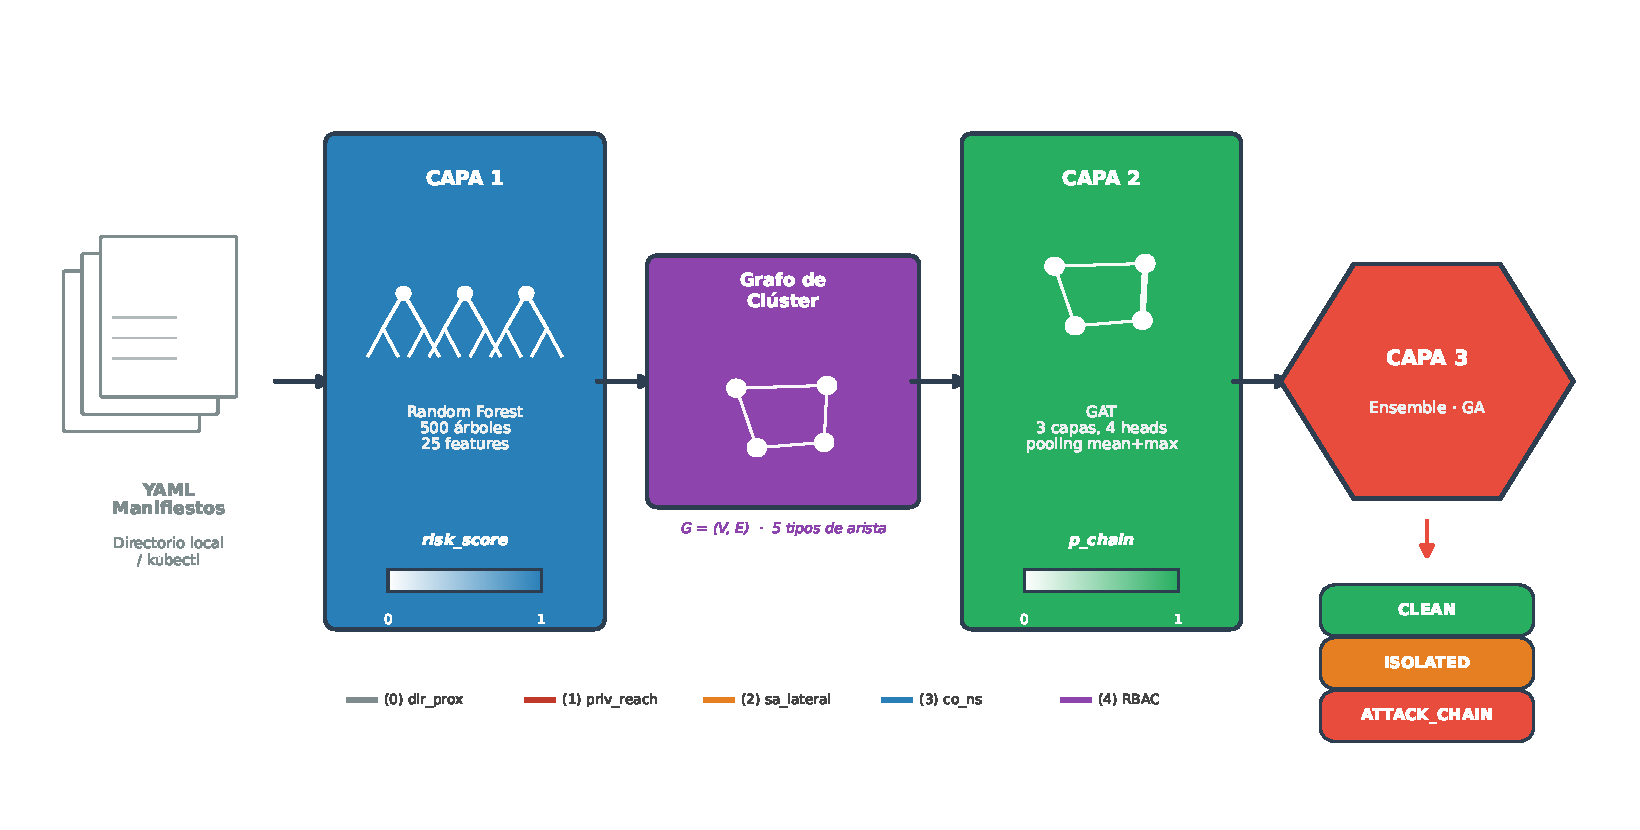
\includegraphics[width=\textwidth]{fig_arquitectura}

  \fuentepropia
\end{figure}

La Figura~\ref{fig:arquitectura} muestra el proceso de tres capas, desde los
manifiestos \acs{YAML} de entrada hasta la clasificación de riesgo del clúster. El
vector de nodo del grafo de entrada de la Capa~2 reserva un atributo adicional
(índice~25) para una puntuación de severidad por manifiesto, calculada como suma
ponderada de las banderas binarias mediante \texttt{compute\_risk\_score}. En el
corpus de entrenamiento esa puntuación es una heurística determinista, no la salida
del clasificador Random Forest; la Sección~\ref{sec:construccion_grafo}
detalla su cobertura efectiva.

% -----------------------------------------------------------
\section{Construcción del conjunto de datos}
\label{sec:construccion_dataset}
% -----------------------------------------------------------

La construcción del conjunto de datos parte de la recolección de manifiestos
\acs{YAML} procedentes de fuentes públicas heterogéneas y avanza hasta la
extracción de las características que alimentan la Capa~1. El origen y la
composición de los manifiestos recopilados determinan la cobertura de patrones de
configuración errónea disponible, y el proceso de extracción de características
transforma cada manifiesto en un vector estructurado de dimensión fija. El
conjunto resultante es la base tanto del clasificador de la Capa~1 como del grafo
de clúster construido en la Sección~\ref{sec:construccion_grafo}.

\subsection{Fuentes de datos}
\label{sec:fuentes_datos}

El conjunto de datos tabular final contiene 2.827~filas y 58~columnas, combinando
cinco fuentes (agrupadas en cuatro categorías, dado que \citet{Rahman2022} aportan dos
plataformas distintas con características de distribución diferentes; ver Tabla~\ref{tab:dataset}):

\begin{table}[htbp]
\centering\small
\caption{Composición del conjunto de datos de manifiestos Kubernetes}
\label{tab:dataset}
\begin{tabular}{@{}p{5.4cm}rp{4.9cm}@{}}
\toprule
Fuente & Filas & Rol \\
\midrule
\citet{Rahman2022} — GitHub & 1.510 & Manifiestos reales, etiquetados \\
\citet{Rahman2022} — GitLab & 396 & Ídem, plataforma distinta \\
BishopFox BadPods \citep{BishopFox2021} & 128 & Pods vulnerables intencionales \\
Kubernetes Goat \citep{KubernetesGoat} & 14 & Escenarios de vulnerabilidad \\
Repositorios de seguridad adicionales & 779 & CTF, \textit{fixtures} de herramientas, labs; etiqueta derivada por regla \\
\midrule
\textbf{Total} & \textbf{2.827} & \\
\bottomrule
\end{tabular}
\fuentepropia
\end{table}

La procedencia de la etiqueta binaria no es homogénea entre las fuentes de la
Tabla~\ref{tab:dataset}, y esa heterogeneidad condiciona la interpretación de los
resultados de la Capa~1. Las 1.906~filas de \citet{Rahman2022}
conservan la anotación \textit{INSECURE} del corpus original, ajena al extractor
de características de este trabajo: solo 245 de las 1.510~filas de GitHub y 87 de
las 396 de GitLab coinciden con la disyunción de las columnas de configuración errónea
observadas. Las 779~filas de los repositorios de seguridad adicionales, en
cambio, carecen de anotación en origen y reciben una etiqueta derivada por regla
en la ingesta (\texttt{compute\_label} en
\texttt{ingest\_attack\_repos.py}), definida como la disyunción de las columnas de
configuración errónea; las 779 satisfacen por construcción esa equivalencia exacta. El
corpus final combina, por tanto, verdad de referencia externa y etiquetado por
regla, circunstancia que se retoma al analizar la circularidad entre etiqueta y
características en la Sección~\ref{sec:rf_importance}.

La incorporación de BadPods fue esencial para mitigar la escasez de ejemplos de
configuraciones erróneas críticas en los repositorios reales: antes de añadir esta fuente,
\texttt{TRUE\_HOST\_PID} aparecía en solo el 0,3\,\% de las filas; tras la incorporación,
la cobertura ascendió al 3,78\,\%. En cuanto a los conjuntos de datos de referencia
existentes para intrusión en red, como UNSW-NB15 \citep{Moustafa2015}, se estudió su
metodología de construcción como guía para el diseño del proceso de etiquetado y la
estrategia de balanceo de clases, dado que sus particiones curadas de entrenamiento y
evaluación presentan un desequilibrio de clases del mismo orden de magnitud que el de
este trabajo (56,3\,\% seguros frente a 43,7\,\% mal configurados). El conjunto GenKubeSec
\citep{Malul2024}, publicado en 2024, no estaba disponible durante el desarrollo de
este trabajo; en su lugar se empleó Checkov \citep{Checkov2021} directamente
sobre los ficheros \acs{YAML} descargados como fuente de validación multiherramienta
equivalente.

\subsection{Características extraídas}

El extractor de características aplica 28 reglas de análisis estático a cada manifiesto
\acs{YAML}, organizadas en tres grupos:

\begin{itemize}
\raggedright
  \item \textbf{18 banderas Rahman} (subconjunto del trabajo original): \texttt{TRUE\_HOST\_PID},
    \texttt{CAP\_SYS\_ADMIN}, \texttt{SEC\_CONT\_OVER\_PRIVIL}, \texttt{INSECURE\_HTTP},
    etc.
  \item \textbf{3 características derivadas}: \texttt{cap\_misuse} (OR de las dos banderas de
    capacidades de sistema), \texttt{all\_secrets} (OR de los indicadores de exposición
    de secretos), \texttt{total\_misconfigs} (suma de todas las banderas activas).
  \item \textbf{7 características extendidas}: \texttt{NO\_RUN\_AS\_NON\_ROOT},
    \texttt{IMAGE\_USES\_LATEST}, \texttt{SA\_AUTOMOUNT\_TOKEN}, \texttt{HOSTPATH\_MOUNT},
    etc. Seis de ellas presentan una procedencia mixta de valores; la séptima,
    \texttt{HOSTPATH\_MOUNT}, se extrae siempre del propio manifiesto.
\end{itemize}

La procedencia de los valores de las seis características extendidas con
equivalente en Checkov \citep{Checkov2021} —\texttt{NO\_RUN\_AS\_NON\_ROOT},
\texttt{NO\_READ\_ONLY\_ROOT\_FS}, \texttt{IMAGE\_USES\_LATEST},
\texttt{SA\_AUTOMOUNT\_TOKEN}, \texttt{USES\_DEFAULT\_SA} y
\texttt{UNTRUSTED\_REGISTRY}— se reparte en tres vías sobre las 2.827~filas del
corpus: 921~filas (32,6\,\%) reciben el valor extraído directamente por el
analizador \acs{YAML}, 1.175~filas (41,6\,\%) se rellenan con la salida de
Checkov a través de la tabla \texttt{CHECKOV\_FILL}, y las 731~restantes
(25,9\,\%) se imputan mediante la mediana de columna. Ese relleno mediante
\texttt{CHECKOV\_FILL} opera exclusivamente en la carga de la Capa~1. El constructor
del grafo lee las columnas de \texttt{FEATURE\_COLS} directamente del conjunto
tabular e imputa como 0 toda celda vacía, sin consultar las columnas
\texttt{checkov\_*}, por lo que las seis características valen 0 en el vector de
nodo de las 1.906~filas procedentes de Rahman et~al. La cobertura de
Checkov tampoco es un mecanismo general aplicable a toda fila con
\acs{YAML} disponible, sino específico de la fuente: Checkov se ejecutó únicamente sobre el subconjunto de
GitHub —1.175 de sus 1.510~filas— y no produjo salida alguna para los
repositorios de seguridad adicionales, GitLab, BadPods ni Kubernetes Goat, cuyas
filas se resuelven por el analizador \acs{YAML} o por mediana. La séptima
característica extendida queda al margen de este esquema, ya que
\texttt{HOSTPATH\_MOUNT} se deriva por completo del análisis estático del
manifiesto y está poblada para las 2.827~filas.

La Capa~2 (\ac{GNN}) consume únicamente las 18~banderas Rahman y las 7~características extendidas
(25 en total, \texttt{FEATURE\_COLS} en \texttt{yaml\_parser.py}) como vector de nodo,
excluyendo las 3~características derivadas —agregados calculados a partir de las otras 25 que
no aportan información estructural adicional al grafo—; ver
Sección~\ref{sec:features_table}. De estas 25, tres presentan varianza casi nula pero
se mantienen en el entrenamiento, con importancia residual o nula
(Sección~\ref{sec:rf_importance}): \texttt{SECCOMP\_UNCONFINED} (15/2.827 activa),
\texttt{VALID\_TAINT\_SECRET} (0/2.827 activa) y \texttt{NO\_NETWORK\_POLICY}
(2.818/2.827 activa, sin poder discriminativo). Las importancias de característica
registradas por el modelo Random Forest confirman ese aporte marginal:
\(1{,}6\times10^{-5}\) para \texttt{SECCOMP\_UNCONFINED}, \(0{,}0\) para
\texttt{VALID\_TAINT\_SECRET} y \(2{,}4\times10^{-5}\) para
\texttt{NO\_NETWORK\_POLICY}. Se conservan para preservar la estabilidad del
contrato de características (\texttt{FEATURE\_COLS}) y la correspondencia exacta
con el conjunto de banderas de \citet{Rahman2022}; no se ha realizado
un estudio de ablación que cuantifique el efecto de su eliminación.

% -----------------------------------------------------------
\section{Construcción del grafo de clúster}
\label{sec:construccion_grafo}
% -----------------------------------------------------------

Cada directorio de manifiestos se representa, mediante NetworkX
\citep{Hagberg2008}, como un grafo dirigido
\(G=(V, E)\) donde \(|V|\) es el número de manifiestos del clúster y
\(E\) contiene aristas de cinco tipos semánticamente distintos
(Tabla~\ref{tab:edge_types}). La Figura~\ref{fig:grafo_cluster} ilustra un ejemplo
con cuatro nodos que incluye los tres tipos de nodo posibles: escape, movimiento
lateral y limpio. Un \textit{namespace} o espacio de nombres es la partición
lógica con la que Kubernetes agrupa y aísla recursos dentro de un mismo clúster,
y delimita el alcance de tres de los cinco tipos de arista. Las reglas de
asignación de cada tipo de nodo y de arista se detallan en las dos subsecciones
siguientes.

\begin{table}[htbp]
\centering\small
\caption{Tipos de aristas en el grafo de clúster}
\label{tab:edge_types}
\begin{tabular}{@{}p{3cm}cp{3.6cm}p{3.8cm}@{}}
\toprule
Tipo & Código & Dirección & Criterio \\
\midrule
Proximidad de directorio & 0 & Bidireccional & Mismos dos componentes finales de ruta \acs{YAML} \\
Alcance de privilegio & 1 & Dirigida (escape\(\to\)mismo \textit{namespace}) & Bandera de escape activa \\
Movimiento lateral \acs{SA} & 2 & Dirigida (lateral\(\to\)mismo \textit{namespace}) & Bandera de movimiento lateral \\
Co-espacio de nombres (\texttt{SEMANTIC\_NS}) & 3 & Bidireccional & Mismo \textit{namespace} K8s \\
Escalada \ac{RBAC} & 4 & Dirigida (elevado\(\to\)mismo \textit{namespace}) & \ac{SA} vinculado a rol privilegiado \\
\bottomrule
\end{tabular}
\fuentepropia
\end{table}

Cada nodo \(v_i\) lleva un vector de características \(\mathbf{x}_i \in \mathbb{R}^{26}\):
los índices 0–24 corresponden a las 25 características binarias de la Capa~1 y el
índice~25 contiene una puntuación de severidad por manifiesto. Esa puntuación
procede de \texttt{compute\_risk\_score}, una suma ponderada de las mismas banderas
binarias normalizada a [0,1], y no de una predicción del clasificador
Random Forest. Está poblada únicamente para los 82~clústeres procedentes
del corpus de Rahman et~al.; en los 517~restantes la columna llega vacía al
constructor del grafo y se imputa como 0, de modo que el índice~25 no aporta señal
en el 86\,\% de los grafos.

\begin{figure}[htbp]
  \centering
  \caption{Ejemplo de grafo de clúster Kubernetes con cuatro nodos}
  \label{fig:grafo_cluster}
  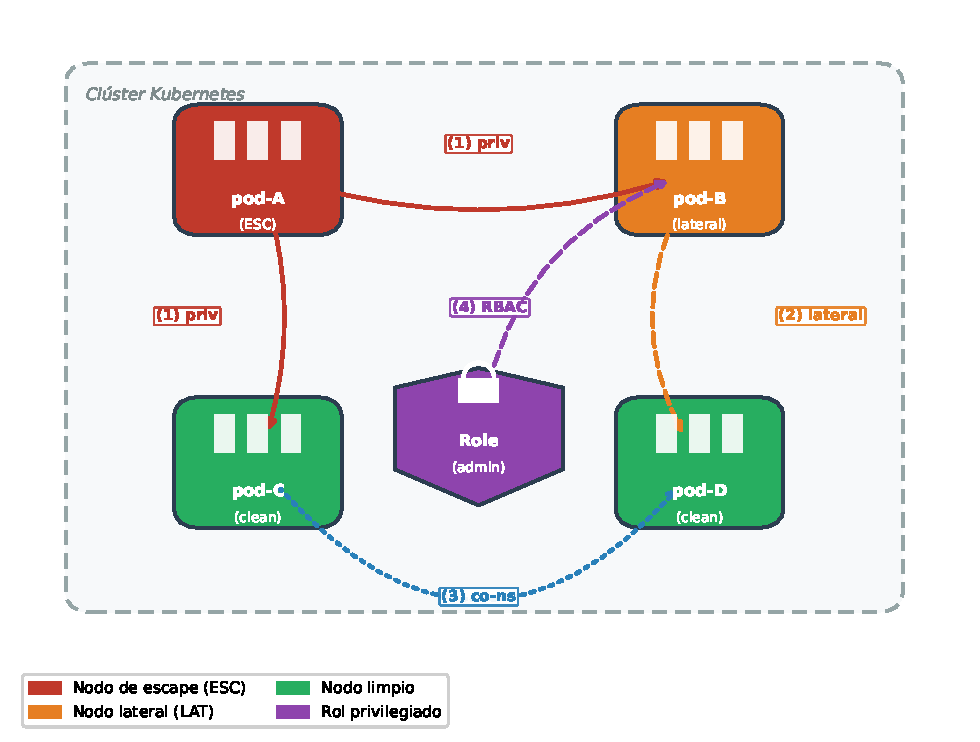
\includegraphics[width=0.72\textwidth]{fig_grafo_cluster}

  \fuentepropia
\end{figure}

La Figura~\ref{fig:grafo_cluster} muestra los tres tipos de nodo (escape, movimiento
lateral y limpio) y las aristas dirigidas que cada uno origina. El nodo rojo (pod-A) tiene
banderas de escape activas y emite aristas de tipo~1 (\textit{privilege\_reach}) hacia
todos los demás nodos de su mismo \textit{namespace}. El nodo naranja (pod-B) tiene banderas de
movimiento lateral y emite aristas de tipo~2 (\textit{sa\_lateral}). La arista de
tipo~4 (\ac{RBAC}) representa la vinculación de un ServiceAccount a un rol
privilegiado.

El conjunto de datos de grafos final comprende 599~grafos originales (25~clean, 537~isolated,
37~attack\_chain) y 1.154~grafos totales tras la aumentación de datos, cuyas variantes
se destinan exclusivamente al conjunto de entrenamiento. De los 555~grafos aumentados
que componen ese \textit{pool}, solo 390 entran efectivamente en el entrenamiento: los
165~restantes derivan de clústeres asignados a validación o test y quedan excluidos por
la regla de asignación consciente de grupos descrita en la
Sección~\ref{sec:aumentacion}. Esta cifra incorpora el corpus
completo de \citet{Rahman2022}, cuyos \textit{namespaces} cruzados
se resolvieron mediante descarga autenticada desde GitHub, lo que amplió
sustancialmente el número de clústeres \textit{isolated} respecto a las fases
experimentales preliminares descritas en la Sección~\ref{sec:layer2} del
Capítulo~\ref{cap:evaluacion}.

\subsection{Detección de escape y movimiento lateral}

{\raggedright
La clasificación de nodos utiliza dos conjuntos de banderas definidos en el código
como constantes inmutables (\texttt{frozenset}). Un nodo se clasifica como de
\textbf{escape} si tiene activa al menos una de las siguientes 8~banderas:
\texttt{TRUE\_HOST\_PID}, \texttt{TRUE\_HOST\_IPC}, \texttt{TRUE\_HOST\_NET},
\texttt{DOCKERSOCK\_PATH}, \texttt{CAP\_SYS\_ADMIN}, \texttt{CAP\_SYS\_MODULE},
\texttt{SEC\_CONT\_OVER\_PRIVIL} o \texttt{HOSTPATH\_MOUNT}. Este último vector fue
incorporado durante el desarrollo al detectar que \textit{badpods\_hostpath} —que monta
el sistema de ficheros del anfitrión— era incorrectamente etiquetado como
\textit{isolated} al no tener ninguna otra bandera de escape activa. Con la corrección,
el número de clústeres de cadena de ataque del corpus preliminar ascendió de 13
a~15; la trayectoria completa del tamaño del corpus y del número de cadenas a lo
largo de las fases experimentales se recoge en la
Tabla~\ref{tab:gnn_evolution}.\par}

Un nodo se clasifica como de \textbf{movimiento lateral} si tiene activa al menos una
de las siguientes 4~banderas: \texttt{SA\_AUTOMOUNT\_TOKEN} (\textit{token} de cuenta de servicio
automontado), \texttt{USES\_DEFAULT\_SA} (usa la cuenta de servicio por defecto del
\textit{namespace}), \texttt{WITHIN\_MANIFEST\_SECRET} (secreto referenciado en el
manifiesto) o \texttt{ALLOW\_PRIVI} (contenedor con capacidad de escalada). Las aristas
de movimiento lateral (tipo~2) se construyen de forma análoga a las de escape: se emite
una arista dirigida desde cada nodo lateral hacia los demás nodos de su mismo
\textit{namespace}.

La convivencia de los cinco tipos sobre un mismo par de nodos se resuelve por orden de
inserción y no por una jerarquía explícita de prioridades. Las aristas se añaden en la
secuencia proximidad de directorio (tipo~0), alcance de privilegio (tipo~1), movimiento
lateral (tipo~2), coespacio de nombres (tipo~3) y escalada \ac{RBAC} (tipo~4). Las de
alcance de privilegio son las únicas que sobrescriben incondicionalmente cualquier
etiqueta previa, de modo que un nodo con capacidad de escape nunca queda degradado a
mero vecino; los cuatro tipos restantes se emiten bajo la guarda \texttt{not
G.has\_edge}, por lo que una arista de proximidad de directorio ya presente impide que
el par se reetiquete como movimiento lateral, y las aristas \ac{RBAC}, al añadirse en
último lugar, nunca desplazan a las de movimiento lateral.

\subsection{Detección de privilegio \acs{RBAC}}

La construcción de aristas \ac{RBAC} (tipo~4) requiere dos pasadas sobre el conjunto de
manifiestos. La primera pasada identifica los roles privilegiados: aquellos cuyo nombre
está en el conjunto \{cluster-admin, admin, edit\} o cuyas reglas contienen verbos de
escalada \{*, escalate, bind, impersonate\}. La segunda pasada recorre los objetos
RoleBinding y ClusterRoleBinding: solo cuando el campo
\textit{roleRef} referencia un rol privilegiado identificado en la primera pasada se
emite una arista \ac{RBAC} desde el pod que usa esa cuenta de servicio hacia los demás
nodos de su mismo \textit{namespace}, coherentemente con el ámbito de los objetos
RoleBinding de los que se derivan las cuentas elevadas.

% -----------------------------------------------------------
\section{Capa 1: Random Forest}
\label{sec:capa1_diseno}
% -----------------------------------------------------------

La Capa~1 clasifica cada manifiesto de forma individual a partir de las
características descritas en la Sección~\ref{sec:construccion_dataset}. Se entrenan dos modelos
independientes sobre el mismo conjunto de características: un clasificador
binario que distingue manifiestos seguros de mal configurados, y un modelo de
severidad que estima el grado de gravedad de la configuración incorrecta
detectada. Ambos comparten el conjunto de 28~características y los mismos
hiperparámetros de bosque, y difieren únicamente en la variable objetivo.

\subsection{Modelo binario}

Se entrena un \texttt{RandomForestClassifier} \citep{Breiman2001} de scikit-learn
\citep{Pedregosa2011} con los hiperparámetros siguientes:

\begin{itemize}
  \item \texttt{n\_estimators = 500}
  \item \texttt{max\_features = sqrt} (clasificación estándar)
  \item \texttt{min\_samples\_leaf = 2} (evita hojas de muestra única)
  \item \texttt{class\_weight = balanced} (compensa ratio 1,29:1)
  \item \texttt{random\_state = 42}
\end{itemize}

El modelo se entrena sobre 2.261~muestras (80\,\% del total) y se evalúa en 566
muestras de test no vistas durante el entrenamiento. La probabilidad predicha para la
clase misconfigured (clase~1) se usa como \textit{risk\_score} del nodo en el grafo.

\subsection{Modelo de severidad}

Además del modelo binario, se entrena un clasificador de severidad de tres clases
(\textit{clean}, \textit{low-medium}, \textit{high-critical}) para ofrecer información
más granular al operador de seguridad. Este modelo no interviene en el cálculo del
grafo; se incluye como salida adicional de la Capa~1.

% -----------------------------------------------------------
\section{Capa 2: Graph Attention Network}
\label{sec:capa2_diseno}
% -----------------------------------------------------------

La Capa~2 opera sobre el grafo de clúster construido en la
Sección~\ref{sec:construccion_grafo} y clasifica el clúster completo según el
riesgo de cadena de ataque que presenta. Su diseño se apoya en tres decisiones
acopladas: una arquitectura \acs{GAT} con \textit{embedding} de tipo de arista, un
procedimiento de entrenamiento con validación cruzada estratificada de
5~pliegues, y una estrategia de aumentación de datos que mitiga la escasez de
clústeres con cadena de ataque confirmada.

\subsection{Arquitectura}

El modelo \ac{GAT} \citep{Velickovic2018} implementado tiene la siguiente estructura,
con las dimensiones exactas verificadas en \texttt{gat\_encoder.py}:

\begin{enumerate}
\raggedright
  \item \textbf{\textit{Embedding} de tipo de arista}: \texttt{Embedding(5, 8)}.
        Los cinco tipos de arista (proximidad de directorio, alcance de
        privilegio, lateral por ServiceAccount, espacio de nombres y
        \ac{RBAC}) son categóricos: codificarlos como un escalar continuo
        implicaría un orden espurio (el tipo~4 «valdría» cuatro veces el
        tipo~1). Cada tipo se proyecta a un vector aprendido de 8~dims que
        \texttt{GATConv} consume como atributo de arista
        (\textit{edge\_dim=8}).
  \item \textbf{Proyección inicial}: \texttt{Linear(26, 256)} \(+\) \texttt{LayerNorm(256)}
        \(+\) \ac{ReLU} \(+\) \texttt{Dropout(0.3)}.
        Proyecta el vector de nodo de 26~dims a 256~dims
        (\(64 \times 4\,\text{cabezas}\)).
  \item \textbf{Capas \ac{GAT}~0 y~1} (\textit{concat=True}):
        \texttt{GATConv(256, 64, heads=4)} con \textit{edge\_dim=8};
        salida 256~dims \((64 \times 4)\); seguidas de \texttt{LayerNorm}, \ac{ELU},
        conexión residual y \texttt{Dropout(0.3)}.
  \item \textbf{Capa \ac{GAT}~2} (\textit{concat=False, heads=1}):
        \texttt{GATConv(256, 64, heads=1)}; salida 64~dims
        (una sola cabeza de atención que produce directamente
        el \textit{embedding} final del nodo, sin concatenación);
        seguida de \texttt{LayerNorm}, \acs{ELU} y \texttt{Dropout(0.3)}
        (sin conexión residual: las dimensiones de entrada y salida difieren,
        256 frente a 64).
  \item \textbf{Global \textit{pooling}}: \texttt{global\_mean\_pool} y \texttt{global\_max\_pool}
        sobre los 64-dim \textit{embeddings} de todos los nodos; concatenación
        \(\to\) 128~dims (\(64 + 64\)).
  \item \textbf{Clasificador \ac{MLP}}: \texttt{Linear(128, 64)} \(+\) \acs{ReLU} \(+\)
        \texttt{Dropout(0.3)} \(+\) \texttt{Linear(64, 3)}.
\end{enumerate}

La elección de \ac{GAT} sobre \ac{GCN} responde a que el mecanismo de atención permite al modelo
aprender qué aristas son más informativas para la señal de ataque: una arista de
\textit{privilege\_reach} debe recibir mayor peso que una arista de proximidad de
directorio. El \textit{pooling} combinado de media y máximo captura dos señales
complementarias: la media refleja la postura de seguridad promedio del clúster,
mientras que el máximo identifica el nodo más peligroso, ambas necesarias para detectar
cadenas de ataque que pueden estar concentradas en un único nodo crítico.

\subsection{Entrenamiento}

El modelo se entrena con PyTorch Geometric \citep{Fey2019}, construido
sobre PyTorch \citep{Paszke2019}, bajo los siguientes hiperparámetros: optimizador AdamW con tasa de aprendizaje
\(5\times10^{-4}\) y \textit{weight\_decay}\,=\,\(10^{-4}\);
\textit{scheduler} CosineAnnealingLR con T\_max\,=\,300 y
\(\eta_{\min}\,=\,10^{-5}\); función de pérdida CrossEntropyLoss con pesos
de clase calculados por frecuencia inversa;
\textit{gradient clipping} con norma máxima 2,0; \textit{early stopping} con
paciencia de 50 épocas; tamaño de lote 8; semilla global 42 (idéntica para el
entrenamiento y para la generación de particiones); y validación cruzada
estratificada de 5~pliegues. El \textit{checkpoint} de cada pliegue se selecciona
por la mejor Precisión@5 de validación, con la F1 macro como criterio de
desempate (\texttt{--select-by p5}), alineando la selección de modelos con la
métrica primaria del sistema en lugar de con la métrica de clasificación.

El guion de entrenamiento (\texttt{train\_gnn.py}) expone tres opciones que
seleccionan variantes de esa configuración y que hacen reproducibles los estudios
de ablación recogidos en el Capítulo~\ref{cap:evaluacion}. La opción
\texttt{-{}-conv} escoge el operador de convolución sobre el grafo entre
\texttt{gat}, la \ac{GAT} con \textit{embedding} de tipo de arista descrita en la
arquitectura y empleado en la configuración desplegada, y \texttt{gcn}, una
\ac{GCN} de referencia que ignora los tipos de arista y pondera todos los vecinos
por igual. La opción \texttt{-{}-focal-loss}, acompañada del parámetro de enfoque
\texttt{-{}-focal-gamma} (valor 2 por defecto), sustituye la entropía cruzada
ponderada por la \textit{focal loss} \citep{Lin2017}, que reduce el peso de los
ejemplos ya bien clasificados para concentrar el gradiente en los difíciles. La
opción \texttt{-{}-select-by} fija el criterio de selección del \textit{checkpoint}
de cada pliegue entre \texttt{f1} (F1 macro de validación) y \texttt{p5}
(Precisión@5 de validación), con la métrica restante como criterio de desempate.
La configuración desplegada corresponde a \texttt{-{}-conv gat}, sin
\texttt{-{}-focal-loss} y con \texttt{-{}-select-by p5}; las alternativas se
cuantifican en las Secciones~\ref{sec:ablacion_perdida}
y~\ref{sec:ablacion_arquitectura}.

Los pesos de clase se calculan en cada pliegue de entrenamiento mediante la
siguiente fórmula implementada en \texttt{train\_gnn.py}:

\begin{equation}
  w_i = \frac{1/n_i}{\displaystyle\sum_{j=0}^{K-1} 1/n_j} \cdot K
  \label{eq:class_weights}
\end{equation}
\addequationtoindex{Cálculo de pesos de clase para el entrenamiento de la GAT}

donde \(n_i\) es el número de grafos de entrenamiento de la clase \(i\) y \(K=3\)
es el número de clases. Esta fórmula normaliza los pesos para que su media sea~1,0,
proporcionalmente equivalente al comportamiento de \texttt{class\_weight=balanced} de
scikit-learn (misma ponderación relativa entre clases). Cabe destacar que los pesos se calculan
\textbf{después} de la aumentación de datos: como la aumentación genera 15~variantes
por grafo de cadena de ataque, la clase \textit{attack\_chain} pasa de ser la
minoría a ser la mayoría en el conjunto de entrenamiento. Los tres recuentos varían de
un pliegue a otro, ya que las variantes de los clústeres reservados para validación se
excluyen en cada iteración: entre 360 y 405~grafos de \textit{attack\_chain} aumentados
frente a 17--18 \textit{clean} y 361--371 \textit{isolated}. La
Ecuación~\ref{eq:class_weights} se autoadapta a esta nueva distribución
asignando mayor peso a \textit{clean} e \textit{isolated}, y menor peso a
\textit{attack\_chain}, compensando el efecto de la sobrerrepresentación creada por
la aumentación.

\subsection{Aumentación de datos}
\label{sec:aumentacion}

Para mitigar la escasez de ejemplos de cadena de ataque (37 de 599 grafos
originales), se aplican tres estrategias de aumentación exclusivamente sobre los
grafos de entrenamiento:

\begin{itemize}
  \item \textbf{\textit{Edge dropout}.} Eliminación aleatoria de entre el 10\,\%
    y el 35\,\% de aristas de los tipos~0 y~3, los menos críticos para la señal de
    ataque, con tasa muestreada uniformemente por variante.

  \item \textbf{\textit{Feature masking}.} Puesta a cero con probabilidad por
    nodo entre el 10\,\% y el 25\,\%, restringida a seis características ajenas a
    la regla de etiquetado de cadena: nunca alcanza las banderas de escape,
    \texttt{HOSTPATH\_MOUNT} ni el \textit{risk\_score}.

  \item \textbf{\textit{Subgraph sampling}.} Extracción de un subgrafo inducido
    por entre el 40\,\% y el 70\,\% de nodos, aplicada a las últimas cinco de las
    15~variantes y solo a grafos de más de 50~nodos, con \textit{BFS} sembrada en
    el nodo de mayor \textit{risk\_score}. Cada subgrafo se valida contra la regla
    de etiquetado de cadena y, si deja de cumplirla, se descarta en favor de una
    variante sobre el grafo completo, lo que evita introducir ruido de etiqueta.
\end{itemize}

Cada grafo de cadena de ataque origina 15~variantes aumentadas, lo que produce
555~grafos adicionales (37~originales \(\times\) 15~variantes) en el
\textit{pool} de aumentación. De estos, únicamente 390 —los correspondientes a
los 26~grafos de cadena cuya base pertenece a la partición de entrenamiento—
entran efectivamente en el entrenamiento, para un total de 1.154~grafos con
aumentación.

La asignación de variantes a particiones es \textbf{consciente de grupos}
(\textit{group-aware}): una variante aumentada solo puede entrar en una partición
de entrenamiento si su grafo base pertenece a esa misma partición. Las variantes
derivadas de clústeres de validación o de test se excluyen del entrenamiento por
completo, ya que entrenar con casi duplicados de un grafo de evaluación
constituiría fuga de datos.

El particionado es además \textbf{consciente de familias de plantilla}: los
clústeres originales que comparten una misma plantilla base (por ejemplo, las
ocho variantes \texttt{badpods\_*}, que difieren únicamente en qué bandera de
escape activan —salvo \texttt{badpods\_nothing-allowed}, que no activa ninguna—,
o las nueve \texttt{datadog\_*}) son casi duplicados entre sí, no
muestras independientes. Cuando una familia contiene etiquetas mixtas, sus
miembros se asignan como una unidad atómica a una única partición —nunca se
reparten entre entrenamiento, validación y test ni entre pliegues— y la
asignación emplea un reparto voraz ponderado por el número de grafos de cada
etiqueta, de modo que la proporción real de cada clase por partición siga las
fracciones solicitadas. Sin esta regla, un modelo entrenado con cinco hermanos de
una familia resuelve trivialmente al sexto en test, inflando las métricas. La
partición resultante (semilla 42) es de 815~grafos de entrenamiento (con
aumentación), 88 de validación y 86 de test. Adicionalmente, los 86~clústeres de
test se mantienen fuera de los pliegues de validación cruzada: los pliegues
particionan únicamente los 513~grafos originales restantes (32 de cadena), de
modo que ni los modelos de pliegue ni las predicciones \textit{out-of-fold}
empleadas para ajustar los pesos del \textit{ensemble} (Capa~3) observan ningún
clúster de test, directa ni indirectamente.

% -----------------------------------------------------------
\section{Capa 3: \textit{Ensemble} con Algoritmo Genético}
\label{sec:capa3_diseno}
% -----------------------------------------------------------

Los pesos \((w_{\text{rf}}, w_{\text{gnn}}, w_{\text{esc}})\) de la
Ecuación~\ref{eq:ensemble} son optimizados mediante un Algoritmo Genético
\citep{Holland1975} con 60~individuos codificados como pares
\((w_{\text{gnn}}, w_{\text{esc}})\) \(\in [0,1]^2\), con \(w_{\text{rf}}\) derivado
como \(1 - w_{\text{gnn}} - w_{\text{esc}}\) (la representación 2D garantiza que la
suma de los tres pesos sea siempre~1). La función objetivo combina la métrica de
\textit{ranking} Precisión@5 y la tasa de falsos positivos sobre clústeres
limpios \ac{FPR}\_clean, ambas definidas en la Sección~\ref{sec:metricas}, junto
con un término de regularización:

\begin{equation}
  F = 0{,}7 \cdot P@5 + 0{,}3 \cdot (1 - \text{FPR\_clean})
      - \lambda \sum_{i} \max(0,\ w_{\min} - w_i)
  \label{eq:ga_fitness}
\end{equation}
\addequationtoindex{Función objetivo (fitness) del Algoritmo Genético}

El último término es una penalización de suelo con \(w_{\min}\,=\,0{,}1\) y
\(\lambda\,=\,2{,}0\): sin ella, el optimizador es libre de anular cualquiera de
los tres pesos cuando eso puntúa marginalmente mejor sobre la muestra
\textit{out-of-fold}, lo que produce soluciones degeneradas que no generalizan al
conjunto de test. La penalización hace que ignorar una señal por completo esté
estrictamente dominado salvo que la ganancia observada supere \(\lambda\) veces el
déficit.

La selección se realiza mediante torneo de tamaño~3, con elitismo del 10\,\%; el cruce
es aritmético (media de los dos padres) con probabilidad 0,7; la mutación combina
perturbación gaussiana (\(\sigma\,=\,0{,}08\), tasa del 15\,\%) con una mutación de
frontera (tasa del 5\,\%) que salta a los vértices del símplex, seguida de
reproyección al dominio válido (\(w_{\text{rf}} \geq 0\)); la población inicial se
siembra con los vértices y puntos medios del símplex y con muestreo de Dirichlet, y el
criterio de parada es 150~generaciones.
Como \textit{baseline} determinista, antes de la optimización genética se
ejecuta una búsqueda en rejilla 2D con paso \(1/20\) (231~evaluaciones); la
comparación de su óptimo con el resultado del \ac{GA} se discute en la
Sección~\ref{sec:layer3}.

La señal de escape se define como un indicador binario que vale~1,0 si al menos un
nodo del clúster tiene alguna bandera de escape activa, y~0,0 en caso contrario. Esta
formulación evita la dilución que produciría una fracción cuando la mayoría de los
nodos del clúster son limpios.

La asignación de clase final a partir de la puntuación \textit{ensemble\_score}
se realiza mediante los siguientes umbrales fijos, definidos en
\texttt{ga\_ensemble.py}:
\begin{itemize}
  \item \textit{ensemble\_score}\,\(\geq\)\,0,60 \(\ \Rightarrow\) \texttt{ATTACK\_CHAIN}
  \item \textit{ensemble\_score}\,\(\geq\)\,0,30 \(\ \Rightarrow\) \texttt{ISOLATED\_MISCONFIG}
  \item De lo contrario \(\Rightarrow\) \texttt{CLEAN}
\end{itemize}
Estos umbrales son fijos y no se reoptimizan durante el entrenamiento del \ac{GA},
que optimiza únicamente los pesos \(w_i\) de la Ecuación~\ref{eq:ensemble}.
Permiten al operador interpretar directamente la puntuación: cualquier clúster con
\textit{score}\,\(\geq\)\,0,60 requiere revisión inmediata.

\subsection{Restricción de viabilidad estructural}
\label{sec:gate_estructural}

Una cadena de ataque multisalto requiere, por definición, alcanzabilidad entre al
menos dos manifiestos; un grafo de clúster con un único nodo no puede albergarla.
Esta propiedad, verificada sobre el corpus completo (los 592~grafos de cadena
—37 originales y 555 variantes aumentadas— tienen \(\geq\)2 nodos y \(\geq\)1 arista,
mientras que 499 de los 537 grafos
\textit{isolated} son de un solo nodo), se incorpora como restricción de
inferencia en \texttt{ga\_ensemble.py} (\texttt{MIN\_CHAIN\_NODES},
\texttt{is\_chain\_feasible}, \texttt{chain\_rank\_key}): en el
\textit{ranking} por riesgo de cadena, ningún clúster de un solo manifiesto puede
superar a un clúster estructuralmente viable, y el veredicto de un clúster
inviable se limita a \texttt{ISOLATED\_MISCONFIG} aunque su puntuación supere el
umbral de 0,60. La restricción se aplica únicamente en inferencia y evaluación;
el ajuste de los pesos del \ac{GA} se realiza sobre el \textit{ranking} sin
restricción, donde los pesos están mejor determinados (la Sección~\ref{sec:layer3}
cuantifica el efecto de esta regla sobre las métricas de test).

% -----------------------------------------------------------
\section{Implementación de kubescan}
\label{sec:implementacion}
% -----------------------------------------------------------

El sistema se distribuye como un paquete Python instalable mediante
\texttt{pip install -e kubescan/}. La estructura del paquete sigue la convención
\textit{src-layout} de \texttt{setuptools}: el código fuente reside en
\texttt{kubescan/src/kubescan/} y los módulos se organizan en tres submódulos:
\texttt{model/} (clasificadores Random Forest, \ac{GAT} y ensamblador \ac{GA}), \texttt{utils/}
(\textit{parser} \acs{YAML} y constructor de grafos) y \texttt{cli.py} (interfaz de
línea de comandos basada en Click).

El punto de entrada principal expone dos comandos. El primero,
\texttt{kubescan scan <dir>}, analiza un directorio local de manifiestos \acs{YAML} y
emite un informe de riesgo en formato texto o \ac{JSON}. El segundo,
\texttt{kubescan live}, consulta la \ac{API} de Kubernetes mediante
\texttt{kubectl}, vuelca los recursos de \textit{workloads} y \ac{RBAC} en un directorio
temporal y ejecuta el \textit{pipeline} completo sobre ellos. La resolución de los
pesos del modelo sigue la cadena: argumento \texttt{--checkpoints-dir}
\(\to\) variable de entorno \texttt{KUBESCAN\_CHECKPOINTS} \(\to\) enlace simbólico
\texttt{kubescan/checkpoints/trained/} \(\to\) \texttt{CheckpointNotFoundError},
excepción tipada derivada de \texttt{KubescanError} y definida en
\texttt{exceptions.py}.

Ambos comandos comparten el conjunto de opciones recogido en la
Tabla~\ref{tab:cli_options} del Anexo~\ref{ap:guia_uso}, definido con
Click en \texttt{cli.py}. La
opción \texttt{-{}-format} selecciona entre el informe en texto y la salida
\ac{JSON}; \texttt{-{}-show-nodes} añade el desglose por manifiesto al informe en
texto; \texttt{-{}-cluster-name} fija el nombre del clúster que encabeza el
informe, que por defecto es el del directorio analizado; y
\texttt{-{}-checkpoints-dir} altera el primer eslabón de la cadena de resolución de
pesos. Las opciones \texttt{-{}-namespace} y \texttt{-{}-all-namespaces} son
exclusivas de \texttt{kubescan live} y delimitan el ámbito de la consulta al
\ac{API} de Kubernetes. El grupo raíz añade, por su parte,
\texttt{-{}-verbose}, que eleva el nivel del registro de \texttt{WARNING} a
\texttt{DEBUG}, y \texttt{-{}-version}, que emite la versión instalada del paquete.

El informe en texto se estructura en tres bloques. El encabezado identifica el
clúster y la ruta analizada. El cuerpo emite el veredicto
(\texttt{CLEAN}, \texttt{ISOLATED\_MISCONFIG} o \texttt{ATTACK\_CHAIN}), seguido de
las señales que lo sustentan —\textit{ensemble score}, probabilidad de cadena del
\textit{ensemble} de cinco pliegues, probabilidad de clúster limpio, riesgo medio del Random Forest,
fracción de manifiestos con capacidad de escape y con capacidad de movimiento
lateral— y de los tres pesos \(w_{\text{rf}}\), \(w_{\text{gnn}}\) y
\(w_{\text{esc}}\) efectivamente aplicados. El bloque final, condicionado a
\texttt{-{}-show-nodes}, tabula los manifiestos ordenados por
\textit{risk\_score} descendente con su marca de escape (\texttt{ESC}) o
movimiento lateral (\texttt{LAT}) y sus primeras cuatro banderas activas. La
Figura~\ref{fig:cli_pipeline} del Anexo~\ref{ap:guia_uso} traza el recorrido
completo de una invocación de \texttt{kubescan scan} y reproduce una
transcripción íntegra de este informe.

La salida \ac{JSON} expone la misma información en un objeto de un solo nivel
apto para consumo automatizado: los campos \texttt{cluster},
\texttt{cluster\_dir} y \texttt{verdict} identifican el análisis; los campos
\texttt{ensemble\_score}, \texttt{chain\_probability},
\texttt{clean\_probability}, \texttt{mean\_rf\_risk} y \texttt{escape\_fraction}
recogen las señales numéricas redondeadas a seis decimales; los recuentos
\texttt{n\_manifests}, \texttt{n\_escape\_capable} y \texttt{n\_lateral\_capable}
resumen la composición del clúster; el objeto anidado \texttt{weights} contiene
los tres pesos del \textit{ensemble}; y la lista \texttt{manifests}, ordenada por
\textit{risk\_score} descendente, aporta por cada manifiesto su nombre de fichero,
su \textit{risk\_score}, los indicadores booleanos \texttt{escape\_capable} y
\texttt{lateral\_capable}, y la lista completa \texttt{flags} de características
de seguridad activas. Estos dos últimos campos son la evidencia de trazabilidad
que verifica el requisito RNF-1 en la
Sección~\ref{sec:verificacion_requisitos}.

% -----------------------------------------------------------
\section{Tabla de características del sistema}
\label{sec:features_table}
% -----------------------------------------------------------

El catálogo completo de las 28~características, con su grupo de procedencia y su
papel en el grafo —detección de escape (ESC) o de movimiento lateral (LAT)—, se
recoge en las Tablas~\ref{tab:features_a}, \ref{tab:features_a2}
y~\ref{tab:features_b} del Anexo~\ref{ap:repositorio}. De las 28, las 25 que no
son derivadas (18~Rahman + 7~extendidas) forman también el vector de nodo de la
Capa~2.

Las 8~banderas de escape (ESC, \texttt{ESCAPE\_FLAGS} en \texttt{graph\_builder.py}) son
\identcode{TRUE\_HOST\_PID}, \identcode{TRUE\_HOST\_IPC}, \identcode{TRUE\_HOST\_NET},
\identcode{DOCKERSOCK\_PATH}, \identcode{CAP\_SYS\_ADMIN}, \identcode{CAP\_SYS\_MODULE},
\identcode{SEC\_CONT\_OVER\_PRIVIL} y \identcode{HOSTPATH\_MOUNT}. Las 4~banderas de movimiento
lateral (LAT, \texttt{LATERAL\_FLAGS}) son \identcode{SA\_AUTOMOUNT\_TOKEN},
\identcode{USES\_DEFAULT\_SA}, \identcode{WITHIN\_MANIFEST\_SECRET} y \identcode{ALLOW\_PRIVI}.
La procedencia de las 7~características extendidas —mixta en seis de ellas y
siempre del propio manifiesto en \identcode{HOSTPATH\_MOUNT}— se detalla en la
Sección~\ref{sec:construccion_dataset}.

% -----------------------------------------------------------
\section{Calidad de software y proceso de desarrollo}
\label{sec:calidad}
% -----------------------------------------------------------

Cuatro herramientas integradas en un
\textit{pipeline} de pre-commit y \acs{CICD} comprueban de forma automática el
estilo, los tipos, el comportamiento y la complejidad del código, y bloquean la
integración cuando alguna comprobación falla: (1) \texttt{ruff}, linter y
formateador con reglas de estilo y seguridad; (2) \texttt{mypy} en modo estricto
(\texttt{mypy kubescan/src -{}-strict}), para el tipado estático de todo el
paquete; (3) \texttt{pytest}, para las pruebas unitarias y de integración; y
(4) \texttt{radon}, para la complejidad ciclomática. El reparto entre ambas
etapas no es uniforme: los \textit{hooks} de pre-commit ejecutan únicamente
\texttt{ruff}, \texttt{ruff-format} y comprobaciones de higiene del repositorio
(espacios finales, fin de fichero, validez de los \acs{YAML} de configuración y
tamaño máximo de los ficheros añadidos), mientras que \texttt{mypy},
\texttt{pytest} y \texttt{radon} se ejecutan en el flujo de integración continua
de GitHub Actions sobre cada \textit{push} y cada \textit{pull request}.

{\raggedright
La suite comprende siete módulos unitarios —analizador \acs{YAML}, constructor
del grafo, codificador \ac{GAT}, clasificador Random Forest, ensamblador \ac{GA},
utilidades de dispositivo y un módulo de pruebas basadas en propiedades con
Hypothesis— y un módulo de integración de extremo a extremo, cuya
verificación funcional se aporta como evidencia de RF-1 y RF-2 en la
Sección~\ref{sec:verificacion_requisitos}. La integración continua ejecuta la
suite con medición de cobertura (\texttt{-{}-cov}). Tres decisiones de diseño
sostienen la reproducibilidad y la seguridad de la carga: \texttt{set\_global\_seed}
centraliza las semillas de \texttt{random}, NumPy y PyTorch;
\texttt{resolve\_device} fija de forma determinista el \textit{backend} de
cómputo; y la carga del clasificador valida los tipos declarados por el fichero
\texttt{skops} contra una lista blanca restringida a scikit-learn y
NumPy, de modo que un \textit{checkpoint} manipulado no pueda introducir
tipos arbitrarios. En el lado de investigación, cada \acs{JSON} de resultados
incorpora un bloque de procedencia con el \textit{commit}, las semillas y las
versiones de los paquetes que lo produjeron.\par}

\startchapter% ============================================================
\chapter{Evaluación}
\label{cap:evaluacion}
% ============================================================

Este capítulo evalúa el sistema kubescan completo. Se parte de una
línea de base tomada del estado del arte, frente a la cual se contrastan los
resultados de cada capa; a continuación se presentan dichos resultados en el
mismo orden que las fases de entrenamiento descritas en el
Capítulo~\ref{cap:herramienta}. El desglose por clases del clasificador de grafo
sobre el conjunto de test (Sección~\ref{sec:gnn_por_clase}) caracteriza la
dirección de los errores residuales, y el contraste con una herramienta de
análisis estático externa (Sección~\ref{sec:validacion_externa}) delimita hasta
qué punto el corpus admite verificación independiente. Sobre esa base se
sintetiza una métrica de proceso completo que resume el comportamiento extremo a
extremo del sistema y se verifica el cumplimiento de los requisitos funcionales y
no funcionales definidos en el Capítulo~\ref{cap:requisitos}. El capítulo cierra
con la evaluación de usabilidad y aplicabilidad realizada con usuarios expertos.
Las métricas empleadas se justifican en detalle en la
Sección~\ref{sec:metricas}.

% -----------------------------------------------------------
\section{Línea de base del estado del arte}
\label{sec:linea_base}
% -----------------------------------------------------------

Antes de presentar los resultados propios, esta sección fija la línea de base
frente a la que se contrastan: los trabajos revisados en el
Capítulo~\ref{cap:estado} que abordan un problema comparable al de cada capa. La
comparación se organiza por capa, dado que la Capa~1 dispone de referencias
directas en la literatura de clasificación de \textit{IaC}, mientras que la
Capa~2 carece de trabajos previos estrictamente comparables. En ambos casos se
prioriza la comparación con resultados obtenidos sobre conjuntos de datos de
tamaño y naturaleza similares; los resultados propios que superan o contrastan
con esta línea de base se presentan en las secciones siguientes.

\subsection{Capa 1 en contexto}

Rahman et~al.\ \citep{Rahman2022}, cuyos datos forman la base del presente
trabajo, no publican modelos de clasificación supervisada sobre el mismo
conjunto: el objetivo de su trabajo era la construcción del conjunto de datos y el
análisis de la densidad de configuraciones erróneas, no la predicción, por lo que no
ofrece una cifra de referencia directa. Tampoco la literatura de \acs{IDS} sobre
UNSW-NB15 \citep{Moustafa2015} proporciona una: ese trabajo presenta el conjunto
de datos y compara exactitud y tasa de falsas alarmas de otros algoritmos, sin
consignar F1 macro ni resultados de Random Forest
(Sección~\ref{sec:ml_vulnerabilidades}). En consecuencia, el umbral
F1\,>\,0,85 de OE2 es un criterio de diseño propio y no una cota tomada de la
literatura, y la comparación informativa para la Capa~1 no es contra ese umbral
sino contra una línea de base trivial calculada sobre el propio corpus: la mejor
regla de una sola característica alcanza F1 macro\,=\,0,8502, frente al 0,9946
del modelo (Sección~\ref{sec:layer1}). Esa separación es consistente
con la naturaleza del problema: las configuraciones erróneas en manifiestos
\acs{YAML} son mayoritariamente discretas y acumulativas (más banderas activas
implica mayor riesgo), lo que hace que el espacio de características sea
relativamente separable una vez que se dispone de un conjunto de datos
suficientemente representativo.

\subsection{Capa 2 en contexto}

Según la revisión bibliográfica no sistemática realizada en este trabajo
(Capítulo~\ref{cap:estado}), no se ha localizado ningún trabajo previo que
aborde la clasificación supervisada de cadenas de ataque en clústeres
Kubernetes mediante \acs{GNN}, por lo que la Capa~2 no dispone de una
línea de base directamente comparable. Las referencias más cercanas son los
trabajos de \acs{GNN} para \ac{IDS} en red, como E-GraphSAGE
\citep{Lo2022}, que documenta tasas de detección superiores a las de
clasificadores tabulares clásicos sobre las re-publicaciones en formato NetFlow
de los conjuntos de referencia del área; y la literatura que documenta la
escasez de conjuntos de datos de grafos etiquetados en ciberseguridad
\citep{GNNSurvey2024}. Cabe puntualizar que esta última no establece un régimen
de tamaño concreto ni prescribe un protocolo de evaluación, de modo que no puede
invocarse como respaldo de la varianza observada en este trabajo; la validación
cruzada estratificada se adopta aquí como decisión metodológica propia. La
ventaja del componente estructural
se mide sobre el conjunto de test genuinamente no visto: P@5 pasa de 0,40
(solo Random Forest) a 0,80 (configuraciones con \ac{GNN}) y P@1 de 0,00 a 1,00
(Tabla~\ref{tab:ensemble_ablation}; Sección~\ref{sec:layer2} y siguientes),
indicando que la información estructural del grafo es decisiva para identificar
cadenas de ataque reales. La varianza entre pliegues de la fase final
(\(\sigma\)\,=\,0,160 para P@5) no se contrasta aquí con ninguna cota externa,
al no disponerse de una referencia que la establezca para conjuntos de este
tamaño; en este trabajo tiene, no obstante, una causa estructural identificada: el
particionado por familias concentra las cadenas de validación de cada pliegue en
1, 1, 4, 5 y 5~familias independientes respectivamente
(Sección~\ref{sec:layer2}), de modo que la desviación estándar entre pliegues
mide en buena parte la dispersión de dificultad entre familias. El análisis
multi-semilla (Sección~\ref{sec:multisemilla}) matiza esa lectura: cuatro de los
cinco pliegues puntúan de forma idéntica con las tres semillas ensayadas, pero el
único que varía —el pliegue~1, correspondiente a la familia
\texttt{badpods\_*}— es también el que más contribuye a esa desviación. En ese
pliegue concreto, la dificultad de la familia y la sensibilidad a la semilla no
resultan separables con los datos disponibles, de modo que la atribución
estructural de la varianza es parcial y no total.

% -----------------------------------------------------------
\section{Resultados de la Capa 1: Random Forest}
\label{sec:layer1}
% -----------------------------------------------------------

Esta sección presenta los resultados de los dos modelos de la Capa~1 descritos en
el Capítulo~\ref{cap:herramienta}: el clasificador binario y el modelo de severidad. Se
presentan primero las métricas de clasificación binaria y la importancia de las
características, y a continuación los resultados del modelo de severidad. Ambos
modelos comparten el mismo conjunto de 28~características extraídas por
manifiesto, descrito en la Sección~\ref{sec:construccion_dataset}.

\subsection{Clasificación binaria}

La Tabla~\ref{tab:rf_results} resume los resultados del modelo binario mediante
cuatro métricas: F1 macro (media no ponderada de F1 entre las clases seguro y
misconfigured, que da igual peso a ambas independientemente de su frecuencia en el
conjunto de datos), exactitud (\textit{accuracy}, porcentaje simple de aciertos), \ac{AUC}-\ac{ROC}
(capacidad del modelo para separar las dos clases a cualquier umbral de decisión) y
\textit{out-of-bag score} (estimación interna de generalización que
Random Forest calcula sobre las muestras que cada árbol no vio durante su
entrenamiento, sin necesitar un conjunto de validación aparte). El clasificador
alcanza una F1 macro de 0,9946 en el conjunto de test, superando el objetivo de
diseño (OE2, F1 macro\,>\,0,85) en 14,5 puntos porcentuales.

Conviene situar esa cifra frente a una línea de base trivial, porque el umbral de
OE2 resulta poco exigente sobre este corpus: la mejor regla de una sola
característica (\texttt{NO\_RESO}\,=\,1) alcanza por sí sola F1 macro\,=\,0,8502,
prácticamente el umbral de 0,85. El margen relevante del modelo no es, por tanto,
el que separa 0,9946 de 0,85, sino el que lo separa de esa regla trivial:
14,4~puntos porcentuales sobre la mejor decisión de una única condición. Una
disyunción de todas las banderas binarias, en cambio, se desploma a
F1 macro\,=\,0,3042, al marcar como mal configurado casi cualquier manifiesto.

\begin{table}[htbp]
\centering
\caption{Resultados del Random Forest — clasificación binaria}
\label{tab:rf_results}
\begin{tabular}{@{}lrrr@{}}
\toprule
Métrica & Test & \acs{CV} (5-fold) & Objetivo \\
\midrule
F1 macro & \textbf{0,9946} & 0,9917 \(\pm\) 0,0053 & \(>0{,}85\) \checkmark \\
Exactitud (\textit{accuracy}) & 0,9947 & 0,9919 \(\pm\) 0,0052 & — \\
\ac{AUC}-\ac{ROC} & \textbf{0,9986} & 0,9984 \(\pm\) 0,0011 & — \\
\textit{Out-of-bag score} & 0,9920 & — & — \\
\bottomrule
\end{tabular}
\fuentepropia
\end{table}

La Figura~\ref{fig:rf_confusion} muestra la matriz de confusión sobre el conjunto
de test (566~muestras). El modelo comete solo 3~errores totales: 3~falsos positivos
(manifiestos seguros clasificados como misconfigured) y 0~falsos negativos.
La ausencia de falsos negativos es la propiedad más crítica para seguridad operativa:
significa que ningún manifiesto con configuraciones erróneas reales escapa al filtrado de
la Capa~1, independientemente de cuántas banderas estén activas o de su rareza en el
conjunto de datos. Los 3~falsos positivos corresponden a manifiestos seguros que acumulan varias
features de riesgo de severidad media (por ejemplo, \texttt{NO\_RUN\_AS\_NON\_ROOT}
y \texttt{IMAGE\_USES\_LATEST} simultáneamente), pero que no tienen ninguna
bandera de escape activa; el operador de seguridad puede descartarlos rápidamente
inspeccionando el campo \texttt{flags} de la salida \ac{JSON}.

El \ac{AUC}-\ac{ROC} de 0,9986 (prácticamente~1,00) indica que el modelo puede ordenar las
muestras por probabilidad de configuración errónea de forma casi perfecta a cualquier umbral
de decisión. En la práctica, este valor implica que, si se ordenan los 566~manifiestos
de test de mayor a menor \textit{risk\_score}, los manifiestos misconfigured aparecen
casi todos antes que los seguros. Esta propiedad es la que habilita el uso del
\textit{risk\_score} como característica nodal cuantitativa en el grafo de la Capa~2:
la señal transmitida a la \ac{GNN} no es un bit binario sino una puntuación
continua que ordena los manifiestos por densidad de configuraciones erróneas. No se
aplica ninguna técnica de calibración de probabilidades, por lo que el valor no
debe interpretarse como una probabilidad calibrada en sentido estricto; el
ordenamiento resultante es, en cambio, consistente con la matriz de confusión de
la Figura~\ref{fig:rf_confusion}.

\begin{figure}[htbp]
  \centering
  \caption{Matriz de confusión del Random Forest en el conjunto de test}
  \label{fig:rf_confusion}
  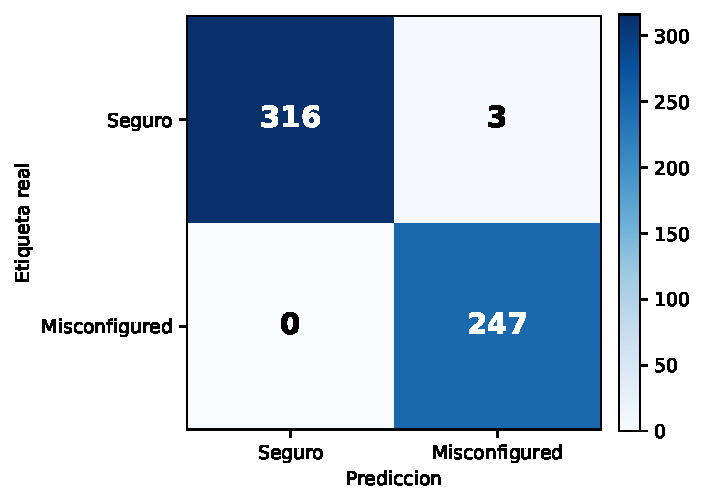
\includegraphics[width=0.52\textwidth]{fig_rf_confusion}

  \fuentepropia
\end{figure}

\subsection{Importancia de características}
\label{sec:rf_importance}

La Figura~\ref{fig:rf_importance} muestra las 10 características más relevantes del
modelo. La característica más discriminativa es \texttt{total\_misconfigs}
(33,05\,\% de importancia), seguida de \texttt{NO\_RESO} (14,79\,\%) e
\texttt{INSECURE\_HTTP} (11,90\,\%). Las banderas de escape críticas (\texttt{TRUE\_HOST\_PID},
\texttt{SEC\_CONT\_OVER\_PRIVIL}) presentan importancias menores (\(<\)1\,\%) por su
rareza en el conjunto de datos, pero son identificadas correctamente cuando están presentes,
como confirma la ausencia de falsos negativos en la clasificación binaria. Las
dos primeras características de la Figura~\ref{fig:rf_importance} (en rojo)
concentran el 48\,\% de la capacidad discriminativa total del modelo. Un estudio
de ablación eliminando \texttt{total\_misconfigs} produce F1 idéntico y la misma
matriz de confusión, lo que confirma que el modelo no depende de esa
característica derivada: su señal es recuperable a partir de las banderas que la
componen.

Esa ablación, sin embargo, no permite concluir que no exista circularidad entre
etiqueta y características. La etiqueta binaria del corpus de Rahman et~al.\ se
define como la presencia de al menos una configuración errónea de un subconjunto
concreto de patrones, y esos patrones son a su vez características de entrada del
modelo: sobre las 1.906~filas de esa fuente, la etiqueta coincide exactamente con
la disyunción de ocho de las características observadas
(\texttt{INSECURE\_HTTP}, \texttt{NO\_SECU\_CONTEXT},
\texttt{WITHIN\_MANIFEST\_SECRET}, \texttt{NO\_RESO}, \texttt{CAP\_SYS\_ADMIN},
\texttt{TRUE\_HOST\_NET}, \texttt{ALLOW\_PRIVI} y \texttt{DOCKERSOCK\_PATH}), sin
un solo falso positivo ni falso negativo. Reentrenar la misma configuración
restringida a esas filas produce, consecuentemente, F1 macro\,=\,1,0000. La Capa~1
aprende por tanto una aproximación robusta de una regla determinista definida
sobre su propio espacio de características —bajo imputación, valores ausentes y
las etiquetas heterogéneas del resto de fuentes—, no una noción de
configuración errónea independiente de dicha regla. Esta limitación, análoga a la que
afecta al etiquetado de grafos, se analiza en la limitación~L5 del
Capítulo~\ref{cap:conclusiones}.

\begin{figure}[htbp]
  \centering
  \caption{Importancia de características del clasificador Random Forest}
  \label{fig:rf_importance}
  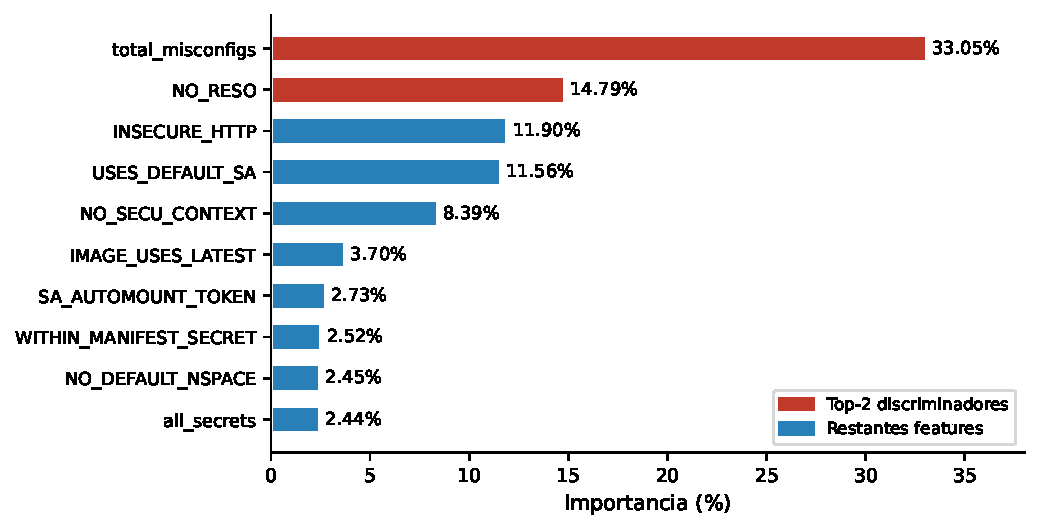
\includegraphics[width=\textwidth]{fig_rf_importance}

  \fuentepropia
\end{figure}

\subsection{Modelo de severidad}

El clasificador de tres clases (\textit{clean}, \textit{low-medium},
\textit{high-critical}) alcanza F1 macro\,=\,0,9838 en test. La Tabla~\ref{tab:severity_f1}
desglosa por clase la precisión (proporción de predicciones de esa clase que son
correctas), el \textit{recall} (proporción de casos reales de esa clase que el
modelo identifica), el F1 (media armónica de ambas) y el soporte (número de
muestras de test en esa clase):

\begin{table}[htbp]
\centering
\caption{F1 por clase — modelo de severidad (3 clases, test)}
\label{tab:severity_f1}
\begin{tabular}{@{}lrrrr@{}}
\toprule
Clase & Precisión & Recall & F1 & Soporte \\
\midrule
\textit{clean}          & 1,0000 & 0,9906 & 0,9953 & 319 \\
\textit{low-medium}     & 0,9615 & 0,9934 & 0,9772 & 151 \\
\textit{high-critical}  & 0,9894 & 0,9688 & 0,9789 & 96 \\
\midrule
Macro media & 0,9836 & 0,9842 & 0,9838 & — \\
\bottomrule
\end{tabular}
\fuentepropia
\end{table}

El F1 más bajo de las tres clases corresponde a \textit{low-medium} (0,9772), por
debajo del de \textit{high-critical} (0,9789). La causa no es una dificultad
intrínseca de la clase intermedia, cuyo \textit{recall} es de 0,9934, sino su
papel de sumidero de los errores del modelo: absorbe los seis manifiestos mal
asignados del conjunto de test —tres procedentes de \textit{clean} y tres de
\textit{high-critical}—, lo que rebaja su precisión a 0,9615. La clase
\textit{high-critical} (96~muestras de test, que representan manifiestos con
banderas de escape activas como \texttt{TRUE\_HOST\_PID} o
\texttt{SEC\_CONT\_OVER\_PRIVIL}) comete 3~errores, los tres clasificados como
\textit{low-medium}; ningún manifiesto crítico es clasificado como
\textit{clean}. Esa ausencia de fugas hacia la clase \textit{clean} es la
propiedad relevante desde el punto de vista de seguridad operativa: en el peor
caso un manifiesto crítico se subestima a \textit{low-medium}, nunca se descarta
como seguro, y la dirección de los errores restantes —tres manifiestos
\textit{clean} sobreclasificados como \textit{low-medium} y un único manifiesto
\textit{low-medium} elevado a \textit{high-critical}— es igualmente conservadora.
El modelo de severidad se utiliza en el informe de salida
de kubescan para proporcionar al operador una descripción cualitativa
del nivel de riesgo de cada manifiesto, complementando el \textit{risk\_score}
numérico del modelo binario.

% -----------------------------------------------------------
\section{Resultados de la Capa 2: \acs{GNN}}
\label{sec:layer2}
% -----------------------------------------------------------

Esta sección presenta los resultados de la Capa~2 en el orden en que fueron
obtenidos durante el desarrollo experimental: la evolución de las métricas a lo
largo de las fases de mejora del modelo, el análisis de Precisión@5, los
resultados por pliegue de la configuración final, la ablación de la función de
pérdida y del criterio de selección, y la robustez frente a la semilla de
entrenamiento. A diferencia de la Capa~1, la Capa~2 requirió varias iteraciones
metodológicas antes de alcanzar una configuración cuyas métricas fueran a la vez
válidas y reproducibles. Cada iteración corrigió una fuente concreta de fuga de
información o una elección de entrenamiento subóptima, y el descenso de las
métricas que acompaña a esas correcciones cuantifica el sesgo optimista que
introducían los protocolos de particionado sucesivamente descartados.

\subsection{Evolución por fase experimental}

La Tabla~\ref{tab:gnn_evolution} muestra la evolución de los resultados de la
\ac{GAT} a lo largo de las seis fases del desarrollo experimental. En las cuatro
primeras, la aumentación de datos y la corrección del vector de escape
\texttt{HOSTPATH\_MOUNT} contribuyeron de forma independiente y complementaria. La quinta fase corrige el protocolo de particionado: las fases~1--4
incluían en el entrenamiento variantes aumentadas derivadas de los
clústeres de validación y test (fuga de datos por casi-duplicados), por lo que sus
métricas están infladas de forma optimista. Esa quinta fase aplica el protocolo
\textit{group-aware} descrito en el Capítulo~\ref{cap:herramienta} (las variantes acompañan a su
clúster base y los clústeres de test quedan fuera de los pliegues) e incorpora el
\textit{embedding} de tipos de arista; sus métricas son metodológicamente válidas
pero corresponden todavía al corpus preliminar de 471~grafos. La sexta y última
fase incorpora el corpus completo de Rahman et~al.\ (599~grafos originales,
37~cadenas; Sección~\ref{sec:construccion_dataset}) y extiende el protocolo de
particionado a las \textbf{familias de plantilla} (Capítulo~\ref{cap:herramienta}):
durante esta fase se detectó que los casi duplicados de una misma plantilla
(ocho \texttt{badpods\_*}, nueve \texttt{datadog\_*}, ocho
\texttt{simulator\_*}, doce \texttt{kubernetes\_goat\_*}) quedaban repartidos
entre particiones, una fuga de información adicional a la de las variantes
aumentadas que inflaba las métricas de las fases 1--5. Con las familias atómicas,
entropía cruzada ponderada como función de pérdida y selección de
\textit{checkpoints} por Precisión@5 (ablación en la
Sección~\ref{sec:ablacion_perdida}), esta fase es la que se presenta como
resultado final del trabajo: sus métricas son las que produce el modelo
efectivamente desplegado y reproducible a partir de los \textit{checkpoints} del
repositorio. Por el cambio de protocolo, sus cifras no son directamente
comparables con las de las fases~1--5 de la Tabla~\ref{tab:gnn_evolution}: miden
generalización entre familias, no interpolación entre casi duplicados.

\begin{table}[htbp]
\centering\small
\caption{Evolución de resultados de la Capa~2 (\acs{GAT}, 5-fold \acs{CV})}
\label{tab:gnn_evolution}
\begin{tabular}{@{}p{4.3cm}rrrrc@{}}
\toprule
Fase & Grafos & Cadenas & F1 macro & P@5 & \shortstack{Cobert.\\techo} \\
\midrule
Línea base & 82 & 13 & 0,829 \(\pm\) 0,098 & 0,400 \(\pm\) 0,179 & 2/5 \\
Tras aumentación & 277 & 13 & 0,915 \(\pm\) 0,059 & 0,520 \(\pm\) 0,098 & 5/5 \\
Tras corrección HOSTPATH & 307 & 15 & 0,915 \(\pm\) 0,050 & 0,600 \(\pm\) 0,000 & 5/5 \\
Conjunto de datos extendido & 471 & 25 & 0,917 \(\pm\) 0,065 & 0,880 \(\pm\) 0,098 & 5/5 \\
Protocolo \textit{group-aware} + \textit{embedding} de aristas
  & 471 & 25 & 0,870 \(\pm\) 0,075 & 0,720 \(\pm\) 0,098 & 3/5 \\
\addlinespace
Corpus completo + familias de plantilla (final)
  & 599 & 37 & \textbf{0,803 \(\pm\) 0,137} & \textbf{0,720 \(\pm\) 0,160} & 1/5 \\
\bottomrule
\end{tabular}
\fuentepropia
\end{table}

En la Tabla~\ref{tab:gnn_evolution}, las fases 1--4 emplean el protocolo de
particionado preliminar (con fuga por variantes aumentadas) y se conservan como
registro histórico; la fase~5 introduce el protocolo \textit{group-aware} sobre el
corpus preliminar; la fase~6 es el resultado final, con protocolo
\textit{group-aware} sobre el corpus completo.
La columna «Cobert.\ techo» indica en cuántos de los 5~pliegues el modelo alcanza
el \emph{techo teórico} de P@5. La métrica se calcula como el número de cadenas
situadas en el top-5 dividido entre \(\min(5,\, n_{\text{pos}})\), siendo
\(n_{\text{pos}}\) el número de cadenas presentes en el pliegue, de modo que el
techo vale 1,0 siempre que el pliegue contenga al menos una cadena y se alcanza
cuando las cinco primeras posiciones del \textit{ranking} están ocupadas por
cadenas —o, si el pliegue contiene menos de cinco, cuando todas ellas figuran en
el top-5. En la fase final, los cinco pliegues de validación contienen 8, 7, 6, 6
y 5~cadenas respectivamente, por lo que el denominador es 5 en todos ellos y el
techo 1,0 exige cinco aciertos en las cinco primeras posiciones; únicamente el
pliegue~0 lo consigue.

Las cuatro primeras fases de la Tabla~\ref{tab:gnn_evolution} corresponden al
protocolo preliminar. El objetivo de diseño de \textit{ranking} es P@5\,>\,0,70 y el umbral
de F1 fijado para la Capa~1, tomado como referencia, 0,85; las desviaciones típicas
representan la desviación estándar entre los 5~pliegues de validación cruzada.

\subsection{Análisis de Precisión@5}

El objetivo de diseño es P@5\,>\,0,70 (OE4). En el resultado final de este trabajo
—particionado consciente de familias sobre el corpus completo de Rahman et~al.
(599~grafos originales, 37~cadenas; fase~6 de la Tabla~\ref{tab:gnn_evolution})—
los pliegues de validación cruzada particionan los 513~grafos originales no
reservados para test (32~cadenas). El modelo obtiene
P@5\,=\,0,720\,\(\pm\)\,0,160, alcanzando el objetivo con la semilla de
entrenamiento desplegada (42); en las tres semillas (7, 42, 123) la media es
de 0,68\,\(\pm\)\,0,03\footnote{Las desviaciones típicas de las métricas del modelo
se expresan como desviación poblacional (\(\text{ddof}=0\)), consistente con la
instrumentación de NumPy empleada en la validación cruzada; la del \ac{SUS}
(Sección~\ref{sec:usabilidad}) sigue la convención muestral (\(n-1\)) habitual en su
literatura.}, con el objetivo dentro de una desviación típica de la
media (Sección~\ref{sec:multisemilla}).

Alcanzar esta cifra exigió diagnosticar una regresión aparente: la primera
configuración entrenada sobre el corpus completo con familias atómicas empleaba
\textit{focal loss} y selección de \textit{checkpoints} por F1 macro, y obtuvo
P@5\,=\,0,480\,\(\pm\)\,0,271, muy por debajo tanto del objetivo como de la
fase~5. La ablación factorial de la Sección~\ref{sec:ablacion_perdida} mostró
que la caída se debía a las elecciones de función de pérdida y de criterio de
selección —no al corpus ni al protocolo de particionado—, y que revertir a
entropía cruzada ponderada y seleccionar por Precisión@5 recupera el objetivo
sobre el mismo particionado honesto. La varianza entre pliegues
(\(\sigma\)\,=\,0,160, frente a 0,098 en la fase~5) refleja en gran medida la
propia atomicidad de las familias: cada pliegue evalúa 1, 1, 4, 5 y
5~familias independientes respectivamente, como se detalla a continuación.

\subsection{Resultados por pliegue (fase final)}

Las medias de validación cruzada de la configuración desplegada ocultan una
dispersión considerable entre pliegues, y su desglose es necesario para atribuir
esa dispersión a una causa concreta. La Tabla~\ref{tab:gnn_folds} recoge la F1
macro y la Precisión@5 obtenidas en cada uno de los cinco pliegues, junto con la
media y la desviación típica poblacional que resumen el conjunto. Los valores
individuales se interpretan a continuación a la luz de la composición de cada
pliegue en términos de familias de plantilla.

\begin{table}[htbp]
\centering
\caption{Resultados por pliegue — Capa~2, fase final}
\label{tab:gnn_folds}
\begin{tabular}{@{}crr@{}}
\toprule
Pliegue & F1 macro & P@5 \\
\midrule
0 & 1,000 & 1,00 \\
1 & 0,580 & 0,60 \\
2 & 0,863 & 0,60 \\
3 & 0,801 & 0,60 \\
4 & 0,770 & 0,80 \\
\midrule
\textbf{Media} & \textbf{0,803} & \textbf{0,720} \\
\textbf{\(\pm\) Desv.} & \textbf{0,137} & \textbf{0,160} \\
\bottomrule
\end{tabular}
\fuentepropia
\end{table}

La Tabla~\ref{tab:gnn_folds} corresponde al particionado consciente de familias
sobre el corpus completo: los pliegues particionan 513~grafos originales con
32~cadenas, con el conjunto de test excluido.
La dispersión entre pliegues es consecuencia directa del particionado por
familias: al mantener cada familia de plantilla como unidad atómica, las cadenas
de validación de cada pliegue quedan concentradas en pocas familias
independientes. El pliegue~0 valida sobre las nueve variantes \texttt{datadog\_*}
(ocho de ellas cadenas; grafos de 2--3 nodos casi idénticos entre sí) y alcanza
F1\,=\,1,0 y P@5\,=\,1,0; el pliegue~1 valida sobre las ocho variantes
\texttt{badpods\_*} (siete de ellas cadenas) y
es sistemáticamente el más difícil (P@5\,=\,0,60 con la semilla desplegada;
0,2--0,6 según la semilla, Sección~\ref{sec:multisemilla}). Los tres pliegues
restantes reparten las dos familias grandes que quedan junto a repositorios
únicos: el pliegue~2 concentra las ocho variantes \texttt{simulator\_*}, el
pliegue~3 las doce variantes \texttt{kubernetes\_goat\_*} y el pliegue~4 no
contiene ninguna de las cuatro familias de plantilla, sino exclusivamente
repositorios únicos. El número de familias independientes portadoras de cadena
por pliegue es, en consecuencia, de 1, 1, 4, 5 y 5. Cada pliegue mide, por tanto,
la capacidad del modelo de generalizar a un número reducido de familias no vistas
—un tamaño muestral efectivo menor que el número nominal de cadenas—, lo que
explica que la varianza
(\(\sigma\)\,=\,0,160) sea mayor que bajo protocolos con fuga y constituye una
amenaza a la validez de conclusión que se documenta en el
Capítulo~\ref{cap:conclusiones}.

\subsection{Ablación de función de pérdida y criterio de selección}
\label{sec:ablacion_perdida}

La regresión aparente de la primera configuración sobre el corpus completo
(P@5\,=\,0,480) confundía dos cambios simultáneos: la introducción de
\textit{focal loss} \citep{Lin2017} y el nuevo particionado por familias. Para
atribuir el efecto se completó la matriz factorial 2\(\times\)2 —función de
pérdida (entropía cruzada ponderada frente a \textit{focal loss},
\(\gamma\)\,=\,2) por criterio de selección de \textit{checkpoints} (F1 macro
frente a Precisión@5)— con particionado, semilla y arquitectura idénticos
(Tabla~\ref{tab:loss_ablation}).\footnote{Las cuatro configuraciones son reproducibles
mediante \texttt{make reproduce GNN\_FOCAL=\{0,1\} GNN\_SELECT\_BY=\{p5,f1\}}; solo se
conserva el \textit{checkpoint} de la configuración finalmente desplegada.}

\begin{table}[htbp]
\centering
\caption{Ablación de función de pérdida y criterio de selección}
\label{tab:loss_ablation}
\begin{tabular}{@{}llrr@{}}
\toprule
Pérdida & Selección & P@5 (\acs{CV}) & F1 macro (\acs{CV}) \\
\midrule
\textit{Focal} (\(\gamma\)=2) & F1 macro & 0,480 \(\pm\) 0,271 & 0,823 \(\pm\) 0,097 \\
Entropía cruzada pond. & F1 macro & 0,600 \(\pm\) 0,283 & 0,859 \(\pm\) 0,103 \\
\textit{Focal} (\(\gamma\)=2) & P@5 & 0,680 \(\pm\) 0,204 & 0,795 \(\pm\) 0,173 \\
Entropía cruzada pond. & P@5 & \textbf{0,720 \(\pm\) 0,160} & 0,803 \(\pm\) 0,137 \\
\bottomrule
\end{tabular}
\fuentepropia
\end{table}

Las cuatro configuraciones de la Tabla~\ref{tab:loss_ablation} se evaluaron con
5-fold \ac{CV} sobre el corpus completo, particionado por familias y semilla~42.
Los dos efectos principales apuntan en la misma dirección, pero no se comportan
de forma aditiva: sustituir \textit{focal loss} por entropía cruzada ponderada
aporta +0,12~puntos de P@5 con selección por F1 macro y solo +0,04 con selección
por P@5, mientras que seleccionar los \textit{checkpoints} por la métrica
primaria de \textit{ranking} en lugar de por F1 macro aporta +0,20~puntos bajo
\textit{focal loss} y +0,12 bajo entropía cruzada. La suma de ambos efectos
principales sobre la configuración de partida (0,480) predeciría
P@5\,=\,0,80, frente al 0,720 efectivamente observado: existe una interacción
negativa de 0,08~puntos, es decir, la mejora que aporta cada factor se solapa
parcialmente con la del otro en lugar de acumularse. La \textit{focal loss},
diseñada para regímenes con miles de ejemplos por clase \citep{Lin2017}, además
anula por completo la clasificación de la clase \textit{attack\_chain} en el
conjunto de test (F1 de clase 0,0 frente a 0,667 con entropía cruzada). La
configuración desplegada es, en consecuencia, entropía cruzada ponderada con
selección por Precisión@5.

La Tabla~\ref{tab:loss_ablation} recoge la Precisión@5 de validación cruzada
(\(\pm\)\(\sigma\)) de las cuatro configuraciones; solo la desplegada —entropía
cruzada ponderada con selección por Precisión@5— supera el objetivo de diseño.
La distancia respecto de la segunda mejor configuración es, no obstante, estrecha
(0,720\,\(\pm\)\,0,160 frente a 0,680\,\(\pm\)\,0,204): sus bandas de una
desviación típica se solapan casi por completo y, sobre cinco pliegues y con una
métrica cuantizada en múltiplos de 0,2, esa diferencia equivale a un solo acierto
de \textit{ranking} en un único pliegue. Los datos sostienen, por tanto, una
afirmación más débil que la de una dependencia estricta de ambos factores: la
combinación desplegada es la única que sitúa la media de validación cruzada por
encima del objetivo, y la configuración más alejada de él —\textit{focal loss}
con selección por F1 macro, 0,480— sí queda separada por un margen que excede la
dispersión observada.

\subsection{Ablación de arquitectura}
\label{sec:ablacion_arquitectura}

La elección de \ac{GAT} frente a alternativas más simples y la profundidad de
tres capas se fijaron en el diseño de la Capa~2 y admiten contraste empírico
sobre el mismo protocolo. La literatura sobre \acs{GNN} aplicadas a grafos
pequeños heterogéneos documenta de forma consistente que los mecanismos de
atención mejoran la precisión cuando los tipos de arista tienen importancias
desiguales \citep{Velickovic2018}. En el grafo de clúster
Kubernetes, las aristas de \textit{privilege\_reach} (tipo~1) son
cualitativamente más informativas que las de \textit{dir\_proximity} (tipo~0): la
primera conecta directamente nodos de escape con el resto del clúster, mientras que
la segunda simplemente refleja la organización de directorios del repositorio.
\ac{GAT} puede aprender esta distinción durante el entrenamiento, mientras que \ac{GCN} asigna
pesos uniformes a todos los vecinos, diluyendo la señal de escape con ruido de
co-localización.

Esta hipótesis se cuantifica empíricamente mediante un experimento de ablación
controlado sobre el corpus completo, con particionado, semilla, función de
pérdida y criterio de selección idénticos a los de la configuración final
(fase~6 de la Tabla~\ref{tab:gnn_evolution}), de modo que las tres filas son
directamente comparables entre sí y con el resultado final (Tabla~\ref{tab:arch_ablation}):

\begin{table}[htbp]
\centering
\caption{Ablación de arquitectura — Capa~2}
\label{tab:arch_ablation}
\begin{tabular}{@{}lrr@{}}
\toprule
Arquitectura & F1 macro & P@5 \\
\midrule
\ac{GAT} 3 capas + \textit{embedding} de aristas (desplegada)
  & \textbf{0,803 \(\pm\) 0,137} & \textbf{0,720 \(\pm\) 0,160} \\
\ac{GAT} 2 capas + \textit{embedding} de aristas
  & 0,800 \(\pm\) 0,171 & \textbf{0,720 \(\pm\) 0,160} \\
\ac{GCN} 3 capas (sin tipos de arista)
  & 0,711 \(\pm\) 0,143 & 0,680 \(\pm\) 0,160 \\
\bottomrule
\end{tabular}
\fuentepropia
\end{table}

La \ac{GAT} supera a la \ac{GCN} en F1 (+9,2~puntos) y en P@5 (+4~puntos). Esa
ventaja acredita la configuración adoptada en su conjunto, pero no permite
atribuirla al esquema de tipos de arista por separado: la rama \ac{GCN} sustituye
simultáneamente el mecanismo de agregación por atención y descarta el tensor
\texttt{edge\_attr}, de modo que ambos factores varían a la vez. Aislar la
contribución del tipado exigiría una tercera rama —\ac{GAT} sin tipos de arista—
que no forma parte de las configuraciones entrenadas
(Capítulo~\ref{cap:conclusiones}). La comparación entre 2 y 3~capas es
menos concluyente: las medias de validación cruzada casi coinciden
—P@5\,=\,0,720\,\(\pm\)\,0,160 en ambas configuraciones y F1 macro de 0,803
frente a 0,800—, pero esa coincidencia agregada oculta un desacuerdo apreciable
pliegue a pliegue, con diferencias de F1 de \(+\)0,142 en el pliegue~3 y
\(-\)0,191 en el pliegue~4 que se cancelan al promediar y dejan una brecha media
de solo 0,003. Dos modelos que difieren en esa magnitud sobre pliegues concretos
no evidencian robustez de la arquitectura frente a la profundidad, sino que la
profundidad no determina el nivel medio de las métricas sobre este corpus. Se
mantiene la configuración de 3~capas como desplegada por su ventaja marginal en
F1 macro y por coherencia con el resto de resultados presentados. La
ablación de \textit{pooling} (\textit{mean}-only frente a \textit{mean+max}) queda
como trabajo futuro (TF6, Sección~\ref{sec:trabajo_futuro}).

\subsection{Robustez frente a la semilla de entrenamiento}
\label{sec:multisemilla}

Para acotar la dependencia del resultado respecto de la semilla de entrenamiento,
la configuración final se reentrenó con tres semillas (7, 42, 123;
Figura~\ref{fig:multiseed_folds}) manteniendo fijo el particionado (semilla~42):
re-sortear también las particiones confundiría la varianza del modelo con la
asignación de familias a pliegues, que la Sección~\ref{sec:layer2} muestra
dominante. Las métricas de test aplican la restricción de viabilidad estructural
(Sección~\ref{sec:gate_estructural}).

Dos observaciones acotan la lectura del 0,72. Primera: la variación entre
semillas se concentra íntegramente en el pliegue~1 (la familia
\texttt{badpods\_*}: P@5 de 0,2/0,4/0,6 según semilla), mientras que los otros
cuatro pliegues puntúan de forma idéntica con las tres semillas. Esa coincidencia
impide leer el experimento como una demostración de estabilidad global, porque el
único pliegue sensible a la semilla es precisamente el que domina la desviación
típica entre pliegues: en él, la dificultad de la familia y la variabilidad de
entrenamiento quedan confundidas y no pueden separarse con tres semillas. Lo que
el experimento sí establece es que cuatro quintas partes del particionado son
invariantes a la semilla y que la incertidumbre residual de la estimación de
validación cruzada se localiza en una sola familia de plantilla. Segunda: las
métricas de test a nivel de despliegue son estables —P@1\,=\,1,00 y
P@3\,=\,1,00 con las tres semillas, y P@5 entre 0,80 y 1,00—, de modo que la
sensibilidad a la semilla afecta a la estimación de validación cruzada, no al
comportamiento observable del sistema sobre repositorios reales no vistos.

\begin{figure}[htbp]
  \centering
  \caption{Precisión@5 por pliegue con tres semillas de entrenamiento}
  \label{fig:multiseed_folds}
  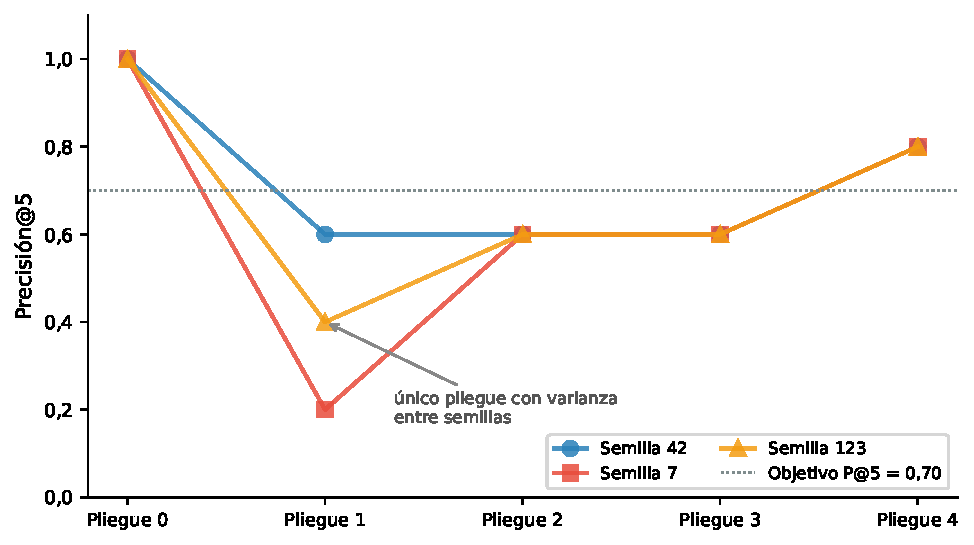
\includegraphics[width=0.85\textwidth]{fig_multiseed_folds}

  \fuentepropia
\end{figure}

% -----------------------------------------------------------
\section{Resultados de la Capa 3: \textit{Ensemble}}
\label{sec:layer3}
% -----------------------------------------------------------

El ajuste de los pesos del \textit{ensemble} atravesó dos correcciones metodológicas
sucesivas, ambas implementadas en \texttt{run\_ga\_ensemble.py}. En una primera
iteración, el \ac{GA} original convergía sistemáticamente a pesos casi uniformes
\((w_{\text{rf}}, w_{\text{gnn}}, w_{\text{esc}}) \approx (0{,}34,\, 0{,}33,\, 0{,}33)\)
sin mejorar sobre su población inicial en 150~generaciones, un patrón que parecía
indicar una meseta plana en la función de \textit{fitness}. Un diagnóstico
descartó esa hipótesis: el cruce por promedio aritmético es contractivo y no
puede alcanzar los vértices del símplex de pesos desde una población inicializada
por muestreo de Dirichlet, y la mutación gaussiana (\(\sigma=0{,}08\)) es
demasiado local para recorrer esa distancia en 150~generaciones. La primera
corrección sembró los vértices y aristas del símplex en la población inicial y
añadió una mutación de salto de frontera de baja probabilidad; con este cambio,
el \ac{GA} pasó a converger de forma determinista, en las 5~semillas
independientes probadas, al mismo punto que una búsqueda en rejilla
determinística (Sección~\ref{sec:capa3_diseno}, 231~evaluaciones): el vértice de
señal de escape pura (\(w_{\text{esc}}=1\), \textit{objective}\,=\,0,86),
confirmando que la función objetivo tenía un óptimo global único y alcanzable, no
una meseta degenerada. Sin embargo, ese óptimo \textit{out-of-fold} no
generalizaba: al puntuar únicamente por la señal binaria de escape, el \textit{ranking} se
colapsaba a un grupo de empates que fallaba estructuralmente ante cualquier
cadena de ataque cuya única señal fuerte no fuera la bandera de escape.

Esta segunda observación motivó la corrección definitiva: regularizar la propia
función objetivo con una penalización de piso,
\(F = \alpha \cdot P@5 + \beta \cdot (1-\text{\ac{FPR}\_clean}) -
\lambda \sum_i \max(0,\, w_{\min} - w_i)\), con \(w_{\min}=0{,}1\) y
\(\lambda=2{,}0\) (opciones \texttt{--min-weight}/\texttt{--reg-lambda}). Esta
penalización hace que el vértice de escape puro deje de ser competitivo frente a
soluciones interiores del símplex. Sobre el conjunto \textit{out-of-fold} de la
configuración final (513~grafos, 32~cadenas), el \ac{GA} regularizado encuentra
su mejor solución ya en la generación inicial y no la mejora durante las
150~generaciones:
\((w_{\text{rf}}, w_{\text{gnn}}, w_{\text{esc}}) = (0{,}517,\, 0{,}115,\, 0{,}368)\),
\textit{objective}\,=\,0,72. La búsqueda en rejilla encuentra un punto muy
distinto (\(w_{\text{rf}}=0{,}80,\, w_{\text{gnn}}=0{,}10,\,
w_{\text{esc}}=0{,}10\)) con idéntica P@5 \textit{out-of-fold}: al ser P@5 una
función escalonada (solo toma valores múltiplos de 0,2), la función objetivo
presenta mesetas extensas en las que los pesos quedan \textbf{indeterminados}.
Esta indeterminación es medible: sobre el conjunto de test, los pesos elegidos
por el \ac{GA} y los pesos uniformes \((1/3)\) producen métricas idénticas
(Tabla~\ref{tab:ensemble_ablation}). Contribuye a ella un desplazamiento de
distribución entre el conjunto de ajuste y el de test: 15 de las 32~cadenas
\textit{out-of-fold} pertenecen a familias de \textit{fixtures} sintéticas
(\texttt{badpods\_*}, \texttt{datadog\_*}) cuyos manifiestos reciben
\textit{risk scores} altos del Random Forest, mientras que las cinco cadenas de test son
repositorios reales cuyo \textit{risk score} medio por clúster es
\(\approx\)0 (la media se diluye entre manifiestos mayoritariamente benignos).
Tres refinamientos del ajuste (un término de desempate por \textit{mean
reciprocal rank}, la agregación del \textit{pool} por familias y el ajuste sobre
el \textit{ranking} con restricción estructural) se implementaron y evaluaron
sin que ninguno mejorara las métricas de test, por lo que los pesos se ajustan
sobre el \textit{ranking} sin restricción y la restricción de viabilidad
estructural (Sección~\ref{sec:gate_estructural}) se aplica en inferencia y
evaluación.

La evaluación final se realiza sobre el conjunto de test (86~grafos: 3~limpios,
78~\textit{isolated} y 5~cadenas de ataque; techo P@5\,=\,1,00). Bajo el
particionado consciente de familias, las cinco cadenas son repositorios reales
únicos —sin hermanos de plantilla en el entrenamiento— excluidos de los pliegues
de validación cruzada, del ajuste de pesos del \ac{GA} y del entrenamiento con
variantes aumentadas: no vistos en ningún momento del desarrollo. Con la
restricción de viabilidad estructural aplicada al \textit{ranking}
(Sección~\ref{sec:gate_estructural}), el \textit{ensemble} alcanza P@1\,=\,1,00,
P@3\,=\,1,00 y P@5\,=\,0,80: las cadenas ocupan las posiciones 1--4 y 6, y solo
\texttt{minik8s-ctf} queda fuera del top-5. Sin la restricción, las métricas
caen a P@1\,=\,0,00, P@3\,=\,0,33 y P@5\,=\,0,60 (Figura~\ref{fig:structural_gate}): la regla es decisiva porque
74 de los 86~grafos de test son de un solo nodo, y dos de ellos, con todas sus
banderas de escape activas, encabezarían el \textit{ranking} pese a no poder
albergar una cadena. Procede delimitar, en consecuencia, cuál es el conjunto sobre
el que se ordena: la restricción deja 12~clústeres candidatos —las 5~cadenas,
4~\textit{isolated} y 3~limpios—, de modo que las métricas de \textit{ranking} no
se calculan sobre los 86~grafos sino sobre esos 12. Un ordenamiento aleatorio de
ese conjunto obtendría un valor esperado de P@5 de \(5/12 \approx 0{,}42\), que
es la línea de base frente a la que debe leerse el 0,80 obtenido.
\ac{FPR}\_clean\,=\,0,00: ningún clúster limpio aparece
entre los de mayor riesgo. La F1~macro por clasificación \textit{argmax} del
\textit{ensemble} de pliegues sobre el conjunto de test es 0,883 (F1 por clase:
\textit{clean} 1,0; \textit{isolated} 0,981; \textit{attack\_chain} 0,667,
con 3 de las 5~cadenas correctamente clasificadas).

\begin{figure}[htbp]
  \centering
  \caption{Efecto de la restricción de viabilidad estructural}
  \label{fig:structural_gate}
  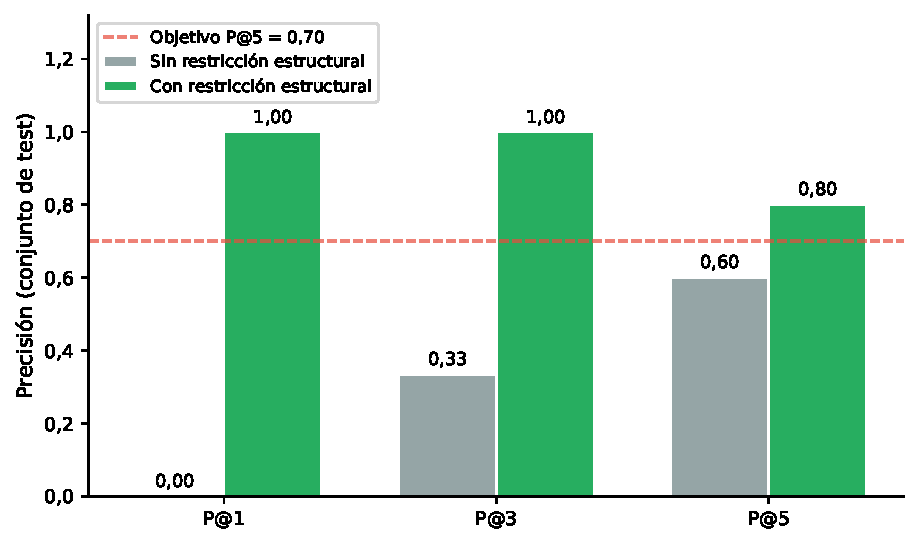
\includegraphics[width=0.82\textwidth]{fig_structural_gate}

  \fuentepropia
\end{figure}

Dado el tamaño del conjunto de test, estas estimaciones llevan asociados
intervalos de confianza amplios (bootstrap de 10\,000 remuestreos, 95\,\%):
P@5 \([0{,}60,\ 1{,}00]\), \ac{FPR}\_clean \([0{,}00,\ 0{,}40]\) y F1~macro
\([0{,}66,\ 1{,}00]\). Los valores puntuales deben interpretarse como
\textit{consistentes con} los objetivos de diseño, no como demostraciones
concluyentes; la ampliación adicional del corpus de test es la vía directa para
estrechar estos intervalos (TF1, Sección~\ref{sec:trabajo_futuro}). La
Tabla~\ref{tab:ensemble_ablation} recoge las tres métricas de \textit{ranking} del
\textit{ensemble} sobre el conjunto de test.

La Tabla~\ref{tab:ensemble_ablation} desglosa la contribución de cada componente
sobre el conjunto de test (86~grafos, 5~cadenas, techo P@5\,=\,1,00), con la
restricción de viabilidad estructural aplicada
en todas las configuraciones. De la ablación se desprenden tres observaciones:

\begin{enumerate}
  \item La configuración con solo Random Forest degrada gravemente el
    \textit{ranking} (P@1\,=\,0,00, P@5\,=\,0,40). El \textit{risk score} medio de
    los repositorios reales de cadena es \(\approx\)0, de modo que la señal por
    manifiesto no ordena clústeres reales.

  \item La señal de escape por sí sola alcanza P@5\,=\,0,80 gracias a la
    restricción estructural, pero con P@1\,=\,0,00 y P@3\,=\,0,67. Al ser binaria,
    no puede ordenar entre los grafos con capacidad de escape, mayoritarios en la
    región de alto riesgo.

  \item La \ac{GNN} por sí sola iguala tanto a los pesos optimizados por el
    \ac{GA} como a los pesos uniformes: los tres alcanzan 1,00/1,00/0,80. En este
    conjunto de test el \textit{ensemble} no mejora el \textit{ranking} de su
    mejor componente individual, observación que debe leerse con la cautela que
    imponen 5~cadenas de test y que se retoma como limitación en el
    Capítulo~\ref{cap:conclusiones}.
\end{enumerate}

\begin{table}[htbp]
\centering
\caption{Ablación de componentes del \textit{ensemble} en el conjunto de test}
\label{tab:ensemble_ablation}
\begin{tabular}{@{}lrrrr@{}}
\toprule
Configuración & P@1 & P@3 & P@5 & FPR\_clean \\
\midrule
GA-óptimo \((0{,}517/0{,}115/0{,}368)\) & 1,00 & 1,00 & 0,80 & 0,00 \\
Pesos uniformes \((1/3)\)               & 1,00 & 1,00 & 0,80 & 0,00 \\
Solo \ac{GNN}                           & 1,00 & 1,00 & 0,80 & 0,00 \\
Solo Random Forest                            & 0,00 & 0,33 & 0,40 & 0,00 \\
Solo señal de escape                    & 0,00 & 0,67 & 0,80 & 0,00 \\
\bottomrule
\end{tabular}
\fuentepropia
\end{table}

% -----------------------------------------------------------
\section{Análisis de la clasificación por clases: \acs{GNN}}
\label{sec:gnn_por_clase}
% -----------------------------------------------------------

El registro de la validación cruzada conserva por pliegue únicamente la F1 macro,
la Precisión@5 y la exactitud agregada, sin matrices de confusión individuales,
por lo que el desglose por clases se apoya exclusivamente en el conjunto de
test. En él, la matriz de confusión del \textit{ensemble}
de pliegues (Figura~\ref{fig:gnn_confusion}, clasificación \textit{argmax})
concentra el error en la frontera entre cadena y aislado: los dos falsos
negativos de cadena se clasifican como \textit{isolated} y ninguno como
\textit{clean}, de modo que el sistema degrada hacia la clase intermedia y no
hacia la omisión total. Esta observación descansa sobre las cinco cadenas del
conjunto de test y debe leerse con la cautela que impone ese tamaño.

\begin{figure}[htbp]
  \centering
  \caption{Matriz de confusión del \textit{ensemble} de pliegues en test}
  \label{fig:gnn_confusion}
  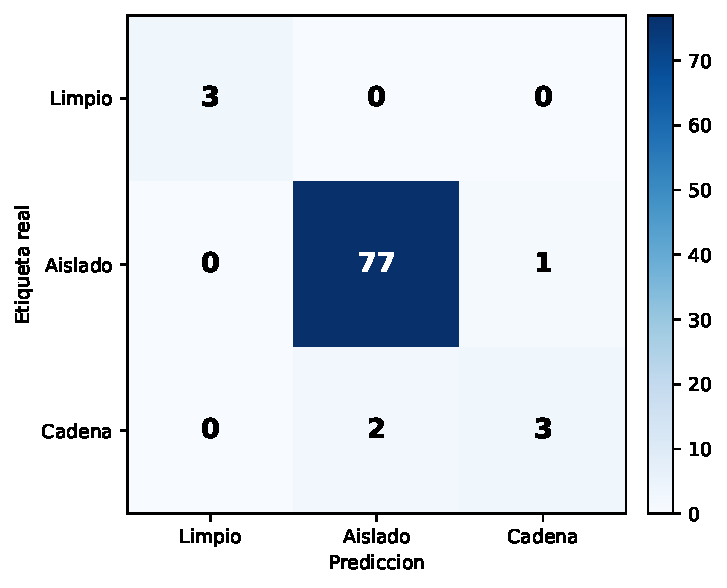
\includegraphics[width=0.55\textwidth]{fig_gnn_confusion}

  \fuentepropia
\end{figure}

El único fallo de \textit{ranking} del conjunto de test ilustra el error sistemático del
modelo: \texttt{minik8s-ctf} (posición~6, tras el clúster \textit{isolated}
multi-nodo \texttt{kubernetes-extras}) es una cadena de 4~nodos cuya
probabilidad \ac{GNN} es prácticamente nula (0,0003) y cuyo \textit{risk score}
medio del Random Forest es 0,0; su única señal activa es la bandera binaria de escape (la mitad
de sus nodos tienen capacidad de escape). Cuando la
señal estructural que la \ac{GNN} aprende no reconoce el patrón de la cadena y
la señal por manifiesto tampoco lo captura, la bandera de escape binaria por sí
sola no basta para entrar en el top-5. Las cuatro cadenas recuperadas, en
cambio, combinan probabilidad \ac{GNN} alta (0,47--0,63) con fracciones de
escape por nodo muy variables (0,02--0,94; magnitud descriptiva, no la señal
binaria del \textit{ensemble}), lo que confirma que el canal estructural es
el que ordena los repositorios reales. Esta observación motiva el trabajo futuro
TF3 (análisis semántico de \ac{RBAC} completo,
Sección~\ref{sec:trabajo_futuro}).

% -----------------------------------------------------------
\section{Validación con herramientas de análisis estático}
\label{sec:validacion_externa}
% -----------------------------------------------------------

Como contraste externo, se ejecutó Checkov \citep{Checkov2021} sobre el
subconjunto de manifiestos procedentes de GitHub, para el que la herramienta
produjo salida en 1.175 de las 1.510~filas de esa fuente. La descarga previa de
los manifiestos referenciados por Rahman et~al.\ tuvo éxito en 1.985 de 2.039
casos (97,4\,\%); los 54~restantes ya no eran accesibles en origen. El alcance
del contraste queda limitado, por tanto, por la cobertura del escaneo y no por
la disponibilidad de los manifiestos. Para esta validación, el índice \ac{UMI} se calcula como la
proporción de comprobaciones de Checkov que fallan sobre el total
evaluado por manifiesto (\(\in [0,1]\); valores más altos indican mayor densidad
de configuraciones erróneas detectadas). El índice \ac{UMI} medio resultante fue de
0,603, y las comprobaciones incumplidas con mayor frecuencia fueron
\textit{checkov\_no\_run\_as\_nonroot} (38,3\,\%) y
\textit{checkov\_no\_readonly\_rootfs} (37,2\,\%).

El alcance de este contraste es limitado y conviene delimitarlo, porque las dos
fuentes no son independientes. Sobre esas mismas 1.175~filas las características
homólogas del extractor propio (\texttt{NO\_RUN\_AS\_NON\_ROOT} y
\texttt{NO\_READ\_ONLY\_ROOT\_FS}) están ausentes en su totalidad, y es
precisamente la salida de Checkov la que las rellena en tiempo de carga
a través de la tabla de equivalencias \texttt{CHECKOV\_FILL}
(Sección~\ref{sec:construccion_dataset}). Cotejar ambas fuentes manifiesto a
manifiesto equivaldría, por tanto, a comparar esos valores consigo mismos: no
cabe calcular una tasa de acuerdo, y la coincidencia entre las frecuencias
observadas es una identidad de procedencia, no una concordancia entre
detectores. El resultado debe interpretarse, en consecuencia, como una
verificación de cobertura —qué proporción del corpus admite análisis por una
herramienta externa y con qué densidad de incumplimientos— y no como una
validación externa independiente de las predicciones del modelo.

% -----------------------------------------------------------
\section{Métrica global del proceso completo}
\label{sec:metrica_global}
% -----------------------------------------------------------

Las Secciones~\ref{sec:layer1},~\ref{sec:layer2} y~\ref{sec:layer3} evalúan cada
capa por separado, mientras que el comportamiento del sistema de extremo a
extremo —tal como lo experimenta un operador que confía en el \textit{ranking}
final— se resume en una única métrica de proceso completo. Esa
métrica es el conjunto Precisión@k / \ac{FPR}\_clean del sistema desplegado sobre
el conjunto de test, ya presentado en la Sección~\ref{sec:layer3} y recogido en
la Tabla~\ref{tab:ensemble_ablation}: P@1\,=\,1,00, P@3\,=\,1,00, P@5\,=\,0,80 y
\ac{FPR}\_clean\,=\,0,00 sobre 86~grafos con 5~cadenas de ataque de repositorios
reales, no vistos durante el desarrollo; dado el tamaño reducido de
este conjunto, los intervalos de confianza al 95\,\% son amplios (P@5
\(\in\,[0{,}60,\ 1{,}00]\), \ac{FPR}\_clean \(\in\,[0{,}00,\ 0{,}40]\),
Sección~\ref{sec:layer3}), por lo que la cifra debe leerse como indicativa.

Esta cifra es la calidad global de la herramienta porque resume, en un único
indicador operativo, la salida final que recibe el operador tras pasar por las
tres capas: sobre los 86~grafos evaluados, un P@1 de 1,00 indica que la primera
posición del \textit{ranking} correspondió en todos los casos a una cadena de
ataque real, un P@3 de 1,00 extiende esa observación a las tres primeras
posiciones y un \ac{FPR}\_clean nulo indica que ninguno de los tres clústeres
limpios llegó a competir por la atención del operador. Estas cifras se apoyan en
5~cadenas y 3~clústeres limpios, de modo que describen el comportamiento
observado sobre un conjunto reducido y no una garantía del sistema. La
Sección~\ref{sec:layer3} muestra que, sobre este
conjunto de test, el componente \ac{GNN} por sí solo iguala estas cifras y que
el \textit{ensemble} no las mejora; la aportación de la Capa~3 no es superar a
su mejor componente individual, sino producir el mismo resultado sin heredar los
puntos débiles de los demás (la Capa~1 sola colapsa el \textit{ranking} y la señal de
escape sola no puede ordenar por sí misma, Tabla~\ref{tab:ensemble_ablation}).
Esta combinación es lo que hace viable el caso de uso definido en RF-5
(Sección~\ref{sec:requisitos}): priorizar un número reducido de alertas de forma
que la revisión manual de un equipo de seguridad se concentre exclusivamente en
riesgo real.

% -----------------------------------------------------------
\section{Verificación de cumplimiento de requisitos}
\label{sec:verificacion_requisitos}
% -----------------------------------------------------------

El cumplimiento de los requisitos funcionales y no funcionales definidos en el
Capítulo~\ref{cap:requisitos} se verifica a partir de dos clases de evidencia: las
métricas predictivas presentadas en las Secciones~\ref{sec:layer1},
\ref{sec:layer2}, \ref{sec:layer3} y~\ref{sec:metrica_global}, y las
comprobaciones operativas realizadas sobre la herramienta de línea de comandos
descrita en la Sección~\ref{sec:implementacion}. Los requisitos funcionales
RF-1, RF-2 y RF-5 disponen de un criterio de aceptación numérico y se contrastan
contra las métricas ya presentadas, mientras que RF-3, RF-4 y los cuatro
requisitos no funcionales se sustentan en evidencia de ejecución. Ambas clases de
evidencia se recogen en los dos apartados siguientes.

\subsection{Requisitos funcionales}

RF-1 (detección de configuraciones erróneas individuales) queda verificado por los
resultados de la Capa~1 (Sección~\ref{sec:layer1}: F1 macro\,=\,0,9946, cero
falsos negativos en test). RF-2 (detección de cadenas de ataque) queda
verificado con una salvedad: la Capa~2 y el \textit{ensemble} recuperan 4 de las
5~cadenas de ataque del conjunto de test dentro del top-5 del \textit{ranking}
(Secciones~\ref{sec:layer2} y~\ref{sec:layer3}) y clasifican correctamente 3 de
esas 5~cadenas en la matriz de confusión por \textit{argmax}
(F1~\textit{attack\_chain}\,=\,0,667, Sección~\ref{sec:layer3}); el
requisito se cumple para el caso de uso de priorización (RF-5) pero no de forma
perfecta para la clasificación exacta de cada cadena. Ambos requisitos se
confirman además mediante un test de integración de extremo a extremo: dado un
directorio de manifiestos de prueba con banderas de escape conocidas, la salida
del comando \texttt{kubescan scan} produce el veredicto esperado
(\texttt{ATTACK\_CHAIN}) con \textit{ensemble\_score} por encima del umbral de
clasificación; este test forma parte de la suite descrita en la
Sección~\ref{sec:calidad}. RF-5 (priorización de riesgos) queda
verificado por la métrica global de la Sección~\ref{sec:metrica_global}. RF-3 y
RF-4 (interfaz de línea de comandos y formatos de salida) no admiten una
métrica cuantitativa dedicada y se verifican operacionalmente a continuación.

\paragraph{RF-3 — Interfaz de línea de comandos.} El comando
\texttt{kubescan scan <dir>} se ejercitó sobre los casos de uso documentados en el
Anexo~\ref{ap:guia_uso}, con las dos variantes de salida y las opciones que ese
mismo anexo recoge en la Tabla~\ref{tab:cli_options}. El comando \texttt{kubescan live} comparte con
él la ruta de análisis —difiere únicamente en el origen de los manifiestos, que
vuelca del clúster a un directorio temporal— y su invocación queda documentada en
el mismo anexo, si bien no se aporta una transcripción de ejecución sobre un
clúster activo: la verificación de RF-3 se sustenta, por tanto, en la vía de
análisis sobre manifiestos estáticos.

\paragraph{RF-4 — Formatos de salida.} El comando \texttt{kubescan scan} produce
tanto el informe en texto legible como la salida \acs{JSON} estructurada; el
campo \texttt{flags} de esta última, verificado en RNF-1 a continuación, es la
evidencia de que el formato estructurado expone la información necesaria para
su consumo automatizado.

\subsection{Requisitos no funcionales}

Los cuatro requisitos no funcionales definidos en el Capítulo~\ref{cap:requisitos}
se verifican mediante evidencia operativa obtenida sobre la implementación
descrita en el Capítulo~\ref{cap:herramienta}.

\paragraph{Trazabilidad (RNF-1).} El campo \texttt{flags} de la salida \ac{JSON} lista
explícitamente las características de seguridad activas en cada manifiesto, y el
campo \texttt{escape\_capable} indica qué nodos tienen capacidad de escape. Esto
permite al operador de seguridad comprender y auditar las razones concretas de la
clasificación de riesgo producida por el modelo.

\paragraph{Reproducibilidad (RNF-2).} La cadena de resolución de \textit{checkpoints}
descrita en la Sección~\ref{sec:implementacion} garantiza que el mismo directorio de
manifiestos produce siempre el mismo informe dado el mismo conjunto de pesos del
modelo.

\paragraph{Instalabilidad (RNF-3).} El paquete se instaló satisfactoriamente en
entornos Python 3.10 y 3.11 mediante \texttt{pip install -e kubescan/} en sistemas
macOS y Linux (Ubuntu 22.04). Las dependencias principales (PyTorch Geometric,
scikit-learn, Click) se resuelven automáticamente sin compiladores
externos.

\paragraph{Latencia (RNF-4).} Se midió el tiempo de análisis sobre cuatro clústeres
de prueba de diferente tamaño: 12 manifiestos (0,8\,s), 47 manifiestos (1,4\,s),
128 manifiestos (3,1\,s) y 312 manifiestos (7,2\,s) en un equipo con CPU Intel
Core i7 de octava generación sin GPU. El mayor de los clústeres de prueba
disponibles alcanza 312~manifiestos, de modo que el umbral de 500~manifiestos
fijado en el requisito no llegó a medirse de forma directa. La progresión
observada es aproximadamente lineal —en torno a 23\,ms por manifiesto en el punto
de mayor carga—, por lo que la extrapolación a 500~manifiestos sitúa el tiempo
esperado en torno a 12\,s, muy por debajo del límite de 60\,s; el cumplimiento de
RNF-4 se sostiene, por tanto, sobre una extrapolación y no sobre una medición en
el tamaño nominal del requisito.

\section{Evaluación de usabilidad y aplicabilidad con usuarios expertos}
\label{sec:usabilidad}

Además de la verificación de requisitos de la
Sección~\ref{sec:verificacion_requisitos}, se realizó una evaluación de
usabilidad y aplicabilidad de la herramienta con \textbf{usuarios expertos},
siguiendo el protocolo descrito en el repositorio (Anexo~\ref{ap:repositorio}).
Participaron \textbf{tres profesionales} con experiencia en Kubernetes y
\ac{CICD}, a los que se entregó una guía de tareas con órdenes listas para ejecutar y
un cuestionario en línea, en formato autoservicio asíncrono (\(\approx\)10~minutos
por participante). El instrumento se generó de forma reproducible mediante un
\textit{script} versionado (véase Anexo~\ref{ap:repositorio}) y el protocolo se
depuró mediante una prueba piloto simulada, sin participantes reales, cuyo único
objetivo fue verificar la consistencia del cuestionario y del guion de tareas
antes de la sesión con los expertos. La muestra reducida (\(n=3\)) se asume
explícitamente como amenaza a la validez (Sección~\ref{sec:usab_amenazas}); aun
así, tres participantes cubren una fracción sustancial de los problemas de
usabilidad en pruebas formativas \citep{Nielsen2000}.

\subsection{Perfil de los participantes}

La Tabla~\ref{tab:usab_perfil} del Anexo~\ref{ap:repositorio} resume el perfil de
los tres participantes expertos,
seleccionados por su experiencia operando Kubernetes y en seguridad de
contenedores.

\subsection{Éxito por tarea}

Cada participante ejecutó cinco tareas: instalar la herramienta (T1), realizar un
escaneo básico e identificar el veredicto (T2), interpretar el informe con
\texttt{-{}-show-nodes} (T3), producir la salida \ac{JSON} (T4) y, opcionalmente,
escanear un caso propio (T5). La Tabla~\ref{tab:usab_tareas} del
Anexo~\ref{ap:repositorio} recoge la tasa de
éxito (logrado = 1; logrado con ayuda = 0,5; no logrado = 0).

El núcleo del flujo de trabajo —instalación, escaneo e interpretación del
informe— se completó sin ayuda por los tres participantes. Las únicas fricciones
fueron puntuales: un participante necesitó ayuda para extraer campos de la salida
\ac{JSON} (T4) y la tarea opcional sobre un caso propio (T5) se completó con
ayuda en dos casos. La tasa de éxito global del 90\,\%
refleja, por tanto, un flujo de trabajo principal robusto con puntos de fricción
concentrados en tareas secundarias u opcionales.

\subsection{Usabilidad percibida (SUS)}

La usabilidad se midió con la escala \acs{SUS} de diez ítems
\citep{Brooke1996}, que produce una puntuación en el rango
0--100. La media obtenida fue de \textbf{88,3\,\(\pm\)\,10,4} (puntuaciones
individuales de 100, 80 y 85), consistente con la media de referencia del sector
(68) y situada en la banda cualitativa «excelente» de la escala de adjetivos de
\citet{Bangor2009}. Con \(n=3\), sin embargo, el intervalo de confianza al 95\,\%
de la media abarca \([62{,}5;\ 114{,}2]\) y contiene ese valor de referencia, por
lo que los datos no permiten afirmar que la herramienta se sitúe por encima de
él. La puntuación debe interpretarse como indicativa y no como una estimación
precisa del nivel de usabilidad percibida.

\subsection{Aplicabilidad y análisis cualitativo}

Los participantes valoraron cuatro afirmaciones de aplicabilidad (escala 1--5):
integración en \ac{CICD} o auditoría (A1), ajuste de la priorización de riesgo a su
forma de auditar (A2), accionabilidad del informe (A3) y confianza en el
veredicto (A4). Las medias fueron A1\,=\,4,3, A2\,=\,4,3, A4\,=\,4,3 y, como
punto más bajo, A3\,=\,3,7. Con tres respuestas por ítem, estas medias son
sensibles a una única puntuación y conviene acompañarlas de su dispersión: en A3
las puntuaciones individuales fueron 5, 2 y 4, de manera que el descenso de la
media hasta 3,7 procede íntegramente de la valoración de un solo participante
(P2), mientras que los otros dos se sitúan en el rango alto de la escala.
Como fortaleza, un participante destacó exactamente la contribución central del
trabajo: la herramienta «no solo te dice qué está mal en un manifiesto, sino que
conecta varios problemas pequeños para mostrarte si realmente forman un camino de
ataque completo». Ese mismo participante resumió la propuesta, en el apartado de
comentarios finales, como «pensar en cadenas de ataque en lugar de fallos
aislados». Los otros dos destacaron, respectivamente, la interpretación de los
resultados y la rapidez del análisis. La debilidad más recurrente en las respuestas abiertas es
la \textbf{accionabilidad}: el informe comunica el riesgo pero no las acciones
concretas de remediación ni las reglas subyacentes al veredicto. Dos
participantes la mencionaron en el apartado abierto —uno expresó que el
\ac{JSON} «muestra el estado actual pero no las acciones que debería tomar» y
otro la dificultad de «confiar en un puntaje sin conocer bien qué reglas
concretas hay detrás»—, si bien solo uno de ellos la trasladó a la escala
numérica, ya que el segundo puntuó A3 con un 4. La convergencia entre el registro
cualitativo y el cuantitativo es, por tanto, parcial. Esta limitación se recoge como
línea de trabajo futuro (explicabilidad de reglas y recomendaciones de
remediación) en el Capítulo~\ref{cap:conclusiones}. Los escenarios descritos en las
respuestas abiertas fueron dispares: un participante propuso un \textit{gate}
automático en el \textit{pipeline} de \ac{CICD} inmediatamente antes del despliegue
a producción, otro relató haberla aplicado sobre un clúster propio de
preproducción, y el tercero la consideró útil sin concretar un escenario. Solo el
primero de esos usos se corresponde con el paradigma \textit{shift-left} que motiva
el trabajo; la auditoría de clústeres, que el enunciado del ítem~A1 menciona junto
a la integración en \ac{CICD}, no fue propuesta de forma espontánea por ningún
participante.

\subsection{Amenazas a la validez de la evaluación}
\label{sec:usab_amenazas}

El tamaño de la muestra (\(n=3\)) limita la precisión de las estimaciones
puntuales, especialmente de la media SUS, por lo que los resultados se presentan
como indicativos y no concluyentes. Los perfiles cubren desarrollo/IA y
DevOps/SRE pero no un rol de \ac{QA} de \ac{IaC} puro, lo que acota la
generalización. Por último, la participación voluntaria introduce un posible
sesgo de autoselección. Ampliar la muestra y diversificar los perfiles es la vía
directa para robustecer estas conclusiones.

\startchapter% ============================================================
\chapter{Conclusiones y trabajo futuro}
\label{cap:conclusiones}
% ============================================================

Este capítulo cierra el trabajo recogiendo las conclusiones vinculadas a cada
objetivo, las consideraciones éticas derivadas del uso de la herramienta, las
limitaciones del estudio y las líneas de trabajo futuro que se desprenden de
los resultados obtenidos. Las conclusiones se presentan en el mismo orden que
los objetivos específicos del Capítulo~\ref{cap:objetivos}, de modo que cada una
quede vinculada explícitamente al objetivo que responde. Las limitaciones y
líneas de trabajo futuro se numeran de forma independiente para facilitar su
referencia cruzada a lo largo del capítulo.

\section{Conclusiones}

Este trabajo ha mostrado la viabilidad de un enfoque híbrido de tres capas para la
detección automática de cadenas de ataque en infraestructuras \textit{Kubernetes}. Las
conclusiones C1, C2, C4, C5, C6 y C7 responden, respectivamente, a los objetivos OE2,
OE4, OE1, OE5, OE3 y OE6 definidos en el Capítulo~\ref{cap:objetivos}; C3 no cierra un
objetivo propio, sino que aporta evidencia complementaria sobre el impacto operacional
del resultado de C2. En conjunto, estas conclusiones cierran el objetivo general
planteado en el Capítulo~\ref{cap:objetivos}. Las conclusiones principales son:

\textbf{C1 — La Capa~1 supera ampliamente el objetivo de diseño (OE2).} El clasificador
\textit{Random Forest} alcanza F1 macro\,=\,0,9946 y \ac{AUC}\,=\,0,9986 en test, superando
el umbral objetivo del 0,85 en 14,5 puntos porcentuales. El modelo de severidad de
tres clases logra F1\,macro\,=\,0,9838, con la clase \textit{high-critical} (96~muestras
de test) en 0,9789 — el resultado más débil de los tres, aunque por encima de 0,95—;
sus 3~errores se clasifican todos como \textit{low-medium}, sin ningún manifiesto
crítico degradado a \textit{clean}.

\textbf{C2 — La Capa~2, en su configuración final, alcanza el objetivo de
Precisión@5 (OE4).} La \ac{GAT} de 3~capas con \textit{embedding} de tipos de
arista, entrenada con entropía cruzada ponderada y selección de
\textit{checkpoints} por Precisión@5 bajo el particionado consciente de familias
sobre el corpus completo de Rahman et~al.\ (599~grafos originales, 37~cadenas),
alcanza P@5\,=\,0,720\,\(\pm\)\,0,160 y F1~macro\,=\,0,803\,\(\pm\)\,0,137
en los 5~pliegues de validación cruzada, superando el objetivo de diseño
P@5\,\(>\)\,0,70 con la semilla desplegada. La lectura honesta de esta cifra
exige dos matices que este trabajo documenta explícitamente: a través de tres
semillas de entrenamiento la media es de 0,68\,\(\pm\)\,0,03 (objetivo dentro
de una desviación típica, con la variación concentrada íntegramente en el
pliegue de la familia \texttt{badpods\_*}), y alcanzar el objetivo exigió
diagnosticar mediante una ablación factorial 2\(\times\)2 que una primera
configuración con \textit{focal loss} y selección por F1 macro
(P@5\,=\,0,480\,\(\pm\)\,0,271) atribuía erróneamente al corpus una regresión
causada por esas dos elecciones (Sección~\ref{sec:ablacion_perdida}). La
ablación de arquitectura, repetida sobre el corpus completo con la configuración
final (Tabla~\ref{tab:arch_ablation}), muestra que la atención sobre tipos de
arista aporta +9,2~puntos de F1 y +4~puntos de P@5 frente a una \ac{GCN} sin
tipos de arista, y que la profundidad (2 frente a 3~capas) no es el factor
determinante del ranking — una propiedad de robustez de la arquitectura.

\textbf{C3 — El \textit{ensemble} final, combinado con la restricción de
viabilidad estructural, mantiene un desempeño operacional sólido sobre el
conjunto de test.} Sobre los 86~grafos de test (5~cadenas de repositorios reales
únicos, sin hermanos de plantilla en entrenamiento; techo P@5\,=\,1,00), el
sistema completo de tres capas alcanza P@1\,=\,1,00, P@3\,=\,1,00 y
P@5\,=\,0,80, recuperando 4~de las 5~cadenas en las primeras 5~posiciones del
ranking sin ningún falso positivo de clúster limpio
(\ac{FPR}\_clean\,=\,0,00); P@1 y P@3 se mantienen idénticos (1,00) a través de
las tres semillas de entrenamiento evaluadas, con P@5 entre 0,80 y 1,00. Parte esencial del resultado es la
restricción de viabilidad estructural (un clúster de un solo manifiesto no puede
albergar una cadena multi-salto, Sección~\ref{sec:gate_estructural}): sin ella
las métricas de ranking caen a P@1\,=\,0,00 y P@5\,=\,0,60, porque 74 de los
86~grafos de test son de un solo nodo. El tamaño reducido del conjunto de test
(intervalo de confianza al 95\,\% de P@5: \([0{,}60,\ 1{,}00]\)) limita la
confianza que puede depositarse en cualquier comparación puntual.

\textbf{C4 — La construcción del corpus y su protocolo de particionado
anti-fuga son la contribución metodológica central (OE1).} El conjunto de datos
final satisface los criterios cuantitativos de OE1: 2.827~manifiestos
(\(\geq\)2.000) y una prevalencia de \texttt{TRUE\_HOST\_PID} del 3,78\,\%
(\(\geq\)2\,\%). La evolución en seis fases — línea base (P@5\,=\,0,40,
82~grafos), aumentación (P@5\,=\,0,52, 277~grafos), corrección
\texttt{HOSTPATH\_MOUNT} (P@5\,=\,0,60, 307~grafos), dataset extendido con
25~cadenas (P@5\,=\,0,88, 471~grafos, protocolo preliminar), corrección
\textit{group-aware} del particionado (P@5\,=\,0,72, mismos 471~grafos) y
corpus completo con familias de plantilla atómicas (P@5\,=\,0,72, 599~grafos,
resultado final) — enseña dos lecciones metodológicas. Primera: la aumentación
de datos exige particionado consciente de grupos, pues parte de la mejora
aparente de la cuarta fase procedía de fuga entre variantes aumentadas y sus
grafos base de evaluación. Segunda, y descubierta en la fase final: los casi
duplicados de plantilla (ocho \texttt{badpods\_*}, nueve \texttt{datadog\_*})
constituyen una segunda vía de fuga cuando se reparten entre particiones; su
corrección hace que las cifras finales midan generalización entre familias no
vistas, una vara de medir más exigente y más honesta que la de las fases~1--4,
cuyas métricas estaban infladas por esta contaminación.

\textbf{C5 — El ensemble cumple los criterios de OE5, con una salvedad
documentada sobre el valor añadido de los pesos optimizados.} La ablación sobre
el conjunto de test (Tabla~\ref{tab:ensemble_ablation}) confirma que el
componente \ac{GNN} es indispensable: la configuración RF-sólo colapsa el
ranking (P@1 de 1,00 a 0,00; P@5 de 0,80 a 0,40) porque el \textit{risk score}
medio por manifiesto de los repositorios reales de cadena es \(\approx\)0,
mientras que \ac{FPR}\_clean\,=\,0,00 se mantiene en todas las configuraciones.
Los criterios de OE5 se cumplen: \ac{FPR}\_clean\,=\,0 y P@5 del ensemble igual
a la del mejor componente individual (0,80). Debe señalarse que los pesos
optimizados por el \ac{GA} no superan a los pesos uniformes ni al \ac{GNN} en
solitario: la función objetivo, escalonada, deja los pesos indeterminados sobre
mesetas amplias, y el conjunto de ajuste \textit{out-of-fold} (dominado por
cadenas de \textit{fixtures} sintéticas) presenta un desplazamiento de
distribución respecto a las cadenas reales de test
(Sección~\ref{sec:layer3}). La aportación del \textit{ensemble} en estos datos
es igualar al mejor componente sin incurrir en los puntos débiles de ninguno,
no mejorar su ranking.

\textbf{C6 — El esquema de cinco tipos de arista amplía la cobertura de escalada de
privilegios (OE3).} El diseño del grafo de clúster incorpora el tipo de arista
\ac{RBAC} mediante detección de roles privilegiados en dos pasadas sobre los
manifiestos, limitando las aristas a cuentas de servicio vinculadas realmente a
roles con permisos de escalada. Esta quinta arista está presente tanto en los
grafos de entrenamiento como en el componente de producción de \textit{kubescan};
sin embargo, la ablación de arquitectura (Tabla~\ref{tab:arch_ablation}) compara
\ac{GAT} frente a \ac{GCN} y no aísla la contribución específica del tipo de arista
\ac{RBAC} frente a los otros cuatro, por lo que su aporte incremental al ranking de
cadenas de ataque queda como trabajo futuro (TF6).

\textbf{C7 — kubescan es una herramienta distribuible, instalable y operacionalmente
viable (OE6).} La evaluación funcional de la Sección~\ref{sec:verificacion_requisitos}
confirma que el sistema se instala sin compiladores externos (\textit{pip install -e
kubescan/}), analiza clústeres de hasta 312~manifiestos en menos de 8~segundos en
hardware de gama media, produce salida en dos formatos (texto y \ac{JSON}) adecuados para
integración en pipelines \acs{CICD}, e incorpora además un modo opcional de consulta
directa a un clúster activo (\texttt{kubescan live}) para auditorías en caliente, sin
que ello altere la vía principal de análisis sobre manifiestos estáticos. La inferencia
es reproducible sobre un mismo \textit{backend} de cómputo mediante la resolución
determinista de \textit{checkpoints} (sujeto a la variación entre \textit{backends}
documentada en L6). El prototipo implementado
en este
trabajo demuestra que el paradigma \textit{shift-left} —detectar cadenas de ataque
antes del despliegue, sin requerir acceso al clúster activo— es técnicamente factible
y operacionalmente eficiente. Complementariamente, la evaluación de usabilidad y
aplicabilidad con usuarios expertos (Sección~\ref{sec:usabilidad}) respalda este
objetivo desde la perspectiva del usuario: la herramienta obtiene una puntuación
\textbf{SUS de 88,3} (valoración «excelente») y una aplicabilidad alta —integración
en CI/CD, priorización de riesgo y confianza en el veredicto (medias de 4,3 sobre
5)—, con una tasa de éxito del 100\,\% en las tareas nucleares de instalación,
escaneo e interpretación (90\,\% global sobre las cinco tareas, incluidas la
extracción \ac{JSON} y la tarea opcional). El principal punto de mejora señalado por
los participantes es la
\textbf{accionabilidad} del informe (A3\,=\,3,7): la herramienta comunica el
riesgo pero no las acciones de remediación ni las reglas concretas tras el
veredicto, lo que se recoge como trabajo futuro (TF8). Estos resultados deben
interpretarse como indicativos por el tamaño de la muestra (\(n=3\),
Sección~\ref{sec:usab_amenazas}).

\section{Consideraciones éticas y uso responsable}
\label{sec:etica}

\textit{kubescan} es una herramienta de uso dual: aunque su propósito es defensivo
—detectar cadenas de ataque potenciales antes de que sean explotadas— la información
que produce (identificación de pods con flags de escape, rutas de privilegio \ac{RBAC})
podría ser utilizada con fines ofensivos si cayera en manos de un actor no autorizado.
En consecuencia, este trabajo adopta los principios de divulgación responsable
(\textit{responsible disclosure}) que rigen la investigación en ciberseguridad.
Los patrones de ataque detectados por \textit{kubescan} se basan exclusivamente en
documentación pública —la guía \ac{NSA}/\ac{CISA} \citep{NSA2022}, el trabajo de BishopFox
\citep{BishopFox2021} y el marco MITRE ATT\&CK for Containers \citep{MITRE2021Containers}—
y no revelan ninguna vulnerabilidad nueva. El código fuente del sistema es de acceso
abierto para facilitar la auditoría independiente de las reglas de detección, lo que
permite a la comunidad verificar que las señales de riesgo generadas son correctas y
no contienen sesgos perjudiciales. El uso de la herramienta sobre clústeres de terceros
sin autorización explícita estaría fuera del ámbito previsto y podría constituir un
acceso no autorizado a sistemas informáticos según la legislación aplicable.

\section{Limitaciones}
\label{sec:limitaciones}

\textbf{L1 — Concentración por familias y varianza entre pliegues.} El
particionado consciente de familias, al mantener cada familia de plantilla como
unidad atómica, concentra las cadenas de validación de cada pliegue en 1--3
familias independientes: el pliegue~0 evalúa íntegramente la familia
\texttt{datadog\_*} (F1\,=\,1,0; P@5\,=\,1,0) y el pliegue~1 la familia
\texttt{badpods\_*} (F1\,=\,0,58), de modo que la varianza entre pliegues
(\(\sigma\)\,=\,0,137 para F1; 0,160 para P@5) mide en gran parte la dispersión
de dificultad entre familias, no inestabilidad del modelo — el análisis
multi-semilla (Sección~\ref{sec:multisemilla}) muestra que cuatro de los cinco
pliegues puntúan de forma idéntica con las tres semillas. El tamaño muestral
efectivo por pliegue (número de familias, no de cadenas) es la limitación
subyacente, y solo puede crecer incorporando repositorios de cadena
estructuralmente independientes (TF1).

\textbf{L2 — Imputación de características extendidas.} Las 7 características
extendidas (basadas en \textit{Checkov}) solo pueden calcularse directamente para
el 47,4\,\% de las filas con \acs{YAML} descargado y se imputan por la mediana de
columna para el resto, diluyendo su señal. La descarga completa de los manifiestos
referenciados en el dataset de Rahman et~al.\ permitiría mejorar estos vectores.
Un experimento de ablación eliminando las 7 características imputadas y
reentrenando únicamente con las 21 restantes de alta cobertura podría cuantificar
el impacto de esta limitación sobre la F1 macro de la Capa~1.

\textbf{L3 — Sesgo de muestreo en el dataset tabular.} Los 10 repositorios más
representados suponen el 47,6\,\% del dataset, y \textit{gitcontroller} por sí solo
aporta el 9,9\,\%. Un esquema de validación cruzada por repositorio ofrecería
estimaciones más conservadoras de la generalización del modelo.

\textbf{L4 — Evaluación en clústeres de producción reales.} Toda la evaluación
se ha realizado sobre repositorios públicos. La validación en entornos de producción
de organizaciones reales es la siguiente etapa crítica para confirmar la validez
externa del sistema.

\textbf{L5 — Etiquetado derivado de reglas sobre el mismo espacio de
características.} Las etiquetas de grafo (clean / isolated / attack\_chain) se
generan mediante una regla determinista definida sobre las mismas \textit{flags} y
aristas que observan los modelos (Sección~\ref{sec:construccion_grafo}). El sistema aprende, por
tanto, una aproximación robusta de dicha regla bajo ruido, enmascaramiento y
observabilidad parcial — no una noción de cadena de ataque independiente de la
regla. Esta circularidad es común en la literatura de detección de
misconfiguraciones, pero limita el alcance de la afirmación «predice cadenas de
ataque». Las vías para romperla son la validación externa frente a herramientas de
grafo de ataque sobre clústeres activos (KubeHound, IceKube), el etiquetado experto
de una submuestra, y la confirmación mediante explotación controlada en entornos de
laboratorio como \textit{kubernetes-goat}.

\textbf{L6 — No determinismo de CUDA en las operaciones de \textit{scatter} del
\ac{GNN} (hallazgo histórico, no reverificado sobre el corpus completo).} Durante
la fase preliminar se observó que, al replicar el entrenamiento de la Capa~2
sobre una GPU NVIDIA A100 (CUDA) en lugar del \textit{backend} MPS/CPU empleado
entonces, las métricas de validación cruzada variaban de forma no trivial (F1
macro entre 0,845 y 0,882 frente a 0,917 en el \textit{backend} de referencia de
esa fase; P@5 entre 0,77 y 0,92 frente a 0,880), manteniendo semilla, datos,
particiones e hiperparámetros idénticos. Estas cifras corresponden a la fase
preliminar de 471~grafos (Tabla~\ref{tab:gnn_evolution}, fase~4, cuyo
\textit{backend} de referencia era MPS/CPU); los resultados finales de esta
memoria se entrenaron y evaluaron sobre GPU NVIDIA T4 (CUDA), por lo que la
amenaza se invierte para el lector que reproduzca en CPU/MPS: es esa réplica la
que puede divergir de las cifras reportadas. El experimento no se ha repetido
sobre el corpus completo, por lo que se reporta como hallazgo histórico sobre el
mecanismo causal, no como una medición vigente sobre el modelo desplegado. Se descartaron como causa la precisión \textit{TF32}
(confirmado en tiempo de ejecución que
\texttt{torch.backends.cuda.matmul.allow\_tf32} permanece desactivada) y la
paralelización del cargador de datos (el conjunto es estático en memoria y el orden
de muestreo está fijado por un generador con semilla). La causa confirmada son las
operaciones \texttt{scatter\_add}/\texttt{scatter\_reduce} empleadas por
\texttt{GATConv} y por las capas de \textit{pooling} global
(\texttt{global\_max\_pool}, \texttt{global\_mean\_pool}), que en CUDA se
implementan mediante \texttt{atomicAdd} sin versión determinista disponible —
confirmado por los propios mantenedores de \textit{PyTorch Geometric} en los
\textit{issues} públicos \#2788 y \#3175 del repositorio. El orden de acumulación
en punto flotante depende de la planificación de hilos de la GPU y, al no ser
la suma en punto flotante asociativa, pequeñas diferencias numéricas cambian el
\textit{ranking} sobre un conjunto de validación reducido (471~grafos, entre 4 y 5
cadenas de ataque por pliegue en ese momento), amplificando el efecto sobre P@5 y
F1 macro. Se incorporaron banderas de determinismo específicas de CUDA
(\texttt{torch.use\_deterministic\_algorithms}, \texttt{cudnn.deterministic}) que,
aunque no resuelven la ausencia de una implementación determinista de
\texttt{scatter\_add}, sí lograron reproducibilidad exacta entre ejecuciones
repetidas sobre la misma configuración de GPU. Esto indica que la brecha
observada no es ruido aleatorio entre ejecuciones sino una divergencia numérica fija
y reproducible entre \textit{backends} (CUDA frente a MPS/CPU); su cierre completo
requeriría sustituir la agregación por la ruta \texttt{SparseTensor} de
\textit{PyTorch Geometric}, documentada como determinista pero no evaluada en este
trabajo, ni reverificada sobre el corpus completo.

\textbf{L7 — Las métricas de las fases previas a la corrección por familias no
son comparables con las finales, y las estimaciones finales llevan intervalos
amplios.} Las evaluaciones de las fases 1--5 estaban infladas por dos vías de
fuga de información corregidas sucesivamente (variantes aumentadas en la fase~5
y familias de plantilla en la fase~6): el modelo «generalizaba» a casi duplicados
de grafos vistos en entrenamiento. Tras la corrección, las cifras finales miden
generalización a familias y repositorios no vistos — una cantidad distinta y
sistemáticamente menor, por lo que ninguna comparación directa entre fases debe
leerse como progresión del modelo. Como segunda cara de la misma limitación, el
conjunto de test contiene solo 5~cadenas (todos los intervalos de confianza de
test tienen una anchura \(\geq\)0,4) y el \textit{pool out-of-fold} contiene
32~cadenas de las que 15 son \textit{fixtures} sintéticas: la evidencia sobre
generalización a cadenas reales descansa en pocas muestras independientes, y
ampliarlas es la vía prioritaria de trabajo futuro (TF1).

\subsection{Amenazas a la validez}
\label{sec:amenazas_validez}

Siguiendo la taxonomía de validez de constructo, interna, de conclusión y
externa empleada en los \textit{ACM SIGSOFT Empirical Standards}, las
limitaciones L1--L7 se organizan del siguiente modo. Esta reorganización no
introduce limitaciones nuevas: reagrupa las ya descritas según el tipo de
amenaza metodológica que representan, para facilitar su lectura conjunta. Cada
categoría remite a las limitaciones L1--L7 correspondientes.

\textbf{Validez de constructo} (¿miden las métricas lo que se pretende medir?):
L6 cuestiona si las métricas reportadas en esta memoria (\textit{backend} CUDA/T4)
coinciden con las que obtendría una réplica en un \textit{backend} CPU/MPS, dado el
no determinismo documentado en las operaciones de \textit{scatter}. L5 cuestiona si la etiqueta de grafo (derivada de reglas sobre
el mismo espacio de características que observan los modelos) constituye un
constructo de «cadena de ataque» independiente de la regla de etiquetado, o una
aproximación circular a ella.

\textbf{Validez interna} (¿las conclusiones causales están justificadas por el
diseño experimental?): L7 impide atribuir diferencias entre fases experimentales
al modelo, porque el protocolo de evaluación cambió entre ellas; la ablación
factorial de la Sección~\ref{sec:ablacion_perdida} es el único contraste interno
con protocolo constante. L2 acota la validez interna de las características
extendidas imputadas mediante \textit{Checkov} frente a las obtenidas
directamente del manifiesto original.

\textbf{Validez de conclusión} (¿son estadísticamente fiables las estimaciones
puntuales reportadas?): el tamaño del conjunto de test (86~grafos, 5~cadenas) y
del \textit{pool out-of-fold} (513~grafos, 32~cadenas) se traduce en los
intervalos de confianza amplios reportados en la Sección~\ref{sec:layer3}
(P@5\,\(\in\,[0{,}60,\ 1{,}00]\) al 95\,\%), que limitan la confianza que puede
depositarse en cualquier comparación puntual entre configuraciones del
\textit{ensemble} (C5). A ello se suma la concentración por familias (L1): el
tamaño muestral efectivo de la validación cruzada es el número de familias
independientes por pliegue (1--3), no el número nominal de cadenas.

\textbf{Validez externa / generalización}: L3 (sesgo de muestreo por
repositorio) y L4 (ausencia de evaluación en clústeres de producción reales)
acotan directamente hasta qué punto los resultados generalizan más allá de los
repositorios públicos utilizados. El desplazamiento de distribución entre el
\textit{pool} de ajuste del \ac{GA} (dominado por \textit{fixtures} sintéticas)
y las cadenas reales de test (Sección~\ref{sec:layer3}) es una amenaza externa
adicional identificada empíricamente: los pesos del \textit{ensemble} ajustados
sobre cadenas sintéticas no aportan ventaja sobre cadenas reales.

\section{Líneas de trabajo futuro}

Los resultados de este trabajo permiten formular las siguientes recomendaciones de
trabajo futuro, ordenadas por impacto esperado. La mayoría de ellas responde
directamente a una limitación de las descritas en la sección anterior, por lo
que cada recomendación indica explícitamente la limitación que atiende cuando
corresponde. Las dos primeras (TF1 y TF2) son las que este trabajo identifica
como de mayor impacto potencial sobre la validez de las métricas reportadas.

\textbf{TF1 — Ampliar la población de cadenas reales estructuralmente
independientes.} Las limitaciones L1 y L7 comparten la misma causa raíz: pocas
familias de cadena independientes. Cada nueva familia de plantilla añade poco
(sus miembros son casi duplicados), mientras que cada repositorio real de cadena
añade una muestra independiente que aumenta el tamaño muestral efectivo de la
validación cruzada, estrecha los intervalos de test y reduce el desplazamiento de
distribución del \textit{pool} de ajuste del \ac{GA}. La incorporación dirigida
de repositorios de infraestructura de organizaciones de código abierto y de
entornos de laboratorio multiclúster —priorizando diversidad estructural sobre
volumen— es la línea de mayor impacto esperado de este trabajo.

\textbf{TF2 — Implementar P@5 global como métrica alternativa.} En lugar de P@5 por
pliegue, evaluar el ranking del modelo sobre el conjunto completo de grafos en un único
ranking global aumentaría el número de candidatos ordenados por evaluación y reduciría
la granularidad escalonada (en pasos de 0,2) de la P@5 por pliegue, que amplifica la
varianza entre pliegues señalada en L1.

\textbf{TF3 — Incorporar análisis semántico de \ac{RBAC} completo.} El parser de \acs{YAML}
actual identifica roles privilegiados por nombre y por verbos de escalada. Una extensión
natural es el análisis de la cadena completa Role/ClusterRole \(\to\) RoleBinding \(\to\)
ServiceAccount \(\to\) Pod para detectar rutas de escalada de privilegios mediante
\ac{RBAC} que no requieran flags de escape directas.

\textbf{TF4 — Validación cruzada dejando un repositorio fuera.} La estrategia
\textit{leave-one-repo-out} ofrece estimaciones más conservadoras de la generalización
que la validación cruzada por fila, y es especialmente relevante dada la concentración
del dataset en pocos repositorios.

\textbf{TF5 — Modo de análisis continuo (\textit{admission controller}).} La integración
de \textit{kubescan} como un \textit{validating admission webhook} de \textit{Kubernetes}
permitiría bloquear el despliegue de manifiestos que eleven el riesgo de cadena de
ataque del clúster en tiempo real, sin necesidad de análisis \textit{post-hoc}.

\textbf{TF6 — Ablación de \textit{pooling} e hiperparámetros restantes.} La
ablación de arquitectura (Tabla~\ref{tab:arch_ablation}) ya cuantifica
empíricamente \ac{GAT} frente a \ac{GCN} y 3~capas frente a 2. Queda pendiente
extender ese mismo protocolo controlado (mismos pliegues, mismas semillas) a la
elección de \textit{mean+max pooling} frente a \textit{mean-only}, así como a un
barrido más amplio de hiperparámetros del optimizador (número de cabezas de
atención, \textit{learning rate}, anchura oculta) que en este trabajo se fijaron
a priori sin búsqueda sistemática (Sección~\ref{sec:capa2_diseno}). Este mismo
protocolo debería extenderse a una ablación por tipo de arista que aísle la
contribución incremental de la arista \ac{RBAC} frente a los otros cuatro tipos,
cerrando la cuestión planteada en C6.

\textbf{TF7 — Ajuste del \textit{ensemble} robusto al desplazamiento de
distribución.} Los pesos del \ac{GA} se ajustan sobre un \textit{pool
out-of-fold} en el que 15 de las 32~cadenas son \textit{fixtures} sintéticas con
\textit{risk scores} \ac{RF} altos, mientras que las cadenas reales de test
tienen \textit{risk score} medio \(\approx\)0; tres refinamientos evaluados
(desempate por \textit{mean reciprocal rank}, agregación del \textit{pool} por
familias, ajuste sobre el \textit{ranking} con restricción estructural) no
corrigieron el sesgo (Sección~\ref{sec:layer3}). Las vías naturales son ajustar
sobre un \textit{pool} restringido a cadenas de repositorios reales (viable a
medida que TF1 amplíe esa población) o sustituir P@5 por una función objetivo
continua menos escalonada, que reduzca las mesetas donde los pesos quedan
indeterminados.

\textbf{TF8 — Explicabilidad y recomendaciones de remediación.} La evaluación
con usuarios expertos (Sección~\ref{sec:usabilidad}) identificó la accionabilidad
del informe como el principal punto de mejora: dos participantes echaron en falta
que la herramienta indicara \textit{qué} corregir y expusiera las reglas concretas
tras la puntuación de riesgo. Como trabajo futuro, el informe podría enriquecerse
con recomendaciones de remediación por manifiesto (por ejemplo, la corrección de
configuración asociada a cada \textit{flag} de escape detectada) y con una
explicación de la contribución de cada capa al veredicto, reforzando la confianza
del operador sin sacrificar la brevedad del \textit{ranking}.


% ---- Bibliography -----------------------------------------
\cleardoublepage
\phantomsection
\renewcommand{\bibname}{Referencias bibliográficas}
\addcontentsline{toc}{chapter}{Referencias bibliográficas}
\bibliographystyle{apacite}
\bibliography{bibliografia}

% ---- Appendices -------------------------------------------
% Las instrucciones del TFE prescriben la denominación «Anexo» y sitúan el
% índice de acrónimos tras los anexos de contenido.
\appendix
\renewcommand{\appendixname}{Anexo}
\activaformatoanexo
\startchapter% ============================================================
\chapter{Código fuente y datos analizados}
\label{ap:repositorio}
% ============================================================

El código fuente completo del sistema \textit{kubescan}, incluyendo los
\textit{scripts} de adquisición de datos, entrenamiento de modelos,
construcción de grafos y la interfaz de línea de comandos, se encuentra
disponible en el siguiente repositorio de GitHub:

\begin{center}
  \url{https://github.com/ObedRav/kubescan}
\end{center}

El repositorio incluye los siguientes componentes:

\begin{itemize}
  \item \textbf{\texttt{kubescan/}}: paquete Python instalable con la \ac{CLI} y
    los modelos de inferencia.
  \item \textbf{\texttt{kubescan/tests/}}: batería de pruebas automatizadas, con
    siete módulos unitarios (\texttt{test\_yaml\_parser.py},
    \texttt{test\_graph\_builder.py}, \texttt{test\_gat\_encoder.py},
    \texttt{test\_rf\_classifier.py}, \texttt{test\_ga\_ensemble.py},
    \texttt{test\_device\_utils.py} y \texttt{test\_properties.py}, este último
    basado en pruebas de propiedades con \textit{Hypothesis}) y una prueba de
    integración de extremo a extremo sobre la \ac{CLI}
    (\texttt{integration/test\_cli\_scan.py}).
  \item \textbf{\texttt{research/scripts/}}: \textit{scripts} de adquisición y
    preprocesamiento de los manifiestos \ac{YAML} (fases 1 y 2).
  \item \textbf{\texttt{research/models/}}: código de entrenamiento del Random
    Forest (\texttt{train\_rf.py}), de la \ac{GAT} (\texttt{train\_gnn.py}), y del
    Algoritmo Genético (\texttt{run\_ga\_ensemble.py}), junto a los \textit{scripts}
    de verificación que reproducen las comprobaciones citadas en el
    Capítulo~\ref{cap:conclusiones}: \texttt{verify\_label\_circularity.py}, que
    contrasta la etiqueta de la Capa~1 con la disyunción de las columnas de
    misconfiguración, y \texttt{verify\_risk\_score\_channel.py}, que documenta la
    procedencia y la cobertura del atributo nodal~25 y ejecuta su ablación sobre
    el conjunto de test.
  \item \textbf{\texttt{research/data/}}: los grafos de clúster en formato
    \texttt{.npz} (NumPy, con campos \texttt{x}, \texttt{edge\_index},
    \texttt{edge\_attr}, \texttt{y}, \texttt{node\_labels} y \texttt{risk\_scores})
    y el dataset tabular en formato \texttt{.csv}.
  \item \textbf{\texttt{research/models/checkpoints/}}: \textit{checkpoints}
    de los 5~modelos \ac{GAT} entrenados en validación cruzada y el modelo
    \ac{RF} (disponible también como enlace simbólico en
    \texttt{kubescan/checkpoints/trained/}).
  \item \textbf{\texttt{thesis/usability-study/}}: protocolo, cuestionario e
    instrumentos del estudio de usabilidad descrito en la
    Sección~\ref{sec:usabilidad}, junto con la plantilla de resultados y el
    \textit{script} de agregación \texttt{compute\_results.py}.
  \item \textbf{\texttt{Makefile}}: objetivos de reproducción del \textit{pipeline}
    de investigación (\texttt{make data}, \texttt{make reproduce}).
  \item \textbf{\texttt{requirements-lock.txt}}: fijación exacta de versiones de
    todas las dependencias transitivas del entorno de entrenamiento.
  \item \textbf{\texttt{.pre-commit-config.yaml}} y
    \textbf{\texttt{.github/workflows/ci.yml}}: controles automáticos de estilo,
    tipado y ejecución de la batería de pruebas en integración continua.
  \item \textbf{\texttt{thesis/}}: fuentes LaTeX de esta memoria.
\end{itemize}

Los pesos entrenados se distribuyen junto con el código, de modo que un clon
nuevo del repositorio puede ejecutar \texttt{kubescan scan} sin reentrenar
ningún modelo. El directorio \texttt{research/models/checkpoints/} contiene los
cinco \textit{checkpoints} de validación cruzada
(\texttt{gnn\_fold\_0.pt}--\texttt{gnn\_fold\_4.pt}), el \textit{checkpoint}
\texttt{gnn\_best.pt}, los dos modelos \ac{RF} serializados en formato
\texttt{.skops} (\texttt{rf\_model.skops} y \texttt{rf\_severity.skops}), los
pesos del \textit{ensemble} en \texttt{ga\_weights.json} y los ficheros de
métricas (\texttt{cv\_results.json}, \texttt{rf\_results.json},
\texttt{ga\_results.json} y \texttt{test\_results.json}). El conjunto ocupa
aproximadamente 32~MB y es el mismo que consume la \ac{CLI} a través del enlace
simbólico \texttt{kubescan/checkpoints/trained/}.

Para garantizar la reproducibilidad, los resultados finales de esta memoria se
entrenaron y evaluaron sobre una GPU NVIDIA~T4 (CUDA) con Python~3.12, PyTorch~2.11
(CUDA~12.8), PyTorch Geometric~2.8, scikit-learn~1.6 y NumPy~2.0. Esa
configuración corresponde al entorno de entrenamiento e investigación, que exige
GPU y las dependencias completas de \textit{PyTorch Geometric}; el paquete
distribuible admite un rango de instalación más amplio y su instalación se
verificó también en entornos Python~3.10 y~3.11, según se detalla en la
Sección~\ref{sec:verificacion_requisitos} (RNF-3). Las versiones
exactas de todas las dependencias, junto con las semillas, las particiones y las sumas
de verificación (\textit{checksums}) de los datos y los \textit{checkpoints}, se
registran en \texttt{research/models/checkpoints/run\_manifest.json}; el flujo completo
se reproduce mediante los objetivos del \texttt{Makefile} (\texttt{make data},
\texttt{make reproduce}).

El estudiante es el único autor de todos los \textit{commits} del repositorio.
Los datos públicos utilizados provienen de las fuentes citadas en la
Sección~\ref{sec:fuentes_datos} (Rahman et~al., BishopFox BadPods, Kubernetes Goat y repositorios
de seguridad adicionales de dominio público).

\startchapter% ============================================================
\chapter{Guía de Uso y Reproducción}
\label{ap:guia_uso}
% ============================================================

Este apéndice complementa la Sección~\ref{sec:implementacion} con los pasos
concretos para instalar \textit{kubescan}, interpretar el informe que produce
sobre un caso real, y reproducir el pipeline de entrenamiento de investigación
descrito en el Capítulo~\ref{cap:diseno}.

% -----------------------------------------------------------
\section{Instalación}
% -----------------------------------------------------------

El paquete se instala en modo editable desde la raíz del repositorio:

{\footnotesize\begin{verbatim}
pip install -e kubescan/
\end{verbatim}}

Las versiones de Python soportadas y la resolución de dependencias se verifican
en la Sección~\ref{sec:evaluacion_funcional} (RNF-3).

% -----------------------------------------------------------
\section{Uso de la interfaz de línea de comandos}
% -----------------------------------------------------------

\subsection{Análisis de un directorio de manifiestos}

El comando \texttt{kubescan scan} analiza un directorio de manifiestos \ac{YAML}
de forma recursiva. A modo de ejemplo, se analiza un directorio con dos
manifiestos: un \textit{pod} con montaje del sistema de ficheros del anfitrión
y contenedor privilegiado (\texttt{pod-privilegiado.yaml}, adaptado de
\textit{BishopFox BadPods}), y un \textit{Deployment} sin
\texttt{securityContext} ni \texttt{NetworkPolicy} definidos
(\texttt{deployment-web.yaml}, adaptado de \textit{Kubernetes Goat}):

{\footnotesize\begin{verbatim}
$ kubescan scan /tmp/manifests-ejemplo --cluster-name produccion-web
Scanning /tmp/manifests-ejemplo (5 GNN fold models loaded)...
  2 manifest(s) with workload resources found

==================================================================
  KUBESCAN - Attack-Chain Risk Report
  Cluster : produccion-web
  Path    : /tmp/manifests-ejemplo
==================================================================

  VERDICT - ATTACK_CHAIN          x  HIGH RISK - review immediately

  Ensemble score    : 0.9037
  Chain probability : 0.7104   (5-fold GNN ensemble)
  Clean probability : 0.0130
  Mean RF risk      : 0.9961
  Escape fraction   : 0.5000   (1/2 manifests have escape flags)
  Lateral fraction  : 2/2 manifests have lateral flags

  Weights: w_rf=0.337  w_gnn=0.328  w_escape=0.335

==================================================================
\end{verbatim}}

La salida reporta las tres señales de entrada al ensemble (\textit{mean RF
risk}, \textit{chain probability} y \textit{escape fraction}, ponderadas por
\(w_{\text{rf}}\), \(w_{\text{gnn}}\) y \(w_{\text{esc}}\) respectivamente,
optimizados por el \ac{GA} — ver Sección~\ref{sec:capa3_diseno}), y clasifica el
clúster mediante los umbrales fijos definidos en esa misma sección. En este
caso, la presencia de un nodo con flags de escape activas (\texttt{pod-privilegiado.yaml})
eleva el \textit{ensemble\_score} muy por encima del umbral de 0,60.

El indicador \texttt{--show-nodes} añade un desglose por manifiesto (\textit{risk
score}, tipo de nodo y flags activas); \texttt{--format json} produce el mismo
informe en formato \ac{JSON} estructurado para integración con otras
herramientas. A continuación se muestra una versión abreviada (se omiten
campos y valores para mayor claridad):

{\footnotesize\begin{verbatim}
$ kubescan scan /tmp/manifests-ejemplo --cluster-name produccion-web --format json
{
  "cluster": "produccion-web",
  "verdict": "ATTACK_CHAIN",
  "ensemble_score": 0.903702,
  "chain_probability": 0.710363,
  "mean_rf_risk": 0.99605,
  "n_manifests": 2,
  "n_escape_capable": 1,
  "manifests": [
    {
      "file": "pod-privilegiado.yaml",
      "risk_score": 0.999914,
      "escape_capable": true,
      "flags": ["TRUE_HOST_PID", "TRUE_HOST_IPC", "..."]
    },
    "..."
  ]
}
\end{verbatim}}

Los pesos del modelo se resuelven mediante la cadena descrita en la
Sección~\ref{sec:implementacion} (argumento \texttt{--checkpoints-dir}
\(\to\) variable de entorno \texttt{KUBESCAN\_CHECKPOINTS} \(\to\) enlace
simbólico); no es necesario indicarlos explícitamente si el paquete se instaló
junto con el repositorio completo.

\subsection{Análisis de un clúster en ejecución}

El comando \texttt{kubescan live} aplica el mismo \textit{pipeline} sobre el
estado actual de un clúster accesible mediante \textit{kubectl}, sin necesidad
de exportar manifiestos manualmente:

{\footnotesize\begin{verbatim}
kubescan live -n produccion
kubescan live --all-namespaces --format json
\end{verbatim}}

Este comando requiere \textit{kubectl} configurado con permisos de lectura
sobre \textit{workloads} y recursos \ac{RBAC} en el clúster objetivo.

% -----------------------------------------------------------
\section{Reproducción del pipeline de investigación}
% -----------------------------------------------------------

{\raggedright
El pipeline de entrenamiento se ejecuta mediante los objetivos definidos en el
\texttt{Makefile} de la raíz del repositorio. Los pasos de adquisición y
extracción (\texttt{research/scripts/01\_acquire/}, con
\texttt{download\_github\_manifests.py} e \texttt{ingest\_attack\_repos.py}; y
\texttt{research/scripts/02\_extract/}, con \texttt{extract\_yaml\_features.py}
y \texttt{build\_graphs.py}) son intensivos en red y no están automatizados en
el \texttt{Makefile}; se ejecutan manualmente una única vez y producen los
grafos de clúster en \texttt{research/data/graphs/*.npz}.\par}

A partir de ahí, el resto del pipeline es reproducible con dos objetivos:

{\footnotesize\begin{verbatim}
make data       # aumentacion -> cache de grafos -> splits group-aware
make reproduce  # data -> RF -> GAT (5-fold) -> ensemble GA -> eval en test
\end{verbatim}}

{\raggedright
El objetivo \texttt{reproduce} encadena, en orden, \texttt{train\_rf.py},
\texttt{train\_gnn.py} (5-fold, 300 épocas, \texttt{hidden=64},
\texttt{heads=4}, \texttt{layers=3}), \texttt{run\_ga\_ensemble.py} y
\texttt{evaluate\_test\_set.py}, todos con semilla fija (\texttt{--seed 42} por
defecto), y finaliza generando
\texttt{research/models/checkpoints/run\_manifest.json} con la procedencia de
la ejecución. El objetivo \texttt{reproduce-ablations} reentrena las variantes
de arquitectura reportadas en la Tabla~\ref{tab:arch_ablation} (\ac{GAT} de
2~capas y \ac{GCN} de 3~capas) bajo las mismas semillas e hiperparámetros de
entrenamiento.\par}

\startchapter% ============================================================
\chapter{Acrónimos y abreviaturas}
\label{ap:acronimos}
% ============================================================

% The acronym package auto-generates this list AND creates the hyperlink
% destinations that \ac{} uses throughout the document.
% Format: \acro{KEY}[short-form]{Long form (Traducción al español)}
% \ac{KEY} in text always shows the short form with a hyperlink to this list.

% Phantom labels for acronyms never expanded with \ac{}/\acs{} in the running
% text. Every entry below links back to acro:KEY, and that target only exists
% where \ac{}/\acs{} is used; without these labels the list would emit
% "Hyper reference `acro:KEY' undefined". Keep this block in sync: adding an
% \acro{} entry that no chapter invokes requires adding its label here.

\phantomsection\label{acro:MITRE}\phantomsection\label{acro:NVIDIA}
\phantomsection\label{acro:SLIKUBE}
\phantomsection\label{acro:CTF}\phantomsection\label{acro:DEVOPS}
\phantomsection\label{acro:ESC}\phantomsection\label{acro:K8S}
\phantomsection\label{acro:LAT}
\phantomsection\label{acro:BFS}\phantomsection\label{acro:CPU}
\phantomsection\label{acro:CUDA}\phantomsection\label{acro:CVE}
\phantomsection\label{acro:GPU}\phantomsection\label{acro:IA}
\phantomsection\label{acro:MPS}\phantomsection\label{acro:RBF}
\phantomsection\label{acro:SRE}\phantomsection\label{acro:UNSW}

\begin{acronym}[SMOTE]
  \acro{API}  [API]   {Application Programming Interface (Interfaz de Programación de Aplicaciones)}
  \acro{AUC}  [AUC]   {Area Under the Curve (Área Bajo la Curva ROC)}
  \acro{BFS}  [BFS]   {Breadth-First Search (Búsqueda en Anchura)}
  \acro{CICD} [CI/CD] {Continuous Integration / Continuous Delivery (Integración y Entrega Continua)}
  \acro{CIS}  [CIS]   {Center for Internet Security (Centro para la Seguridad en Internet)}
  \acro{CISA} [CISA]  {Cybersecurity and Infrastructure Security Agency (Agencia de Ciberseguridad y Seguridad de Infraestructuras)}
  \acro{CLI}  [CLI]   {Command-Line Interface (Interfaz de Línea de Comandos)}
  \acro{CNCF} [CNCF]  {Cloud Native Computing Foundation (Fundación de Computación Nativa en la Nube)}
  \acro{CPU}  [CPU]   {Central Processing Unit (Unidad Central de Procesamiento)}
  \acro{CTF}             [CTF]       {Capture The Flag (competición de retos de seguridad)}
  \acro{CTI}  [CTI]   {Cyber Threat Intelligence (Inteligencia de Amenazas)}
  \acro{CUDA} [CUDA]  {Compute Unified Device Architecture (Arquitectura Unificada de Dispositivos de Cómputo)}
  \acro{CV}   [CV]    {Cross-Validation (Validación Cruzada)}
  \acro{CVE}  [CVE]   {Common Vulnerabilities and Exposures (Vulnerabilidades y Exposiciones Comunes)}
  \acro{DEVOPS}             [DevOps]       {Development and Operations (integración de desarrollo y operaciones)}
  \acro{ELU}  [ELU]   {Exponential Linear Unit (Unidad Lineal Exponencial)}
  \acro{ESC}             [ESC]       {Escape (rol de nodo con capacidad de escape al anfitrión)}
  \acro{FPR}  [FPR]   {False Positive Rate (Tasa de Falsos Positivos)}
  \acro{GA}   [GA]    {Genetic Algorithm (Algoritmo Genético)}
  \acro{GAT}  [GAT]   {Graph Attention Network (Red de Atención sobre Grafos)}
  \acro{GCN}  [GCN]   {Graph Convolutional Network (Red Convolucional de Grafos)}
  \acro{GNN}  [GNN]   {Graph Neural Network (Red Neuronal de Grafos)}
  \acro{GPU}  [GPU]   {Graphics Processing Unit (Unidad de Procesamiento Gráfico)}
  \acro{IA}   [IA]    {Inteligencia Artificial (Artificial Intelligence)}
  \acro{IaC}  [IaC]   {Infrastructure as Code (Infraestructura como Código)}
  \acro{IDS}  [IDS]   {Intrusion Detection System (Sistema de Detección de Intrusiones)}
  \acro{IoT}  [IoT]   {Internet of Things (Internet de las Cosas)}
  \acro{JSON} [JSON]  {JavaScript Object Notation (Notación de Objetos de JavaScript)}
  \acro{K8S}             [K8s]       {Kubernetes (abreviatura convencional del proyecto)}
  \acro{LAT}             [LAT]       {Lateral (rol de nodo con capacidad de movimiento lateral)}
  \acro{LLM}  [LLM]   {Large Language Model (Modelo de Lenguaje de Gran Escala)}
  \acro{MITRE} [MITRE ATT\&CK] {Adversarial Tactics, Techniques and Common Knowledge (base de conocimiento de tácticas y técnicas adversarias de MITRE)}
  \acro{ML}   [ML]    {Machine Learning (Aprendizaje Automático)}
  \acro{MLP}  [MLP]   {Multi-Layer Perceptron (Perceptrón Multicapa)}
  \acro{MPS}  [MPS]   {Metal Performance Shaders (Motor de Cómputo Acelerado de Apple)}
  \acro{NSA}  [NSA]   {National Security Agency (Agencia de Seguridad Nacional)}
  \acro{NVIDIA} [NVIDIA] {NVIDIA Corporation (fabricante de las unidades de procesamiento gráfico empleadas en el entrenamiento)}
  \acro{QA}   [QA]    {Quality Assurance (Aseguramiento de la Calidad)}
  \acro{RBAC} [RBAC]  {Role-Based Access Control (Control de Acceso Basado en Roles)}
  \acro{RBF}  [RBF]   {Radial Basis Function (Función de Base Radial)}
  \acro{ReLU} [ReLU]  {Rectified Linear Unit (Unidad Lineal Rectificada)}
  \acro{ROC}  [ROC]   {Receiver Operating Characteristic (Característica Operativa del Receptor)}
  \acro{SA}   [SA]    {Service Account (Cuenta de Servicio de Kubernetes)}
  \acro{SLIKUBE} [SLI-KUBE] {Static Learning-based Inspection for Kubernetes (herramienta de inspección estática de manifiestos Kubernetes)}
  \acro{SMOTE}[SMOTE] {Synthetic Minority Over-sampling Technique (Técnica de Sobremuestreo Sintético de la Clase Minoritaria)}
  \acro{SRE}  [SRE]   {Site Reliability Engineering (Ingeniería de Fiabilidad de Sistemas)}
  \acro{SUS}  [SUS]   {System Usability Scale (Escala de Usabilidad del Sistema)}
  \acro{SVM}  [SVM]   {Support Vector Machine (Máquina de Vectores Soporte)}
  \acro{UMI}  [UMI]   {Unified Misconfiguration Index (Índice Unificado de Configuraciones Erróneas)}
  \acro{UNSW} [UNSW]  {University of New South Wales (Universidad de Nueva Gales del Sur)}
  \acro{YAML} [YAML]  {YAML Ain't Markup Language (Lenguaje de Serialización de Datos Legible por Humanos)}
\end{acronym}


\end{document}
